% Gelfand seminar notes, 1981-82: source pages P000981-P001025.
% Russian diplomatic transcription (AI-made, checked against the scans), cut page by page from the cumulative working reader A4-reader-chapters01-34-complete-first1527-separated-diplomatic-r51.
% \SourcePage{GELFAND-Pnnnnnn}{label} starts a scanned page; the second argument is the number written
% on the page, if any. Editorial notes give the page, a label and the transcriber's remark; \Unclear
% marks a doubtful reading.
\SourcePage{GELFAND-P000981}{unlabelled}
\underline{14/IX-81.}\qquad \underline{Сем. Гельфанда.}

\underline{И.М.Г.}\quad \underline{О контрагредиентных алгебрах Ли}

\underline{21/IX-81 г.}\qquad \underline{Сем. Гельфанда.}

\underline{С. Гельфанд.}

Читать по алгебрам Ли:

1. \underline{Диксмье} или \underline{Серр}, ч. 3 (1 и 2 не читать ни в коем случае)

[Под фамилией Диксмье, соединено короткой вертикальной чертой:] Оберт. алгебры, гл. 1 --- учебная лит-ра.

2. \underline{Humphrey}, Lect. Notes, 831

модули со старш. весом для полупростых алгебр Ли.

(модули Верма́)

3. [Зачёркнуто: Mc Donald\textsuperscript{?}] \underline{Macdonald}\qquad Sem. Bourbaki\textsuperscript{?}, июнь 1981 г.
\Unclear{GELFAND-P000981}{biblio-cancel}{Mc Donald}
\end{GelfandAdjacentEvidence}
\begin{GelfandAdjacentEvidence}{GELFAND-P000981}{2}

\Unclear{GELFAND-P000981}{biblio-bourbaki}{Bourbaki}
\end{GelfandAdjacentEvidence}
\begin{GelfandAdjacentEvidence}{GELFAND-P000981}{3}


4. Раб. \underline{Каца} и \underline{Габера}

5. \underline{И.М. Гельфанд и др.}\qquad Функц. ан., 5:1; 10:2

(Бернштейн, [зачёркнуто: И\textsuperscript{?}], И.М.Г., С.И.Г.)
\Unclear{GELFAND-P000981}{biblio-initial}{И}
\end{GelfandAdjacentEvidence}
\begin{GelfandAdjacentEvidence}{GELFAND-P000981}{4}


6. \underline{Jantzen}, Lect. Notes, 750

7. \underline{Кац}, \underline{Каждан}\qquad Advances Math., 1979, \underline{34}, $N=1$.

\underline{И.М.Г.}\qquad $h$ --- вект. пр-во с базисом $h_1,\ldots,h_n$

$g$ --- полупростая алг. Ли
\[
\begin{aligned}
\operatorname{ad}x\colon g&\longrightarrow g\\
y&\longmapsto[x,y]
\end{aligned}
\]
Скал. произв. Картана:
$(x,y)=\operatorname{tr}(\operatorname{ad}x-\operatorname{ad}y)$\textsuperscript{?}
\Unclear{GELFAND-P000981}{trace-sign}{$(x,y)=\operatorname{tr}(\operatorname{ad}x-\operatorname{ad}y)$}
\end{GelfandAdjacentEvidence}
\begin{GelfandAdjacentEvidence}{GELFAND-P000981}{5}


(\underline{Проверять} на алгебре матриц)

[Приписано под строкой:] и ортог. алг. 3-го пор.

\underline{И.М.Г.}\quad Близко к станд. предст. гр. Лоренца лежат $\infty$-мерные предст.

Идея: в физику, ведь смещение\textsuperscript{?} гр. Лоренца приблизительно (в наших масштабах это пренебрежительно)
\Unclear{GELFAND-P000981}{lorentz-word}{смещение}
\end{GelfandAdjacentEvidence}
\begin{GelfandAdjacentEvidence}{GELFAND-P000981}{6}


\underline{Новиков}\textsuperscript{?}: малый сдвиг должен давать массу нейтрино
\Unclear{GELFAND-P000981}{discussion-speaker}{\underline{Новиков}}
\end{GelfandAdjacentEvidence}
\begin{GelfandAdjacentEvidence}{GELFAND-P000981}{7}


\underline{И.М.Г.}\qquad $h$ --- картановская подалгебра

$g_\alpha$ наз. \underline{корнем}, если $[g_\alpha,h]=\alpha(h)g_\alpha$, $g_\alpha$\textsuperscript{?}
\Unclear{GELFAND-P000981}{root-definition}{$g_\alpha$ наз. \underline{корнем}, если $[g_\alpha,h]=\alpha(h)g_\alpha$, $g_\alpha$}
\end{GelfandAdjacentEvidence}


($\alpha(\cdot)$ --- лин. ф-я на $h$, назыв. \underline{корнем})


\Needspace{7\baselineskip}
\begin{GelfandAdjacentEvidence}{GELFAND-P000982}{1}
\SourcePage{GELFAND-P000982}{12}
На $h$ появл. скал. произв. (двойственное к картановскому).

Тогда получается \underline{$(\alpha,\alpha)>0$.}

Сущ. такие корни $\alpha_1,\alpha_2,\ldots,\alpha_n$, если $\alpha$ --- другой корень, то
\[
\alpha=\sum n_i\alpha_i,\qquad n_i\in\mathbb Z.
\]
При этом все $n_i$ одного знака!

Если все $n_i\geq0$, то корень полож.

--- \textquotedblright\ --- $n_i\leq0$ --- \textquotedblright\ --- отриц.

Обязательно [зачёркнуто: чтоб\textsuperscript{?}] все $n_i$ одного знака!!
\Unclear{GELFAND-P000982}{same-sign-cancel}{чтоб}
\end{GelfandAdjacentEvidence}
\begin{GelfandAdjacentEvidence}{GELFAND-P000982}{2}


Их можно упорядочить

\underline{$\exists$ наиб. корень $\alpha_0$}

Кокорень:
\[
\underline{\alpha^{\vee}=\frac{2\alpha}{(\alpha,\alpha)}}
\]
Набор \underline{кокорней} --- снова сист. корней (другая алгебра --- двойств. по Лэнглэндсу).

Строим отражение $w_\alpha\colon h\longrightarrow h$,
$w_\alpha(\lambda)=$ [зачёркнуто: неразборчивый знак]
$\lambda-(\alpha^{\vee},\lambda)\alpha$
\Unclear{GELFAND-P000982}{reflection-formula-cancel}{неразборчивый знак}
\end{GelfandAdjacentEvidence}
\begin{GelfandAdjacentEvidence}{GELFAND-P000982}{3}


$h$ и $h^*$ [зачёркнуто: неразборчивое слово] отождествляем с пом. метрики
\Unclear{GELFAND-P000982}{identify-cancel}{неразборчивое слово}
\end{GelfandAdjacentEvidence}
\begin{GelfandAdjacentEvidence}{GELFAND-P000982}{4}


[Над следующей строкой зачёркнуто: $\alpha$\textsuperscript{?}]
\Unclear{GELFAND-P000982}{reflection-symbol-cancel}{$\alpha$}
\end{GelfandAdjacentEvidence}
\begin{GelfandAdjacentEvidence}{GELFAND-P000982}{5}


$w_\alpha$ --- отражение отн. плоскости, перпендик. $\alpha$.
\[
w_\alpha(\alpha)=-\alpha.
\]
Группа, порожд. этими отр., конечна. \underline{Она наз. группой Вейля $W$.}

Для $sl(n)$ это [зачёркнуто: гр\textsuperscript{?}] симметрич. [зачёркнуто: перестановок\textsuperscript{?}] группа $n$-го порядка.\SourceFigure{GELFAND-P000982}{group-order}{После «группа» написано «$n$-го порядка».}
\end{GelfandAdjacentEvidence}
\begin{GelfandAdjacentEvidence}{GELFAND-P000982}{6}

\Unclear{GELFAND-P000982}{symmetric-first-cancel}{гр}
\end{GelfandAdjacentEvidence}
\begin{GelfandAdjacentEvidence}{GELFAND-P000982}{7}

\Unclear{GELFAND-P000982}{symmetric-second-cancel}{перестановок}
\end{GelfandAdjacentEvidence}
\begin{GelfandAdjacentEvidence}{GELFAND-P000982}{8}


$sl(3)\Rightarrow h$ --- 2-мерное пр-во

$\sum\alpha_i=0$, рисуем их все в пр-ве, но они лежат в плоск. $\sum_{i=1}^{3}x_i=0$\SourceFigure{GELFAND-P000982}{sl-three-vectors}{У первой суммы пределы не написаны.}
\end{GelfandAdjacentEvidence}
\begin{GelfandAdjacentEvidence}{GELFAND-P000982}{9}


\SourceFigure{GELFAND-P000982}{sl-three-diagram}{$\leftarrow$ получ. 3 вект. под углом $120^\circ$.\par\smallskip
\begingroup\color{black}\GelfandFitDiagram{\begin{tikzpicture}[x=.8cm,y=.8cm,line cap=round]
\draw[->] (0.07,0.02) -- (1.46,0.02);
\draw[dashed] (1.53,0.02) -- (2.35,-.03);
\draw[->] (-.05,.02) -- (-.65,.79);
\draw[dashed] (-.70,.86) -- (-.97,1.22);
\draw[->] (-.03,-.06) -- (-.62,-.78);
\draw[dashed] (-.68,-.83) -- (-1.32,-1.71);
\end{tikzpicture}}\endgroup
}
\end{GelfandAdjacentEvidence}
\begin{GelfandAdjacentEvidence}{GELFAND-P000982}{10}


Свед. [зачёркнуто: неразборчивый знак] к отражениям: \underline{перестан. --- к транспозициям.}
\Unclear{GELFAND-P000982}{reflection-bottom-cancel}{неразборчивый знак}
\end{GelfandAdjacentEvidence}
\begin{GelfandAdjacentEvidence}{GELFAND-P000982}{11}


отражен. соседних --- простые корни.

Все корни, получ. из простых преобраз. группы $W$.

$a_{ij}=(\alpha_i^{\vee},\alpha_j)$ --- матр. Картана.

\underline{Утв.}\quad $a_{ij}\in\mathbb Z$; $a_{ij}\leq0$; $a_{ij}=0\Rightarrow a_{ji}=0$ \SourceFigure{GELFAND-P000982}{matrix-props}{При неравенстве $a_{ij}\leq0$ ограничение на индексы не написано.}
\end{GelfandAdjacentEvidence}
\begin{GelfandAdjacentEvidence}{GELFAND-P000982}{12}


$(a_{ij})$ полож. определена.

Обратно: всякой такой матр. соот.\textsuperscript{?} алг. Ли.
\Unclear{GELFAND-P000982}{matrix-converse}{соот.}
\end{GelfandAdjacentEvidence}


Положим $\alpha_i^{\vee}=h_i$.

Тогда введём алг. Ли, опред. след. соотношениями:


\Needspace{7\baselineskip}
\begin{GelfandAdjacentEvidence}{GELFAND-P000983}{1}
\SourcePage{GELFAND-P000983}{unlabelled}
\[
\tag{*}
\left\{
\begin{aligned}
[e_i,f_j]&=\delta_{ij}h_i\\
[h_i,h_j]&=0\\
[h_i,e_j]&=a_{ij}e_j,\quad [h_i,f_j]=-a_{ij}f_j\\
(\operatorname{ad}e_i)^{1-a_{ij}}e_j&=0,\quad
(\operatorname{ad}f_i)^{1-a_{ij}}f_j=0
\end{aligned}
\right.
\]
\SourceFigure{GELFAND-P000983}{serre-index-condition}{В последней строке системы условие на индексы не написано.}
\end{GelfandAdjacentEvidence}
\begin{GelfandAdjacentEvidence}{GELFAND-P000983}{2}


$V$ --- $g$-модуль

$\lambda\in h^*$ наз. весом, если это соб. знач., т.е. $\exists v\in V\setminus\{0\}$
\[
hv=\lambda(h)v.
\]
$V_\lambda$ --- подпр-во соб. векторов с весом $\lambda$.

Пример $g$-модуля: $g$ с $\operatorname{ad}$.
\[
\dim V<\infty\quad\Rightarrow\quad V=\bigoplus V_\lambda
\]
и все $\lambda$ лежат в решётке, порожд. корнями (кокорнями)\SourceFigure{GELFAND-P000983}{weight-lattice}{Написано «корнями (кокорнями)».}
\end{GelfandAdjacentEvidence}
\begin{GelfandAdjacentEvidence}{GELFAND-P000983}{3}


\underline{Упорядочение $\lambda$:} лексикографически по коорд., порожд. простыми корнями.

$\exists!$ конечномерное предст., порожд. вектором старшего веса.

[Зачёркнуто: $\forall$\textsuperscript{?}] $\alpha$ --- корень, $\lambda$ --- вес, $v_\lambda$ имеет вес $\lambda$ $\Rightarrow$

$e_\alpha v_\alpha$ имеет вес $\alpha+\lambda$.\SourceFigure{GELFAND-P000983}{vector-subscript}{После $e_\alpha$ написано $v_\alpha$.}
\end{GelfandAdjacentEvidence}
\begin{GelfandAdjacentEvidence}{GELFAND-P000983}{4}

\Unclear{GELFAND-P000983}{vector-cancel}{$\forall$}
\end{GelfandAdjacentEvidence}
\begin{GelfandAdjacentEvidence}{GELFAND-P000983}{5}


\underline{Д-во.}
\begin{align*}
h(e_\alpha v_\alpha)
 &=e_\alpha(hv_\alpha)+[h,e_\alpha]v_\alpha\\
 &=\lambda e_\alpha v_\alpha+\alpha e_\alpha v_\alpha=\\
 &=(\lambda+\alpha)e_\alpha v_\alpha
\end{align*}

\underline{Теор. Картана}

[Зачёркнуто: $\exists!$\textsuperscript{?}; над строкой в обводке приписано: $\forall\lambda\geq0\ \exists!$] конечномерн. предст. [зачёркнуто: если [далее неразборчиво]] такое, что

$e_\alpha V_\lambda=0$, $\forall\alpha\in\Delta_+$ (полож. корни)\SourceFigure{GELFAND-P000983}{theorem-vector}{Буква $V$ в $V_\lambda$ обведена повторными штрихами.}
\end{GelfandAdjacentEvidence}
\begin{GelfandAdjacentEvidence}{GELFAND-P000983}{6}

\Unclear{GELFAND-P000983}{theorem-initial-cancel}{$\exists!$}
\end{GelfandAdjacentEvidence}
\begin{GelfandAdjacentEvidence}{GELFAND-P000983}{7}

\Unclear{GELFAND-P000983}{theorem-cancel}{если [далее неразборчиво]}
\end{GelfandAdjacentEvidence}
\begin{GelfandAdjacentEvidence}{GELFAND-P000983}{8}


(\underline{или} $\sim$ $\forall$ простого).

Введ. группу $e^\lambda$ след. образом:
\[
e^{(\lambda+\mu)}=e^\lambda e^\mu
\]
$e$ --- буква.
\[
e^{\sum n_i\alpha_i}=(e^{\alpha_1})^{n_1}\cdots(e^{\alpha_n})^{n_n}
\]
\underline{Характер представления:}
\[
\operatorname{ch}V\underset{\mathrm{def}}{=}\sum_\mu(\dim V_\mu)e^\mu
\]
Введём [зачёркнуто: кор\textsuperscript{?}] такой вес $\rho$:
\[
\rho(h_i)=1,\qquad i=1,\ldots,n
\]
\Unclear{GELFAND-P000983}{rho-cancel}{кор}
\end{GelfandAdjacentEvidence}

\[
h_i=\alpha_i^{\vee}
\]
\underline{Ф-ла Вейля:}\qquad для предст. со старшим весом $\lambda$:


\Needspace{7\baselineskip}
\begin{GelfandAdjacentEvidence}{GELFAND-P000984}{1}
\SourcePage{GELFAND-P000984}{13}
[Зачёркнутая формула:]
\[
\operatorname{ch}V(\lambda)=
\frac{\det(w)e^{w(\lambda+\rho)}}{e^\rho\prod_{\alpha>0}(1-e^{-\alpha})}.
\]
\Unclear{GELFAND-P000984}{cancelled-character}{В зачёркнутой формуле перед $\det(w)$ сумма не видна. Штрихи после $V(\lambda)$ наложены друг на друга.}
\end{GelfandAdjacentEvidence}
\begin{GelfandAdjacentEvidence}{GELFAND-P000984}{2}


\[
\operatorname{ch}V(\lambda)=
\frac{\displaystyle\sum_{w\in W}\det(w)e^{w(\lambda+\rho)}}
{e^\rho\displaystyle\prod_{\alpha>0}(1-e^{-\alpha})}.
\]
$w(\lambda+\rho)$ --- рез. действия $w$ на вес $\lambda+\rho$.

Отсюда, в частности,
\[
\sum\det(w)e^{w\rho}=e^\rho\prod_{\alpha>0}(1-e^{-\alpha}).
\]
Для матриц это ф-ла
\[
\begin{vmatrix}
1&1&\cdots&1\\
x_1&x_2&\cdots&x_n\\
\vdots&\vdots&&\vdots\\
x_1^{n-1}&x_2^{n-1}&\cdots&x_n^{n-1}
\end{vmatrix}
=\prod(x_i-x_k).
\]
\SourceFigure{GELFAND-P000984}{vandermonde-product}{Пределы у произведения не написаны.}
\end{GelfandAdjacentEvidence}
\begin{GelfandAdjacentEvidence}{GELFAND-P000984}{3}


\underline{Рудаков.}\qquad \underline{Алгебры Каца-Муди}

$A$ --- $n\times n$-матр.

и набор образующих
\[
e_1,\ldots,e_n,\quad f_1,\ldots,f_n,\quad h_1,\ldots,h_n,\quad
\text{[зачёркнуто]}\ \varepsilon_1,\ldots,\varepsilon_n
\]
\Unclear{GELFAND-P000984}{cancelled-generator}{Короткая запись перед $\varepsilon_1$ зачёркнута. Точное чтение не установлено.}
\end{GelfandAdjacentEvidence}
\begin{GelfandAdjacentEvidence}{GELFAND-P000984}{4}


\SourceFigure{GELFAND-P000984}{epsilon-first}{Нижний индекс у первой видимой $\varepsilon$ читается как $1$.}
\end{GelfandAdjacentEvidence}


и соотн.
\[
\begin{cases}
[h_i,h_j]=0\\
[h_i,e_j]=a_{ij}e_j\\
[h_i,f_j]=-a_{ij}f_j\\
[e_i,f_j]=\delta_{ij}h_i
\end{cases}
\]
\[
\begin{cases}
[\varepsilon_i,\varepsilon_j]=0\\
[\varepsilon_i,e_j]=\delta_{ij}e_j\\
[\varepsilon_i,f_j]=-\delta_{ij}f_j\\
[\varepsilon_i,h_j]=0
\end{cases}
\]
$F(A)$ --- алгебра Ли, порожд. этими образ. и соотн.
\[
F(A)\supset\widetilde H=\langle h_i,\varepsilon_i\rangle.
\]
$I$ --- max идеал в $F(A)$, такой что образ $\{e_i,f_i,h_i,\varepsilon_i\}$ в $F(A)/I$ --- линейно независ. система векторов.

Он существует и определён однозначно (max «нетравмирующий»).
\[
\widetilde G(A)\overset{\mathrm{def}}{=}F(A)/I.
\]


\Needspace{7\baselineskip}
\begin{GelfandAdjacentEvidence}{GELFAND-P000985}{1}
\SourcePage{GELFAND-P000985}{unlabelled}
$(2)$ --- матр. 2-го пор. со следом $0$.
\[
\begin{pmatrix}2&-1\\-1&2\end{pmatrix}
\]
[Зачёркнуто: короткая запись не разобрана.]
\Unclear{GELFAND-P000985}{top-cancelled-mark}{короткая запись не разобрана}
\end{GelfandAdjacentEvidence}
\begin{GelfandAdjacentEvidence}{GELFAND-P000985}{2}


Добавл. \underline{max нетравмирующая система}

\underline{Критерий конечномерности}

матр. \underline{симметризуема} (делается симметричной умн. на диагональную), и \underline{положит. определена}, \underline{$2$ на главной диагонали}
\[
\widetilde G(A)\supset\underset{\substack{\vert\\\text{центр}}}{Z}
\]
\[
Z\subset\langle h_i,\varepsilon_i\rangle
\]
Надо ещё профакторизовать по max подпр-ву в $Z$, к-рое не пересек. с лин. оболочкой $\{h_i\}$.
\[
J\subset Z
\]
$(a_{ij})$ невырождена $\Rightarrow$ это уже не нужно

$(a_{ij})$ вырожд. $\Rightarrow$ корни лин. зависимые.
Мы добавл. [зачёркнуто: какие-то\textsuperscript{?}\ дальнейшая запись не разобрана], что сделать их линейно независ.\SourceFigure{GELFAND-P000985}{addition-clause}{После зачёркивания написано «что».}
\end{GelfandAdjacentEvidence}
\begin{GelfandAdjacentEvidence}{GELFAND-P000985}{3}

\Unclear{GELFAND-P000985}{cancelled-addition}{какие-то}
\end{GelfandAdjacentEvidence}
\begin{GelfandAdjacentEvidence}{GELFAND-P000985}{4}

\Unclear{GELFAND-P000985}{cancelled-addition-tail}{дальнейшая запись не разобрана}
\end{GelfandAdjacentEvidence}
\begin{GelfandAdjacentEvidence}{GELFAND-P000985}{5}


Для этого формально расширяем $h$ с запасом
\[
J\subset Z,\qquad J\cap\langle h_i\rangle=0.
\]
\[
G(A)\overset{\text{опр.}}{=}\widetilde G(A)/J_{\max}.
\]
\[
H=\langle h_i,\varepsilon_i\rangle.
\]
Опред. мн-во таких векторов $x\in G(A)$, что они собственные.
\[
G_\alpha=\{x\in G(A),\ \forall h\,\text{[зачёркнуто]}\,\in H,\ [h,x]=\alpha(h)x\}.
\]
\Unclear{GELFAND-P000985}{eigenspace-mark}{Между $h$ и $\in$ зачёркнут один знак. Чтение не установлено.}
\end{GelfandAdjacentEvidence}
\begin{GelfandAdjacentEvidence}{GELFAND-P000985}{6}

\[
\alpha\in H^*
\]
\underline{Корни}: те $\alpha$, для к-рых $G_\alpha$ ненулевые.

$A$ --- матрица Картана, если

$1)$\quad $a_{ij}\in\mathbb Z$,\qquad $a_{ii}=2$,\qquad $a_{ij}\le 0$

\SourceFigure{GELFAND-P000985}{cartan-nonpositive}{При $a_{ij}\le 0$ условие на индексы не написано.}
\end{GelfandAdjacentEvidence}
\begin{GelfandAdjacentEvidence}{GELFAND-P000985}{7}


$2)$\quad $a_{ij}=0\ \Rightarrow\ a_{ji}=0$

[Зачёркнуто перед припиской: запись не разобрана.]
\Unclear{GELFAND-P000985}{before-lemma-cancelled}{запись не разобрана}
\end{GelfandAdjacentEvidence}
\begin{GelfandAdjacentEvidence}{GELFAND-P000985}{8}


[Вписано над леммой: Пусть $A$ неприводимая (не расп. на диаг. клетки\textsuperscript{?}).]
\Unclear{GELFAND-P000985}{irreducible-parenthesis}{не расп. на диаг. клетки}
\end{GelfandAdjacentEvidence}
\begin{GelfandAdjacentEvidence}{GELFAND-P000985}{9}


[Выше вписано: $u$ --- вектор-столбец (в $\mathbb R^n$), имеет смысл $Au\in\mathbb R^n$.]

\underline{Лемма.}

$(\mathrm I)$ Если $Au\ge0$, то $u>0$ или $u=0$; [зачёркнуто: запись не разобрана] $\det A\ne0$.
\Unclear{GELFAND-P000985}{case-one-cancelled}{запись не разобрана}
\end{GelfandAdjacentEvidence}
\begin{GelfandAdjacentEvidence}{GELFAND-P000985}{10}


$(\mathrm{II})$\quad $Au\ge0\ \Rightarrow\ u=0$;
\quad $\exists u>0$, $Au=0$;\quad $\operatorname{rank}A=n-1$

\SourceFigure{GELFAND-P000985}{case-two-formula}{Справа от стрелки написано $u=0$.}
\end{GelfandAdjacentEvidence}

\[
(\mathrm{III})\quad Au\ge0,\ u\ge0\ \Rightarrow\ u=0;
\quad \exists u>0:\ Au<0
\]
Утверждение: верно одно и только одно из $(\mathrm I)$–$(\mathrm{III})$.


\Needspace{7\baselineskip}
\begin{GelfandAdjacentEvidence}{GELFAND-P000986}{1}
\SourcePage{GELFAND-P000986}{14}
$(\mathrm I)$ --- конечномерные алг. Ли; они классифицируются

$(\mathrm{II})$ --- расширенные.

$(\mathrm{III})$ --- все остальные.

\underline{И. М. Г.} Тождества Рамануджана:
\[
\frac{1}{\displaystyle\prod_{n=1}^{\infty}(1-q^{5n-2})(1-q^{5n-3})}
=\sum_{m=0}^{\infty}\frac{q^{m(m+1)}}{(1-q)\cdots(1-q^m)}
\]
\[
\frac{1}{\displaystyle\prod_{n=1}^{\infty}(1-q^{5n-1})(1-q^{5n-4})}
=\sum_{m=0}^{\infty}\frac{q^{m^2}}{(1-q)\cdots(1-q^m)}
\]
$\underrightarrow{\text{С. Гельфанд.}}$

\SourceFigure{GELFAND-P000986}{speaker-arrow}{Черта под именем заканчивается стрелкой вправо.}
\end{GelfandAdjacentEvidence}
\begin{GelfandAdjacentEvidence}{GELFAND-P000986}{2}


\underline{Модуль Верма.}

(см. Диксмье, Jantzen)

В $G(A)$ есть образующие $e_i,f_i,h_i$\qquad $H=\{h_i\}$

$\forall\lambda\in H^*$ построим модуль, порожд. одним вектором $v^{-}$\textsuperscript{?} с условиями
\[
(*)\quad\left[
\begin{aligned}
e_i v_0&=0\\
h v_0&=\lambda(h)v_0
\end{aligned}
\right.
\]
\Unclear{GELFAND-P000986}{generator-vector-symbol}{$v^{-}$}
\end{GelfandAdjacentEvidence}
\begin{GelfandAdjacentEvidence}{GELFAND-P000986}{3}

\[
N_+=\{e_i\},\qquad N_-=\{f_j\}
\]
\[
N_+v_0=0
\]
$f_{i_1}f_{i_2}\cdots f_{i_k}v_0$ --- такие буквы выписываем.

Соотн. $(*)$ наклад. и ещё те, к-рые диктуются $f_j$.

Легко получается, что
\[
\begin{aligned}
h f_{i_1}\cdots f_{i_k}v_0
&=[\lambda(h)-\alpha_{i_1}(h)-\cdots-\alpha_{i_k}(h)]
f_{i_1}\cdots f_{i_k}v_0,
\end{aligned}
\]
т. е. $f_{i_1}\cdots f_{i_k}v_0$ --- тоже весовой вектор

Модуль, соотв.\textsuperscript{?} хар. $\lambda$, наз. $M(\lambda)$.
\Unclear{GELFAND-P000986}{module-abbrev}{соотв.}
\end{GelfandAdjacentEvidence}
\begin{GelfandAdjacentEvidence}{GELFAND-P000986}{4}


\[
\operatorname{Hom}(M(\lambda),M(\mu))=
\begin{cases}0\text{ или}\\\mathbb C\end{cases}
\]
--- и тогда любой нетрив. гомом. явл. вложением

\underline{Теорема.} Если $\operatorname{Hom}(M(\lambda),M(\mu))\ne0$, то
\[
1)\quad\lambda=\mu-\sum n_i\alpha_i
\quad\text{для нек-рых $n_i\ge0$ целых}
\]
$2)$\quad $\lambda-\rho=w(\mu-\rho)$\quad для нек-рого $w\in W$

\SourceFigure{GELFAND-P000986}{rho-shift}{Перед обеими $\rho$ стоят знаки минус.}
\end{GelfandAdjacentEvidence}
\begin{GelfandAdjacentEvidence}{GELFAND-P000986}{5}


($\rho$ --- \underline{полусумма} всех полож. корней --- см. выше).
\[
3)\quad\lambda-\rho=s_{\delta_1}\cdots s_{\delta_k}(\mu-\rho)
\]
($s_\delta$ --- отраж. отн. любых корней, не обяз. простых)

и
\[
\begin{aligned}
&-s_{\delta_i}\cdots s_{\delta_k}(\mu-\rho)
+s_{\delta_{i-1}}s_{\delta_i}\cdots s_{\delta_k}(\mu-\rho)
=m_i\delta_{i-1},\\
&m_i\le0,\quad m_i\in\mathbb Z.
\end{aligned}
\]
$1)$–$3)$ --- уже достаточны для нетривиальности $\operatorname{Hom}(M(\lambda),M(\mu))$.

\SourceFigure{GELFAND-P000986}{hom-sufficiency-final}{В последнем $\operatorname{Hom}$ второй вес читается как $\mu$.}
\end{GelfandAdjacentEvidence}



\Needspace{7\baselineskip}
\begin{GelfandAdjacentEvidence}{GELFAND-P000987}{1}
\SourcePage{GELFAND-P000987}{unlabelled}
\underline{Задача} (И.М.Г.) (не банальная)

\SourceFigure{GELFAND-P000987}{task-title}{Первое слово заголовка читается «Задача».}
\end{GelfandAdjacentEvidence}
\begin{GelfandAdjacentEvidence}{GELFAND-P000987}{2}


$(a_{ij})$ --- матр. Картана; уд. усл. 1) и 2)

Какова размерность пр-ва корней?

$\forall$ корня строятся лин. незав. слова и т.д.

\SourceFigure{GELFAND-P000987}{task-linear-abbrev}{Перед «незав.» читается «лин.».}
\end{GelfandAdjacentEvidence}
\begin{GelfandAdjacentEvidence}{GELFAND-P000987}{3}


\medskip
\underline{28.9.81 г.}\qquad\underline{Сем. Гельфанда}

\underline{Зайферт (?)} (Париж)\SourceFigure{GELFAND-P000987}{speaker-name}{После «Зайферт» в рукописи стоит «(?)».}
\end{GelfandAdjacentEvidence}
\begin{GelfandAdjacentEvidence}{GELFAND-P000987}{4}


\SourceFigure{GELFAND-P000987}{annotation-icon}{В цифровом кадре справа от заголовка виден жёлтый значок комментария.}
\end{GelfandAdjacentEvidence}
\begin{GelfandAdjacentEvidence}{GELFAND-P000987}{5}


$(X,G)$ --- произв. гр. преобразований

$\mathcal P(X)$ --- мн-во подмн-в $X$

$\mathcal F\subset\mathcal P(X)$ определяется след. образом:

[Над началом формулы зачёркнуто: запись не разобрана.]
\Unclear{GELFAND-P000987}{cancel-above-definition}{запись не разобрана}
\end{GelfandAdjacentEvidence}
\begin{GelfandAdjacentEvidence}{GELFAND-P000987}{6}


[Перед $S$ зачёркнуто: запись не разобрана.]
\Unclear{GELFAND-P000987}{cancel-before-definition}{запись не разобрана}
\end{GelfandAdjacentEvidence}
\begin{GelfandAdjacentEvidence}{GELFAND-P000987}{7}

\[
S\in\mathcal F\underset{\mathrm{def}}{\Longleftrightarrow}
\forall x\notin S,\ \exists g\in G,\ gs=s,\ \forall s\in S,\ gx\ne x
\]
$G$ действует на $\mathcal F$
\[
1\longrightarrow G_S\longrightarrow
\underset{\substack{\Vert\\\{g\mid gS=S\}}}{G^S}
\overset{\substack{\text{\underline{ограничение}}\\\swarrow}}{\longrightarrow}
\overline{G^S}\longrightarrow 1
\qquad\text{(расширение)}
\]
\SourceFigure{GELFAND-P000987}{restriction-sequence}{Стрелка от подписи «ограничение» указывает на стрелку из $G^S$ в $\overline{G^S}$.}
\end{GelfandAdjacentEvidence}
\begin{GelfandAdjacentEvidence}{GELFAND-P000987}{8}


Здесь
\[
G_S=\bigcap_sG_s,\qquad G_s=\operatorname{St}_G(s)
\]
$\mathcal F$ облад. след. форм. св-вом:

замкнуто отн. любых пересечений
\[
S_i\in\mathcal F,\ \forall i\ \Rightarrow\ \bigcap_{i\in I}S_i\in\mathcal F
\]
$(I,<)$ --- частично упоряд. мн-во. Рассм. ф-и $f:I\to\mathcal F$, облад. св-вом:
\[
\{f:I\to\mathcal F\mid f(i)\subseteq f(j)\Longleftrightarrow i\le j\}
\]
Тогда $G$ действует на этом мн-ве.

Фиксируя $(I,<)$, можно, в частности, рассмотреть все такие ф-и
\[
(\overline{\mathcal F}_I,G)=\{f:I\to\mathcal F:\ \text{как выше и при том}
\]
[Над строкой вписано «если» со знаком вставки.]\SourceFigure{GELFAND-P000987}{flag-if-insertion}{Слово «если» стоит над V-образным знаком.}
\end{GelfandAdjacentEvidence}
\begin{GelfandAdjacentEvidence}{GELFAND-P000987}{9}


$i<i'$ [зачёркнуто: запись не разобрана] минимальная цепь (2 соседних элем.) в $(I,<)$

$\Rightarrow f(i)\underset{\ne}{\subset} f(i')$ --- тоже мин. цепь $\}$
\Unclear{GELFAND-P000987}{flag-cancel}{запись не разобрана}
\end{GelfandAdjacentEvidence}
\begin{GelfandAdjacentEvidence}{GELFAND-P000987}{10}


\SourceFigure{GELFAND-P000987}{flag-strict-inclusion}{Под знаком включения написано $\ne$.}
\end{GelfandAdjacentEvidence}
\begin{GelfandAdjacentEvidence}{GELFAND-P000987}{11}


Тогда $G$ тоже действ. на мн-ве таких ф-ий.

Из форм. св-ва устойч. отн. пересеч.
\[
S\subseteq X\rightsquigarrow
\underset{\text{(замык.)}}{S^{\mathrm{cl}}}
=\bigcap_{\substack{T\in\mathcal F\\ T\supseteq S}}T=(0).
\]
\SourceFigure{GELFAND-P000987}{closure-terminal-zero}{Справа от последнего знака равенства написано $(0)$.}
\end{GelfandAdjacentEvidence}



\Needspace{7\baselineskip}
\begin{GelfandAdjacentEvidence}{GELFAND-P000988}{1}
\SourcePage{GELFAND-P000988}{15}
\[
x\in X\Rightarrow\text{опред. }\{x\}^{\mathrm{cl}}
\underset{\mathrm{def}}{=}\text{прямая, прох. через эту точку}
\]
$G$ [вписано: действ.] транзитивно $\Rightarrow\{x\}^{\mathrm{cl}}$ --- мн-во точек с тем же стабилизатором, что и $x$

\SourceFigure{GELFAND-P000988}{stabilizer-equality}{В рукописи написано «с тем же стабилизатором».}
\end{GelfandAdjacentEvidence}
\begin{GelfandAdjacentEvidence}{GELFAND-P000988}{2}


$G_x$ обозначение стабилизатора.

Идея: однократная транзитивность $\Rightarrow$ многократную транзитивность
\[
\exists x:\ \{x\}^{\mathrm{cl}}\underset{\ne}{\supset}x
\Rightarrow\text{группа не может действ. дважды транзитивно}
\]
\SourceFigure{GELFAND-P000988}{line-sketch}{Две отмеченные точки $x,x'$ на кривой и точка $y$ над ней.\par\smallskip
\begingroup\color{black}\GelfandFitDiagram{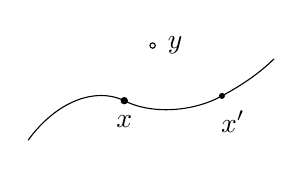
\begin{tikzpicture}[x=1cm,y=1cm,line cap=round]
\draw (0,0) .. controls (.35,.48) and (.84,.68) .. (1.22,.50)
.. controls (1.57,.32) and (2.10,.36) .. (2.46,.56)
.. controls (2.72,.70) and (2.95,.86) .. (3.12,1.03);
\fill (1.22,.50) circle (.047);
\fill (2.46,.56) circle (.038);
\draw (1.58,1.20) circle (.034);
\node[below] at (1.22,.43) {$x$};
\node[below] at (2.60,.49) {$x'$};
\node[right] at (1.65,1.20) {$y$};
\end{tikzpicture}}\endgroup
}
\end{GelfandAdjacentEvidence}
\begin{GelfandAdjacentEvidence}{GELFAND-P000988}{3}


$(x,y)\mapsto(x,x')$ невозможно, т.к. $\{x\}^{\mathrm{cl}}$ сох\textsuperscript{?}
\Unclear{GELFAND-P000988}{impossible-tail}{сох}
\end{GelfandAdjacentEvidence}
\begin{GelfandAdjacentEvidence}{GELFAND-P000988}{4}


На $\overline{\mathcal F}_I$ уже может действовать дважды транзитивно

\underline{Пример}

дважды транзит. на $F\Longleftrightarrow$ транзит. на $(F\times F)\setminus\Delta$
\[
\forall x\in F,\quad G_x\text{ должно транзит. действ. на }F\setminus\{x\}
\]
\SourceFigure{GELFAND-P000988}{diagonal-sketch}{Четырёхугольник с восходящей диагональю; в левом верхнем углу небольшой разрыв.\par\smallskip
\begingroup\color{black}\GelfandFitDiagram{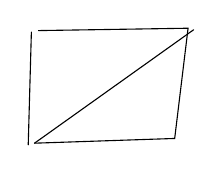
\begin{tikzpicture}[x=1cm,y=1cm,line cap=round]
\draw (0,0)--(.04,1.43);
\draw (.13,1.45)--(2.03,1.48)--(1.86,.08)--(.08,.02);
\draw (.08,.02)--(2.10,1.46);
\end{tikzpicture}}\endgroup
}
\end{GelfandAdjacentEvidence}
\begin{GelfandAdjacentEvidence}{GELFAND-P000988}{5}


Конец будет такой: для

$B,N,T,W,P$

даётся аксиоматич. обобщение, при к-ром имеет смысл разлож. Брюа.

\underline{При нек-рых усл. на действие:}

(i)
\[
\mathcal F_{\max}=\{\max\ \text{вполне упоряд. цепь}\quad
S_1<S_2<\cdots<S_i<\cdots
\]
[В конце строки зачёркнуто: запись не разобрана.]
\Unclear{GELFAND-P000988}{axiom1-cancel-end}{запись не разобрана}
\end{GelfandAdjacentEvidence}
\begin{GelfandAdjacentEvidence}{GELFAND-P000988}{6}


$S_i\in$ [зачёркнуто: запись не разобрана] $\mathcal F\}$
\Unclear{GELFAND-P000988}{axiom1-cancel-family}{запись не разобрана}
\end{GelfandAdjacentEvidence}
\begin{GelfandAdjacentEvidence}{GELFAND-P000988}{7}


[Под $\mathcal F_{\max}$:] (Флаги)

\SourceFigure{GELFAND-P000988}{flags-max-symbol}{У $\mathcal F_{\max}$ отдельная верхняя черта не видна.}
\end{GelfandAdjacentEvidence}
\begin{GelfandAdjacentEvidence}{GELFAND-P000988}{8}


\underline{транзит. относит. $G$}

(ii)
\[
\forall S:\ \dim(S)=\text{длина $\max$ флага},\quad<+\infty
\]
[Под $S$ приписано $\mathcal F$ со стрелкой вверх.]\SourceFigure{GELFAND-P000988}{dimension-pointer}{Стрелка от $\mathcal F$ указывает вверх к $S$.}
\end{GelfandAdjacentEvidence}
\begin{GelfandAdjacentEvidence}{GELFAND-P000988}{9}


[Под $\dim(S)$ зачёркнуто: запись не разобрана.]
\Unclear{GELFAND-P000988}{axiom2-cancel-under-dim}{запись не разобрана}
\end{GelfandAdjacentEvidence}
\begin{GelfandAdjacentEvidence}{GELFAND-P000988}{10}


[Под «длина $\max$ флага»: зачёркнуто запись не разобрана, затем:] заканчив. $S$.
\Unclear{GELFAND-P000988}{axiom2-cancel-before-ending}{запись не разобрана}
\end{GelfandAdjacentEvidence}
\begin{GelfandAdjacentEvidence}{GELFAND-P000988}{11}


(iii)
\[
S,S'\subseteq T,\quad\dim S+\dim S'>\dim(T)
\Rightarrow S\cap S'\ne\bigcap_{\mathcal F\ni T'}T'
\]
(iv) $\forall S\in\mathcal F$, если $\{x\}^{\mathrm{cl}}\cap S=$ $(\varnothing)^{\mathrm{cl}}$\textsuperscript{?}, то
\[
G^S\cap G^{\{x\}^{\mathrm{cl}}}
\underset{\text{отобр. \underline{\underline{на}}}}{\longrightarrow}
\overline{G^S}
\]
\Unclear{GELFAND-P000988}{axiom4-zero}{$(\varnothing)^{\mathrm{cl}}$}
\end{GelfandAdjacentEvidence}
\begin{GelfandAdjacentEvidence}{GELFAND-P000988}{12}

Тогда
\[
G=\coprod_WG^f wG^f\qquad\text{(несвязное объед.)}
\]
(двойной смежн. класс)

где
\[
G^f=\bigcap_I G^{f(i)},\qquad f:I\to\mathcal F
\]
[От $G^f$ выносная черта к подписи:] стабилизатор $\max$ флага.
\[
W=N/T
\]
[Над $f$ приписано «здесь».]
\[
\{f:I\to\mathcal F;\quad S_1<S_2<S_3<S_4<\cdots
\]
--- любая $\max$ цепь $\}$ \SourceFigure{GELFAND-P000988}{bottom-left-arrow}{Перед «любая» короткий штрих; отдельный наконечник не различим.}
\end{GelfandAdjacentEvidence}



\Needspace{7\baselineskip}
\begin{GelfandAdjacentEvidence}{GELFAND-P000989}{1}
\SourcePage{GELFAND-P000989}{unlabelled}
\underline{Задачи.} (И.М.Г.)

Описать 2-стор. классы смежности
\[
\begin{aligned}
1)&\quad U(n)\backslash GL(n)/U(n)\\
2)&\quad \underset{\substack{\diagup\\\text{треуг.}}}{B(n)}
             \backslash GL(n)/B(n)\\
3)&\quad U(n)\backslash GL(n)/B(n)
\end{aligned}
\]
\SourceFigure{GELFAND-P000989}{double-coset-leader}{Подпись «треуг.» соединена наклонной чертой с левым $B(n)$ в пункте 2.}
\end{GelfandAdjacentEvidence}
\begin{GelfandAdjacentEvidence}{GELFAND-P000989}{2}


$\forall\ \max$ флаг получ. так:
\[
f(i)=\operatorname{cl}(\{e_j\}_{j\leq i}),\quad
\text{где }\{e_j\}\text{ --- точки в }X.
\]
\[
C_i=\operatorname{cl}(\{e_i\})
\]
\[
N=\{g\mid g\text{ переставляет }\{C_i\}\}
\]
и мы имеем:

\SourceFigure{GELFAND-P000989}{middle-group-sequence}{Начальный знак обведён поверх прежних штрихов. Предположительно $1$ поверх $0$.\par\smallskip
\begingroup\color{black}\GelfandFitDiagram{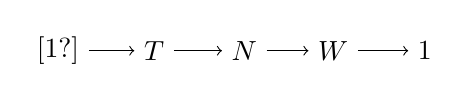
\begin{tikzpicture}[baseline=(a.base), x=.91cm]
\node (a) at (0,0) {$[1?]$};
\node (t) at (1.34,0) {$T$};
\node (n) at (2.60,0) {$N$};
\node (w) at (3.84,0) {$W$};
\node (one) at (5.12,0) {$1$};
\draw[->] (a)--(t);
\draw[->] (t)--(n);
\draw[->] (n)--(w);
\draw[->] (w)--(one);
\end{tikzpicture}}\endgroup
}
\end{GelfandAdjacentEvidence}
\begin{GelfandAdjacentEvidence}{GELFAND-P000989}{3}


$T$ сост. из тех, к-рые оставл. на месте каждое $C_i$;

$W=N/T$ по опред.

Докладчик не знает примеров, отл. от классических, где вып. все аксиомы.

Но: есть примеры, где разлож. [зачёркнуто: не (?)] есть, хотя аксиомы не выполн.
\Unclear{GELFAND-P000989}{lower-cancelled-word}{не (?)}
\end{GelfandAdjacentEvidence}
\begin{GelfandAdjacentEvidence}{GELFAND-P000989}{4}


\underline{Зелевинский.}

О работе \underline{S. Abeasis, A. Del Fra, H. Kraft.}

\underline{The geometry of repres. of $A_m$}, Math. Ann., 256, N.3,
401--418, (1981).

\SourceFigure{GELFAND-P000989}{lower-bibliography-pages}{Начальная страница читается $401$.}
\end{GelfandAdjacentEvidence}
\begin{GelfandAdjacentEvidence}{GELFAND-P000989}{5}


$A_m$ --- колчан

\SourceFigure{GELFAND-P000989}{lower-quiver}{У последней стрелки виден правый наконечник; у левого конца дополнительные штрихи. Над стрелкой написано $A_m$.\par\smallskip
\begingroup\color{black}\GelfandFitDiagram{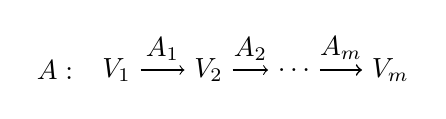
\begin{tikzpicture}[baseline=(a.base), x=.92cm]
\node (a) at (0,0) {$A:$};
\node (first) at (.85,0) {$V_1$};
\node (second) at (2.12,0) {$V_2$};
\node (dots) at (3.30,0) {$\ldots$};
\node (last) at (4.63,0) {$V_m$};
\draw[->] (first)--node[above] {$A_1$} (second);
\draw[->] (second)--node[above] {$A_2$} (dots);
\draw[->,semithick] (dots)--node[above] {$A_m$} (last);
\end{tikzpicture}}\endgroup
}
\end{GelfandAdjacentEvidence}
\begin{GelfandAdjacentEvidence}{GELFAND-P000989}{6}


--- это представл. колчана серии $A_m$.

Здесь действ. группа
\[
GL(V_1)\times\cdots\times GL(V_m).
\]
\SourceFigure{GELFAND-P000989}{bottom-group-index}{Первый индекс читается $1$.}
\end{GelfandAdjacentEvidence}
\begin{GelfandAdjacentEvidence}{GELFAND-P000989}{7}


Орбиты --- предст. с точн. до эквив.

Орбит конечное число. Они допус.\textsuperscript{?} явное опис.
\Unclear{GELFAND-P000989}{bottom-description-abbrev}{допус.}
\end{GelfandAdjacentEvidence}
\begin{GelfandAdjacentEvidence}{GELFAND-P000989}{8}


Их замык. --- хорошие мн-ия (нормальные, Коэн --- Маколея\textsuperscript{?} и т.п.).
\Unclear{GELFAND-P000989}{bottom-cohen-macaulay}{Маколея}
\end{GelfandAdjacentEvidence}



\Needspace{7\baselineskip}
\begin{GelfandAdjacentEvidence}{GELFAND-P000990}{1}
\SourcePage{GELFAND-P000990}{16}
[Зачёркнуто: Их (?)] Они аналогичны клеткам Шуберта и многочлены описывают предст. $p$-адич. групп, как геом. клеток Шуберта связана с предст. классич. групп.
\Unclear{GELFAND-P000990}{top-cancelled-word}{Их (?)}
\end{GelfandAdjacentEvidence}
\begin{GelfandAdjacentEvidence}{GELFAND-P000990}{2}


Для

\SourceFigure{GELFAND-P000990}{first-linear-arrow}{Стрелка от $V_1$ к $V_2$ с меткой $A_1$.\par\smallskip
\begingroup\color{black}\GelfandFitDiagram{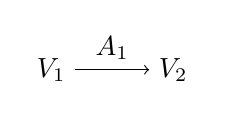
\begin{tikzpicture}[baseline=(first.base)]
\node (first) at (0,0) {$V_1$};
\node (second) at (1.55,0) {$V_2$};
\draw[->] (first)--node[above] {$A_1$} (second);
\end{tikzpicture}}\endgroup
}
\end{GelfandAdjacentEvidence}
\begin{GelfandAdjacentEvidence}{GELFAND-P000990}{3}

возникают детерминантные мн-ия.

Описание орбит:

\SourceFigure{GELFAND-P000990}{upper-composition-arrow}{Под $V_i$ отдельный знак со штрихами; точное чтение не установлено.\par\smallskip
\begingroup\color{black}\GelfandFitDiagram{\begin{tikzpicture}[baseline=(first.base)]
\node (first) at (0,0) {$V_i$};
\node (second) at (2.45,0) {$V_j$};
\draw[->] (first)--node[below] {композ.} (second);
\node[below=3pt] at (first.south) {$[?]$};
\end{tikzpicture}}\endgroup
}
\end{GelfandAdjacentEvidence}
\begin{GelfandAdjacentEvidence}{GELFAND-P000990}{4}


Надо задать \underline{ранги всевозм. композиций} $r_{ij}$.

Должна быть вып. система нер-в.

Есть другое опис. через кратности вхождений.

\underline{\underline{19/X-81 г.}}\qquad\underline{Сем. Гельфанда.}

\underline{Кириллов.}

Как устр. алгебра Ли с образующими $x,y$ и соотн.
\[
(\operatorname{ad}x)^{a+1}y=0,\qquad
(\operatorname{ad}y)^{b+1}x=0,\qquad a,b\in\mathbb{N}.
\]
\SourceFigure{GELFAND-P000990}{dimension-table}{Ось $a$ вправо, $b$ вниз. В ячейках $(a,b)=(3,2),(2,3)$ стоят вопросительные знаки. Остальные пустые ячейки оставлены пустыми.\par\smallskip
\begingroup\color{black}\GelfandFitDiagram{\begin{tikzpicture}[x=.55cm,y=.48cm,font=\small]
\draw[->] (.1,0)--(5.8,0) node[right] {$a$};
\draw[->] (0,-.09)--(0,-6.4) node[below left] {$b$};
\foreach \i in {1,2,3,4} {
 \node at (\i-.46,.43) {$\i$};
 \node at (-.43,-\i+.47) {$\i$};
}
\node at (.54,-.53) {$3$};
\node at (1.54,-.53) {$4$};
\node at (2.54,-.53) {$6$};
\node at (3.54,-.53) {$\infty$};
\node at (.54,-1.53) {$4$};
\node at (1.54,-1.53) {$\infty$};
\node at (2.54,-1.53) {$?$};
\node at (.54,-2.53) {$6$};
\node at (1.54,-2.53) {$?$};
\node at (.54,-3.53) {$\infty$};
\draw[<-] (3.83,-1.60)--(4.53,-1.60);
\node[anchor=north west,align=left,font=\scriptsize] at (4.28,-2.00) {размерности в тех\\случаях, когда они\\известны.};
\end{tikzpicture}}\endgroup
}
\end{GelfandAdjacentEvidence}
\begin{GelfandAdjacentEvidence}{GELFAND-P000990}{5}


\underline{Без соотношений} число коммов бистепени $k,\ell$ равно:
\[
d(k,\ell)=\frac{1}{k+\ell}\sum_{d\mid(k,\ell)}
\mu(d)\,\frac{\left(\frac{k}{d}+\frac{\ell}{d}\right)!}
{\frac{k}{d}!\,\frac{\ell}{d}!}.
\]
$k=n$, $\ell=n+1$ $\Rightarrow$ $n$-е число Каталана

($=$ число способов расстан. скобок в неассоциат. произведении $x\cdot x\cdot\ldots\cdot x$.)

[Слева выше следующей строки: $(\sim)$.]

Другой вопрос: оберт. алгебра.

\underline{Соотн.}
\begin{align*}
0&=x^{a+1}y-\binom{a+1}{1}x^ayx+\binom{a+1}{2}x^{a-1}yx^2+\ldots\,,\\
0&=y^{b+1}x-\binom{b+1}{1}y^bxy+\binom{b+1}{2}y^{b-1}xy^2-\ldots\,.
\end{align*}
\SourceFigure{GELFAND-P000990}{lower-relation-signs}{Перед многоточием в первой строке стоит $+$, во второй $-$.}
\end{GelfandAdjacentEvidence}
\begin{GelfandAdjacentEvidence}{GELFAND-P000990}{6}


$V$ --- вект. пр-во, \qquad $S(\bar V)=e^{\bar V}$ --- симм. алгебра

[Под «$V$ --- вект. пр-во»: «(градуир.)».]

$p(t)=\sum t^k\dim V_k$ --- многочлен Гильберта.
\Unclear{GELFAND-P000990}{bottom-hilbert-letter}{$p(t)$}
\end{GelfandAdjacentEvidence}



\Needspace{7\baselineskip}
\begin{GelfandAdjacentEvidence}{GELFAND-P000991}{1}
\SourcePage{GELFAND-P000991}{unlabelled}
$k$ --- вес $\Rightarrow$ возникает вес на $S(V)$
$\Rightarrow$ градуир. на $S(V)$
$\Rightarrow$ полином Гильберта вычисляется $P(t)$ для $S(V)$
(или форм. ряд).

Связь:

[Зачёркнуто: формула не разобрана.]
\Unclear{GELFAND-P000991}{series-cancelled-01}{формула не разобрана}
\end{GelfandAdjacentEvidence}
\begin{GelfandAdjacentEvidence}{GELFAND-P000991}{2}

\[
\ln P(t)=\sum\frac{C_k}{k}t^k;
\]
[Зачёркнуто: короткая запись не разобрана.]
\Unclear{GELFAND-P000991}{series-cancelled-02}{короткая запись не разобрана}
\end{GelfandAdjacentEvidence}
\begin{GelfandAdjacentEvidence}{GELFAND-P000991}{3}

\[
p(t)=\sum\frac{c_k}{k}t^k,\qquad C_k=\sum_{d\mid k}c_d.
\]
\SourceFigure{GELFAND-P000991}{series-coefficient}{В выражении для $p(t)$ в знаменателе стоит $k$, а в числителе $c_k$.}
\end{GelfandAdjacentEvidence}
\begin{GelfandAdjacentEvidence}{GELFAND-P000991}{4}

\[
\underline{x^{k_1}y^{\ell_1}x^{k_2}y^{\ell_2}\ldots x^{k_n}y^{\ell_n}}
\]
\[
\begin{aligned}
k_1+k_2+\ldots+k_n&=k,\\
\ell_1+\ell_2+\ldots+\ell_n&=\ell.
\end{aligned}
\]
Лексикограф. упоряд.

\underline{$y$ старше $x$}. \qquad $x<y$.

\underline{И.М.Г.} \quad \underline{комбин. задача}

$m_1\le m_2\le m_3\le m_4$ --- \underline{фиксир.}

\SourceFigure{GELFAND-P000991}{table-interlacing}{Четыре ряда кружков: $4,3,2,1$. Стрелка от пояснения слева указывает на первый кружок второго ряда.\par\smallskip
\begingroup\color{black}\GelfandFitDiagram{\begin{tikzpicture}[x=.87cm,y=.82cm,
  dot/.style={circle,draw,inner sep=1.65pt,outer sep=1.35pt}]
\node[dot] (a1) at (0,0) {};
\node[dot] (a2) at (1,0) {};
\node[dot] (a3) at (2,0) {};
\node[dot] (a4) at (3,0) {};
\node[dot] (b1) at (.50,-.74) {};
\node[dot] (b2) at (1.50,-.74) {};
\node[dot] (b3) at (2.50,-.74) {};
\node[dot] (c1) at (1,-1.46) {};
\node[dot] (c2) at (2,-1.46) {};
\node[dot] (d1) at (1.50,-2.23) {};
\draw (a1)--(b1)--(a2)--(b2)--(a3)--(b3)--(a4);
\draw (b1)--(c1)--(b2)--(c2)--(b3);
\draw (c1)--(d1)--(c2);
\node[align=left,anchor=north east,font=\scriptsize] (note) at (-.48,-1.48)
  {между\\$m_1$ и $m_2$\\(вкл. концы)};
\draw[->] (note.north east)--(b1.south west);
\end{tikzpicture}}\endgroup
}
\end{GelfandAdjacentEvidence}


\underline{ск. таблиц?}

($=$ сколько предст. $SL(4)$ с зад. старшим весом?)

см. добавл. к книге Гельфанд--Минлос--Шапиро.


\Needspace{7\baselineskip}
\begin{GelfandAdjacentEvidence}{GELFAND-P000992}{1}
\SourcePage{GELFAND-P000992}{unlabelled}
\underline{\underline{16.11.81 г.}} \qquad \underline{Сем. Гельфанда.}

\underline{\underline{А.С. Шварц.}} \qquad \underline{Геометрия супергравитации.}

$\mathbb R^{p,q}$ --- суперпр-во\qquad
$(x^1,\ldots,x^p,\theta^1,\ldots,\theta^q)$.

$\Lambda$ --- грассм. алг.
[Над сокращением: г или 4\textsuperscript{?}.]
\Unclear{GELFAND-P000992}{algebra-insertion}{г или 4}
\end{GelfandAdjacentEvidence}
\begin{GelfandAdjacentEvidence}{GELFAND-P000992}{2}

[Зачёркнуто: запись не разобрана.]
\Unclear{GELFAND-P000992}{algebra-cancelled-01}{запись не разобрана}
\end{GelfandAdjacentEvidence}
\begin{GelfandAdjacentEvidence}{GELFAND-P000992}{3}

[Зачёркнуто: с градуировкой\textsuperscript{?}.]
\Unclear{GELFAND-P000992}{algebra-cancelled-02}{с градуировкой}
\end{GelfandAdjacentEvidence}
\begin{GelfandAdjacentEvidence}{GELFAND-P000992}{4}

(над $\mathbb R$).

$\mathbb R^{p,q}_{\Lambda}$ --- пр-во строчек
$(x^1,\ldots,x^p,\theta^1,\ldots,\theta^q)$,
где $x^j$ --- чётные элем. $\Lambda$, $\theta^j$ --- нечётные элем. $\Lambda$.

Нужно рассм. это как функтор от $\Lambda$ (неудобно\textsuperscript{?} фиксировать $\Lambda$).
\Unclear{GELFAND-P000992}{functor-parenthesis}{неудобно}
\end{GelfandAdjacentEvidence}
\begin{GelfandAdjacentEvidence}{GELFAND-P000992}{5}


Получается $\mathbb R^{p,q}$.

$\mathbb C^{p,q}$ опред. аналогично и в нём опред. инволюция.

\medskip
Рассм. $\mathbb C^{4,2}$ \qquad $(x^m,\theta^\alpha)=z^A$.
\[
\dim_{\mathbb C}\mathbb C^{4,2}=(4,2),\qquad
\dim_{\mathbb R}(\mathbb C^{4,2})=(8,4).
\]
В нём рассм. веществ. подмн-зие
\[
\begin{array}{cl}
\Omega & \subset\mathbb C^{4,2}\\[-1pt]
(4,4)&\leftarrow\underline{\mathbb R}\text{-dim}
\end{array}
\]
\SourceFigure{GELFAND-P000992}{omega-dimension}{Под $\Omega$ написано $(4,4)$, к нему ведёт стрелка от подписи $\underline{\mathbb R}$-dim.}
\end{GelfandAdjacentEvidence}


$\Omega$ выд. ур-ями
\[
f^k(z,\bar z)=0,
\]
$f^k$ --- чётные вещественные, \quad $k=1,2,3,4$.

Рассм. в $\mathbb C^{4,2}$ аналит. преобр-я:
\[
\begin{cases}
\widetilde{x}^{a}=\lambda^{a}(x,\theta),\\
\widetilde{\theta}^{\alpha}=\lambda^{\alpha}(x,\theta)
\end{cases}
\qquad
\text{(не завис. от $\bar x,\bar\theta$)}.
\]


\Needspace{7\baselineskip}
\begin{GelfandAdjacentEvidence}{GELFAND-P000993}{1}
\SourcePage{GELFAND-P000993}{40}
Они образуют супергруппу $L$.

(Группа зависит от $\Lambda$ и всё вместе --- функтор из грассм. алг. в обычные группы --- супергруппы.)

Рассм. те, к-рые сохраняют \underline{суперобъём}.
\[
\widetilde z^{A}=\lambda^{A}(z).
\]
Сохр. объёма:
\[
\operatorname{Ber}\frac{\partial\widetilde z^{A}}{\partial z^{B}}=1.
\]
Будем рассм. ф-ал
\[
S(\Omega)=\int A\bigl(\text{перв., втор. произв. }f^k\bigr)
\prod_k\delta\bigl(f^k(z,\bar z)\bigr)\,dz\,d\bar z.
\]
[В аргументе $A$, перед $f^k$, зачёркнуто: $f^k$\textsuperscript{?}.]
\Unclear{GELFAND-P000993}{functional-cancelled}{$f^k$}
\end{GelfandAdjacentEvidence}
\begin{GelfandAdjacentEvidence}{GELFAND-P000993}{2}


[К $\delta$ проведена черта с подписью: $\delta$-ф-я.]\SourceFigure{GELFAND-P000993}{delta-label}{Под $\delta$ стоит пояснение «$\delta$-ф-я».}
\end{GelfandAdjacentEvidence}
\begin{GelfandAdjacentEvidence}{GELFAND-P000993}{3}


На $A$ налож. такое усл., чтобы $S(\Omega)$ зависел лишь от $\Omega$, а не от её ур-й.

В классич. теор. поля, вместо поля $\varphi$ можно рассм. график ф-и --- поверхность.

\SourceFigure{GELFAND-P000993}{field-graph}{График с минимумом выше горизонтальной оси $x$, вертикальная ось $\varphi$.\par\smallskip
\begingroup\color{black}\GelfandFitDiagram{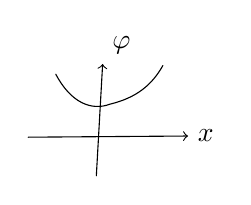
\begin{tikzpicture}[x=1cm,y=1cm,line cap=round]
\draw[->] (-.90,0)--(1.13,.015) node[right] {$x$};
\draw[->] (-.035,-.49)--(.045,.93) node[above right] {$\varphi$};
\draw (-.55,.80) .. controls (-.36,.44) and (-.10,.33) .. (.14,.42)
 .. controls (.47,.50) and (.67,.66) .. (.81,.91);
\end{tikzpicture}}\endgroup
}
\end{GelfandAdjacentEvidence}
\begin{GelfandAdjacentEvidence}{GELFAND-P000993}{4}


Рассм. $\Omega$ как график поля
\[
\mathbb R^{4,4}\longrightarrow\mathbb R^{4,0},\qquad
H^m(\xi,\theta,\bar\theta).
\]
\Unclear{GELFAND-P000993}{superfield-argument}{Первый аргумент сильно обведён; предположительно $\xi$.}
\end{GelfandAdjacentEvidence}
\begin{GelfandAdjacentEvidence}{GELFAND-P000993}{5}


Пов. $\Omega$ и суперполе находятся во вз.-однозн. соотв.

\underline{Действие супергравитации:} \underline{единств.} (с точн. до множ.) ф-л \underline{такого вида, инвариантный отн. группы $L$}.

Тогда $S(\Omega)$ варьируя получим\textsuperscript{?}.
\Unclear{GELFAND-P000993}{variation-last-word}{получим}
\end{GelfandAdjacentEvidence}
\begin{GelfandAdjacentEvidence}{GELFAND-P000993}{6}


А именно:
\[
A=|\det\Gamma|^{-1/2},\qquad
\Gamma\text{ --- форма Леви поверхности }\Omega.
\]
\SourceFigure{GELFAND-P000993}{levi-power}{Перед дробью $1/2$ виден минус.}
\end{GelfandAdjacentEvidence}
\begin{GelfandAdjacentEvidence}{GELFAND-P000993}{7}


[Под «форма» вписано «(супер.)».]

Форма Леви --- 1-я \underline{структ. ф-а} $CR$-структуры.

Форма
\[
\left.
\frac{\partial^2 f^k}{\partial z^A\partial\bar z^B}\,
dz^A\,d\bar z^B
\ \right|_{\substack{\text{на компл. кас. плоскости}\\
 \frac{\partial f^k}{\partial z^A}dz^A=0}}
\]
(вект-нозначная)

[Зачёркнуто: $\partial f$.]\SourceFigure{GELFAND-P000993}{levi-cancellation}{Над «наз. формой Леви» зачёркнуто $\partial f$.}
\end{GelfandAdjacentEvidence}
\begin{GelfandAdjacentEvidence}{GELFAND-P000993}{8}


\underline{наз. формой Леви $\Gamma$}.

\SourceFigure{GELFAND-P000993}{levi-pointer}{От слов о касательной плоскости стрелка вниз к пояснению о размерности.}
\end{GelfandAdjacentEvidence}


она имеет размерность $(0,2)$.
\[
\frac{\partial f^k}{\partial x^a}\,dx^a+
\frac{\partial f^k}{\partial\theta^\alpha}\,d\theta^\alpha=0
\]
\[
\Rightarrow dx^a\text{ выраж. через }d\theta^\alpha
\Rightarrow \text{разм. }(0,2).
\]


\Needspace{7\baselineskip}
\begin{GelfandAdjacentEvidence}{GELFAND-P000994}{1}
\SourcePage{GELFAND-P000994}{unlabelled}
Базис в компл. кас. плоск. выб. по-разному.

Det. (?) от этого зависит.
\Unclear{GELFAND-P000994}{det-overwritten}{Начальные штрихи сокращения «Det.» переписаны.}
\end{GelfandAdjacentEvidence}
\begin{GelfandAdjacentEvidence}{GELFAND-P000994}{2}

\[
\Gamma^k_{\alpha\dot\beta}
\qquad
\begin{aligned}
k&\text{ --- 4 возможности},\\
\alpha,\dot\beta&\text{ --- 4 возможности}\quad(2\times2=4).
\end{aligned}
\]
\SourceFigure{GELFAND-P000994}{levi-indices}{В нижнем индексе $\Gamma$ точка стоит над $\beta$.}
\end{GelfandAdjacentEvidence}
\begin{GelfandAdjacentEvidence}{GELFAND-P000994}{3}

\underline{\underline{$\det$}} --- $\det$ \underline{такой $4\times4$-матрицы}.

Она и $\det$ зависит от выб. базиса.

Надо [зачёркнуто: неразборчиво] прав. выб. базис в компл. кас. плоскости.
\Unclear{GELFAND-P000994}{basis-cancelled}{Сочетание после «Надо» зачёркнуто, чтение не установлено.}
\end{GelfandAdjacentEvidence}
\begin{GelfandAdjacentEvidence}{GELFAND-P000994}{4}


Для функций: естеств. выб. базиса
\[
\Gamma^k_{\alpha\dot\beta}\,d\theta^\alpha\,d\overline{\theta^\beta}.
\]
\Unclear{GELFAND-P000994}{levi-differential-index}{У второго дифференциала неясны предел надчёркивания и точка у верхнего индекса: $d\overline{\theta^\beta}$ или $d\bar\theta^{\dot\beta}$.}
\end{GelfandAdjacentEvidence}
\begin{GelfandAdjacentEvidence}{GELFAND-P000994}{5}


и тогда надо писать
\[
A=\left(\det\frac{\partial f^k}{\partial z^a}\right)^{4/3}
|\det\Gamma|^{-1/3}.
\]
\Unclear{GELFAND-P000994}{density-denominator}{В знаменателе предположительно $z^a$, возможно $x^a$. Буква переписана.}
\end{GelfandAdjacentEvidence}
\begin{GelfandAdjacentEvidence}{GELFAND-P000994}{6}


см. \underline{Ядерная физика}, 1981, $N=10$.

предв. больш. (?) раб. \underline{Nuclear Physics}, 1981.

[Обе ссылки объединены правой скобкой с подписью:] \underline{А.С. Шварц}.

[Справа:] ещё есть что-то в \underline{Communic. Math. Phys.}
\SourceFigure{GELFAND-P000994}{bibliography-brace}{Справа от скобки стоят имя и отдельная помета о журнале.}
\end{GelfandAdjacentEvidence}
\begin{GelfandAdjacentEvidence}{GELFAND-P000994}{7}

\Unclear{GELFAND-P000994}{bibliography-abbreviations}{Перед «Nuclear Physics» предположительно «предв. больш. раб.».}
\end{GelfandAdjacentEvidence}
\begin{GelfandAdjacentEvidence}{GELFAND-P000994}{8}


$G$-структ. на компл. мн-зии (?) $\Rightarrow CR$-структура на поверхности.
\Unclear{GELFAND-P000994}{manifold-abbreviation}{После «на компл.» сокращение с дефисом, предположительно «мн-зии».}
\end{GelfandAdjacentEvidence}


($\sim$ компл. стр. $GL(n,\mathbb C)$)

Здесь $SL(4,2\mid\mathbb C)$ --- структура.

$L$ --- группа автом. этой структ.

На пов. возникает $SCR$-структура, отлич. от $CR$ $\det$ условием.

В $\mathbb C^{4,2}$ перепутаны координаты и значения полей и их нельзя рассм. отдельно.

\begin{center}$-\ \cdot\ -$\end{center}


\Needspace{7\baselineskip}
\begin{GelfandAdjacentEvidence}{GELFAND-P000995}{1}
\SourcePage{GELFAND-P000995}{unlabelled}
\underline{23.11.81 г.}\qquad\underline{\underline{Сем. Гельфанда.}}

\underline{Зелевинский}.

$\mathfrak g$ --- компл. полупр. алг. Ли.
\[
\mathfrak g\supset
\underset{\text{борел.}}{\mathfrak b}\supset
\underset{\text{карт.}}{\mathfrak h}.
\]
\underline{Пример.}\quad $\mathfrak{sl}_n$\qquad [под $\mathfrak b$: «верхн. треугл.», под $\mathfrak h$: «диаг.»].
\[
\underbrace{
 \overbrace{e_1,\ldots,e_n}^{\mathfrak n_+},
 \overbrace{h_1,\ldots,h_n}^{\mathfrak h}
}_{\mathfrak b_+},
\quad f_1,\ldots,f_n.
\]
\SourceFigure{GELFAND-P000995}{generator-brackets}{Две верхние скобки отмечены $\mathfrak n_+$ и $\mathfrak h$, общая нижняя --- $\mathfrak b_+$.}
\end{GelfandAdjacentEvidence}
\begin{GelfandAdjacentEvidence}{GELFAND-P000995}{2}


\underline{Предст.:} $e_j\mapsto E_j$ и т.д.

Старший вес! вектор $x$: $E_jx=0$, $j=1,\ldots,n$.
\SourceFigure{GELFAND-P000995}{highest-weight-exclamation}{После «вес» стоит знак, читаемый как «!».}
\end{GelfandAdjacentEvidence}
\begin{GelfandAdjacentEvidence}{GELFAND-P000995}{3}


$\Rightarrow H_jx$ --- тоже старший вес.

Всегда $\exists$ в конечномерном предст.

\underline{Модуль Верма}

$\chi\in\mathfrak h^*$.

[Зачёркнуто: «Старш.» (?)] Вектор старш. веса $\chi$:
\[
\begin{cases}
ev=0,&\forall e\in\mathfrak n_+,\\
hv=\chi(h)v,&\forall h\in\mathfrak h.
\end{cases}
\]
\Unclear{GELFAND-P000995}{highest-weight-cancelled}{Зачёркнутая запись предположительно «Старш.».}
\end{GelfandAdjacentEvidence}
\begin{GelfandAdjacentEvidence}{GELFAND-P000995}{4}


\underline{Модуль Верма:} наибольший модуль $M(\chi)$, порожд. старш. весом $\chi$.

(Универс. модуль с этими св-вами.)

$M(\chi)$ не явл. непривод. (вообще говоря).

$L(\chi)$ --- единств. непривод. фактормодуль $M(\chi)$.

\underline{Теор.} $\exists$ конечн. композиц. ряд
\[
M(\chi)=M_1\supset M_2\supset\ldots\supset M_n=0,
\qquad M_i/M_{i+1}=L(\chi_i).
\]
$\Rightarrow$ любой подфактор имеет такой вид.

\underline{Вопрос:} дано $\psi$, какова кратность вхожд. $M(\psi)$ в композиц. ряд мод. Верма.
\SourceFigure{GELFAND-P000995}{multiplicity-module-letter}{В вопросе написано $M(\psi)$.}
\end{GelfandAdjacentEvidence}
\begin{GelfandAdjacentEvidence}{GELFAND-P000995}{5}


(Это экв. опис. [вписано: «самого»] мод. Верма.)
[Под скобками: «--- можно посчитать».]
\SourceFigure{GELFAND-P000995}{itself-insertion}{Слово «самого» над строкой снабжено знаком вставки.}
\end{GelfandAdjacentEvidence}
\begin{GelfandAdjacentEvidence}{GELFAND-P000995}{6}


Обознач. кратности
\[
m(\chi,\psi)=[M(\chi):L(\psi)].
\]

Кратности $=$ значение нек-рого многочлена в т. 1.
\Unclear{GELFAND-P000995}{polynomial-abbreviation}{Сокращение перед «многочлена» читается «нек-рого».}
\end{GelfandAdjacentEvidence}
\begin{GelfandAdjacentEvidence}{GELFAND-P000995}{7}


\underline{Условие:}
\[
\chi+\rho\in W(\psi+\rho),\quad
\text{т.е.}\quad \chi+\rho=w(\psi+\rho).
\]
[К $W$ подпись: «гр. Вейля».]

$\rho$ опр. ф-лой $\rho(h_i)=1$.

Только тогда кратность $m(\chi,\psi)$ может быть $\ne0$.

$\chi$ \underline{целочисл. доминантный} если $\lambda(h_i)\in\{0,1,2,\ldots\}$ для всех $h_i$.
\SourceFigure{GELFAND-P000995}{dominance-variable}{В условии после «если» стоит $\lambda(h_i)$, хотя строка начинается с $\chi$.}
\end{GelfandAdjacentEvidence}



\Needspace{7\baselineskip}
\SourcePage{GELFAND-P000996}{46}
\underline{Наш случай:}

$\chi_0$ --- целоч. домин. и
\begin{gather*}
\chi+\rho=w_1(\chi_0+\rho)\\
\psi+\rho=w_2(\chi_0+\rho)
\end{gather*}
Тогда
\[
m(\chi,\psi)=m(w_1,w_2)
\]
(не зависит от выб. домин. веса $\chi_0$).


\begin{GelfandAdjacentEvidence}{GELFAND-P000996}{1}
\underline{Каждан--Люстиг} --- гипотетич. выраж.

Теперь док.: Бейлинсон, Бернштейн. Брылинский, Кашивара.

Они выписали:
\[
P_{w_1,w_2}(q)
\]
--- полином (с неотриц. коэффициентами).

\underline{Гипотеза}
\[
m(w_1,w_2)=P_{w_1,w_2}(1).
\]
\[
P_{w_1,w_2}(q)=\sum a_iq^i.
\]
Смысл $a_i$ --- ?

Объяснение: $\exists$ фильтрация Янцена
\[
M(\chi)\supset M_1\supset M_2\supset\cdots
\]
$a_i={}$ кратность $L(\psi)$ в $M_i/M_{i+1}$.

\underline{Бейлинсон.}

\underline{Фильтрация Янцена.}

Двойств. модуль \({}^*M(\chi)\).

Общее определение: через категорию $O$.

$O$ --- кат. конечно-пор. мод., [над строкой вписано: $\mathfrak h$-]диагонализ., [зачёркнуто: неразборчиво], где [зачёркнуто: неразборчиво] [над строкой вместо зачёркнутого: $\mathfrak n_-$ (?) действ. лок. нильпотентно].
\Unclear{GELFAND-P000996}{category-cancelled-01}{Штрихи после «диагонализ.» густо зачёркнуты.}
\end{GelfandAdjacentEvidence}
\begin{GelfandAdjacentEvidence}{GELFAND-P000996}{2}

\Unclear{GELFAND-P000996}{category-cancelled-02}{Запись после «где» зачёркнута, точное чтение не установлено.}
\end{GelfandAdjacentEvidence}
\begin{GelfandAdjacentEvidence}{GELFAND-P000996}{3}

\Unclear{GELFAND-P000996}{nilpotent-sign}{У знака после $\mathfrak n$ наложены штрихи. Чтение «$-$» предположительно.}
\end{GelfandAdjacentEvidence}
\begin{GelfandAdjacentEvidence}{GELFAND-P000996}{4}


На ней опр. естеств. инволюция $*:O\longrightarrow O$.

(Двойственное предст. --- \underline{сопр. пр-во}. Оно беск. порожд., но в нём есть \underline{подпредст.}, сост. из ф-й, к-рые под действ. $\mathfrak h$ преобр. конечномер.)
\SourceFigure{GELFAND-P000996}{dual-last-word}{Конец строки читается «преобр. конечномер.».}
\end{GelfandAdjacentEvidence}
\begin{GelfandAdjacentEvidence}{GELFAND-P000996}{5}


[Приписка со стрелкой к предыдущей строке:] Здесь только $\mathfrak n_+$, а не $\mathfrak n_-$, но это безразлично.
\SourceFigure{GELFAND-P000996}{margin-plus-minus}{В приписке после $\mathfrak n_+$ стоит «а не $\mathfrak n_-$».}
\end{GelfandAdjacentEvidence}
\begin{GelfandAdjacentEvidence}{GELFAND-P000996}{6}


\underline{С. Гельфанд.}

На каждом $M(\chi)$ введём билин. форму со знач. в числах.
\[
M(\chi)\ni f_{i_1}\ldots f_{i_k}v,\qquad
v\text{ --- вектор старш. веса}.
\]
\SourceFigure{GELFAND-P000996}{form-module-parentheses}{Вес в записи перед знаком $\ni$ заключён в скобки.}
\end{GelfandAdjacentEvidence}
\begin{GelfandAdjacentEvidence}{GELFAND-P000996}{7}

\[
(f_{i_1}\ldots f_{i_k}v,\ f_{j_1}\ldots f_{j_l}v)
=
\begin{cases}
0\quad\text{при }\{i\}\ne\{j\}
 & \text{--- (неупоряд. мн-ва)},\\
\bigl(e_{i_1\ldots i_k}f_{j_1\ldots j_l}v\bigr)/v
 & \text{(вект. в числит. кратен $v$)}.
\end{cases}
\]
\SourceFigure{GELFAND-P000996}{form-multiindices}{В числителе у каждого из одиночных $e$ и $f$ записана последовательность индексов.}
\end{GelfandAdjacentEvidence}



\Needspace{7\baselineskip}
\begin{GelfandAdjacentEvidence}{GELFAND-P000997}{1}
\SourcePage{GELFAND-P000997}{unlabelled}
Получаем инвар. отн. алг. Ли форму.

[Зачёркнуто: неразборчиво] Будем отождествлять все $M(\chi)$ (для разных $\chi$) след. образом
\[
f_{i_1}\ldots f_{i_l}v_\chi
\longrightarrow f_{i_1}\ldots f_{i_l}v_{\chi'}.
\]
\Unclear{GELFAND-P000997}{top-cancelled}{Короткая запись перед «Будем» зачёркнута.}
\end{GelfandAdjacentEvidence}
\begin{GelfandAdjacentEvidence}{GELFAND-P000997}{2}


Рассм. $M(\chi)$ с [зачёркнуто: неразборчиво] фиксир. $\chi$ и затем рассм. $M(\chi+t\rho)$.
\Unclear{GELFAND-P000997}{fixed-cancel}{Между «с» и «фиксир.» зачёркнута короткая запись.}
\end{GelfandAdjacentEvidence}
\begin{GelfandAdjacentEvidence}{GELFAND-P000997}{3}


Получим много билин. форм на одном пр-ве:
\[
(\ ,\ )_t.
\]
Счит. все их формами на $M(\chi)$.

При малых $t\ne0$ форма невырождена.

\underline{Опред.}
\[
M_i=\{x\in M_\chi\mid (x,y)_t=O(t^i)\}.
\]
[Над условием со знаком вставки:] $\forall y\in M(\chi):$
\SourceFigure{GELFAND-P000997}{filtration-quantifier}{К условию приписано $\forall y\in M(\chi)$ с двоеточием.}
\end{GelfandAdjacentEvidence}
\begin{GelfandAdjacentEvidence}{GELFAND-P000997}{4}


Это и есть фильтр. Янцена.

Она --- фильтр. $\mathfrak g$-подмодулями.

Что если сменить $\rho$? Видимо, кратн. не будут меняться.

Полином
\[
P_{w_1,w_2}(q)=\sum q^i\bigl([L_\psi:M_i/M_{i+1}]\bigr),
\]
\SourceFigure{GELFAND-P000997}{multiplicity-order}{В рукописи $L_\psi$ стоит перед двоеточием, а $M_i/M_{i+1}$ после него.}
\end{GelfandAdjacentEvidence}
\begin{GelfandAdjacentEvidence}{GELFAND-P000997}{5}


где
\begin{gather*}
\psi=w_2(\chi_0+\rho)-\rho,\\
M_i\subset M_\chi,\qquad\chi=w_1(\chi_0+\rho)-\rho.
\end{gather*}
$P_{w_1,w_2}$ --- рекурр. определяются.
\[
a_i=\dim H^i\bigl(\text{по Макферсону одной клетки Шуберта вблизи другой}\bigr).
\]
(лок. когомол. нормального сечения)
\SourceFigure{GELFAND-P000997}{normal-section-sketch}{Наклонная линия с выделенной точкой, дуга и короткий отрезок к этой точке. Подписей нет.\par\smallskip
\begingroup\color{black}\GelfandFitDiagram{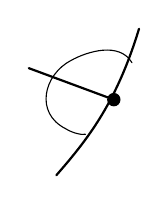
\begin{tikzpicture}[x=1cm,y=1cm,line cap=round]
\draw[thick] (.43,0) .. controls (.85,.48) and (1.20,.94) .. (1.48,1.86);
\draw (1.39,1.43) .. controls (1.23,1.70) and (.82,1.57) .. (.62,1.46)
 .. controls (.27,1.28) and (.15,.79) .. (.55,.59)
 .. controls (.63,.54) and (.74,.51) .. (.80,.52);
\draw[thick] (.08,1.36)--(1.16,.96);
\fill (1.16,.96) circle (.085);
\end{tikzpicture}}\endgroup
}
\end{GelfandAdjacentEvidence}
\begin{GelfandAdjacentEvidence}{GELFAND-P000997}{6}


или [зачёркнуто: неразборчиво] лок. относительные (?)

кл. $\subset$ др. клетка.
\Unclear{GELFAND-P000997}{geometric-cancelled}{После «или» слово зачёркнуто.}
\end{GelfandAdjacentEvidence}
\begin{GelfandAdjacentEvidence}{GELFAND-P000997}{7}

\Unclear{GELFAND-P000997}{geometric-note}{Запись читается предположительно «лок. относительные».}
\end{GelfandAdjacentEvidence}
\begin{GelfandAdjacentEvidence}{GELFAND-P000997}{8}


\underline{Зелевинский.}\quad\underline{Другие зад., те же многочл.}
\SourceFigure{GELFAND-P000997}{zelevinsky-heading}{В заголовке после «те же» сокращение «многочл.».}
\end{GelfandAdjacentEvidence}
\begin{GelfandAdjacentEvidence}{GELFAND-P000997}{9}


Рассм. конечномерное неприв. предст.
\[
L(\chi)=\bigoplus_\lambda L(\chi)_\lambda.
\]
[Под $L(\chi)_\lambda$, соединено чертой:] вес. пр-во с весом $\chi$.
\SourceFigure{GELFAND-P000997}{weight-annotation}{Подпись оканчивается буквой $\chi$.}
\end{GelfandAdjacentEvidence}
\begin{GelfandAdjacentEvidence}{GELFAND-P000997}{10}


\underline{И. М. Г.} Хорошая ф-я для $\dim L(\chi)_\lambda$ известна
\[
\begin{vmatrix}
x_1^{a_1}&x_2^{a_1}&\ldots&x_n^{a_1}\\
x_1^{a_2}&x_2^{a_2}&\ldots&x_n^{a_2}\\
x_1^{a_n}&x_2^{a_n}&\ldots&x_n^{a_n}
\end{vmatrix}
:
\begin{vmatrix}
1&\ldots&1\\
x_1&\ldots&x_n\\
x_1^{n-1}&\ldots&x_n^{n-1}
\end{vmatrix}
=\sum m(\chi,\lambda)x^\lambda.
\]
\Unclear{GELFAND-P000997}{determinant-exponent}{Первый показатель при $x_2$ читается как $a_1$, несмотря на наложенные штрихи.}
\end{GelfandAdjacentEvidence}



\Needspace{7\baselineskip}
\begin{GelfandAdjacentEvidence}{GELFAND-P000998}{1}
\SourcePage{GELFAND-P000998}{47}
Здесь
\[
\chi=(a_1,\ldots,a_n),\quad \lambda=(\lambda_1,\ldots,\lambda_n),
\qquad x^\lambda=x_1^{\lambda_1}\ldots x_n^{\lambda_n}.
\]
\[
m(\chi,\lambda)=\dim L(\chi)_\lambda.
\]

\underline{\underline{Задача}} (для 1 курса).

Вычислить
\[
\det\left\|\frac{1}{\lambda_i-\mu_j}\right\|_{i,j=1}^{n},
\qquad \lambda_i\ne\mu_j.
\]
[Справа от матрицы: звёздочка.]
\SourceFigure{GELFAND-P000998}{cauchy-difference}{Знаменатель $\lambda_i-\mu_j$. Справа от двойной черты стоит звёздочка.}
\end{GelfandAdjacentEvidence}
\begin{GelfandAdjacentEvidence}{GELFAND-P000998}{2}


\begin{center}$-\ \cdot\ -$\end{center}

\underline{Зелевинский.}

[Перед формулой зачёркнуто: неразборчиво.]
\[
m(\lambda,\chi)=P_{n_\lambda,n_\chi}(1).
\]
[От обоих индексов идут черты к подписи:] элементы афф. гр. Вейля.
\Unclear{GELFAND-P000998}{affine-cancelled-word}{Перед формулой слово зачёркнуто густыми штрихами.}
\end{GelfandAdjacentEvidence}
\begin{GelfandAdjacentEvidence}{GELFAND-P000998}{3}

\Unclear{GELFAND-P000998}{affine-elements}{Индексы у $P$ предположительно $n_\lambda,n_\chi$.}
\end{GelfandAdjacentEvidence}
\begin{GelfandAdjacentEvidence}{GELFAND-P000998}{4}


\underline{Гипотеза.}

То же $\forall$ алг. Каца--Муди.

[Формула зачёркнута целиком.]
\[
\operatorname{ch}L_\lambda(K_\mu)=P_{\lambda,\mu}(q).
\]
\Unclear{GELFAND-P000998}{cancelled-character}{Через зачёркивание читается аргумент $K_\mu$.}
\end{GelfandAdjacentEvidence}
\begin{GelfandAdjacentEvidence}{GELFAND-P000998}{5}


\underline{Элашвили.}

$G$ --- лин. алг. группа, т.е. $G\subset GL(n,\mathbb C)$.

$L(G)$ --- её алгебра Ли.

$U(L)$ --- универс. обёрт. алг.

$U(L)$ наз. \underline{примитивной}, если $0$-й идеал --- примитивен ($=$ ядру непривод. предст.), т.е. есть точное [над строкой вписано: (непривод.)] предст. $U(L)$.
\SourceFigure{GELFAND-P000998}{primitive-insertion}{Над «точное предст.» скобкой вставлено «(непривод.)».}
\end{GelfandAdjacentEvidence}
\begin{GelfandAdjacentEvidence}{GELFAND-P000998}{6}


Каковы условия на $G$ и $L(G)$? (вопр. \underline{Джекобсона})

[Под именем:] в прошлом году.

Полупростые все [зачёркнуто: унипотентные (?)] [вписано над строкой: (и нильпотентные)] не подходят.
\Unclear{GELFAND-P000998}{excluded-cancelled}{Зачёркнутое слово предположительно «унипотентные». Над ним в скобке «и нильпотентные».}
\end{GelfandAdjacentEvidence}
\begin{GelfandAdjacentEvidence}{GELFAND-P000998}{7}


\underline{Пример:} 1) алг. Ли группы аффинных преобр. ($L(G)$ --- матр. с посл. $0$-м столбцом).
\SourceFigure{GELFAND-P000998}{zero-column}{Рукопись указывает последний нулевой столбец.}
\end{GelfandAdjacentEvidence}
\begin{GelfandAdjacentEvidence}{GELFAND-P000998}{8}


2) $L=gl(2,\mathbb C)+V_4$.

[Под $V_4$, соединено чертой:] коммут. идеал.

$gl(2,\mathbb C)$ действ. на $V_4$ единств. $4$-мерн. неприв. предст.

[Справа после двух вертикальных черт:] Здесь возник. ещё одна интересная $\Gamma$-ф-я.
\SourceFigure{GELFAND-P000998}{gamma-note}{В правой помете написано «$\Gamma$-ф-я».}
\end{GelfandAdjacentEvidence}
\begin{GelfandAdjacentEvidence}{GELFAND-P000998}{9}


\underline{Теор.} Других нет, если $L=R+V$, $R$ --- [зачёркнуто: неразборчиво] простая, $V$ --- коммут., действие $R$ на $V$ непривод.
\Unclear{GELFAND-P000998}{theorem-cancelled}{После $R$ и перед «простая» слово густо зачёркнуто.}
\end{GelfandAdjacentEvidence}


[Под записью суммы:] полупрям. сумма.

Дальше есть способ построения.


\Needspace{7\baselineskip}
\begin{GelfandAdjacentEvidence}{GELFAND-P000999}{1}
\SourcePage{GELFAND-P000999}{unlabelled}
\underline{\underline{30/XI-81 г.}}\quad\underline{Сем. Гельфанда}

\underline{И. М. Г.} О докл. \underline{Риба} на сем. Бурбаки. (ноябрь 1981 г.)
[Под датой:] обзор Картье.
\SourceFigure{GELFAND-P000999}{reeb-heading}{В строке доклада стоит «Риба», под датой --- «обзор Картье».}
\end{GelfandAdjacentEvidence}


\begin{equation*}
\varepsilon\ddot x+(x^2-1)\dot x+x=0.
\tag{1}
\end{equation*}
(Ван-дер-Поль)

Что будет при $\varepsilon\to0$?


\begin{GelfandAdjacentEvidence}{GELFAND-P000999}{2}
\underline{$\varepsilon=0$:}
\[
\frac{dx}{dt}=-\frac{x}{x^2-1},\qquad
\frac{dx(1-x^2)}{x}=dt,\qquad
\frac{dx}{x}-x\,dx=dt.
\]
\[
C+t=\ln|x|-\frac{x^2}{2},\qquad
-\frac{x^2}{2}+\ln|x|=t+C.
\]
\SourceFigure{GELFAND-P000999}{solution-graphs}{Слева оси $t$ и $x$, справа оси $x$ и $t$. В каждом рисунке по три ветви с каждой стороны оси. На двух нижних ветвях справа видны штрихи, похожие на стрелки влево.\par\smallskip
\begingroup\color{black}\GelfandFitDiagram{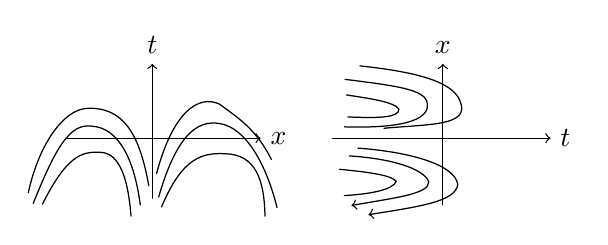
\begin{tikzpicture}[x=.90cm,y=.90cm,line cap=round,line width=.45pt]
\draw[->] (-1.20,0)--(1.53,0) node[right] {$x$};
\draw[->] (0,-.85)--(0,1.05) node[above] {$t$};
\draw (-1.75,-.77) .. controls (-1.60,-.08) and (-1.25,.40) .. (-.93,.42)
 .. controls (-.41,.45) and (-.18,.06) .. (-.05,-.67);
\draw (-1.68,-.92) .. controls (-1.36,-.12) and (-1.16,.21) .. (-.86,.17)
 .. controls (-.46,.15) and (-.25,-.33) .. (-.17,-.94);
\draw (-1.55,-.93) .. controls (-1.22,-.28) and (-1.02,-.18) .. (-.73,-.20)
 .. controls (-.45,-.21) and (-.34,-.60) .. (-.30,-1.10);
\draw (.06,-.50) .. controls (.29,.37) and (.65,.62) .. (.95,.48)
 .. controls (1.20,.29) and (1.46,.14) .. (1.68,-.30);
\draw (.09,-.83) .. controls (.36,.11) and (.68,.29) .. (1.02,.19)
 .. controls (1.39,.07) and (1.64,-.49) .. (1.76,-.98);
\draw (.13,-.97) .. controls (.42,-.28) and (.70,-.20) .. (1.03,-.22)
 .. controls (1.45,-.23) and (1.58,-.57) .. (1.59,-1.10);
\begin{scope}[shift={(4.1,0)}]
\draw[->] (-1.56,0)--(1.52,0) node[right] {$t$};
\draw[->] (0,-.94)--(0,1.05) node[above] {$x$};
\draw (-1.17,1.02) .. controls (-.42,.94) and (.13,.81) .. (.24,.53)
 .. controls (.40,.17) and (-.18,.20) .. (-.83,.14);
\draw (-1.38,.83) .. controls (-.67,.74) and (-.24,.69) .. (-.22,.49)
 .. controls (-.19,.31) and (-.42,.13) .. (-1.39,.16);
\draw (-1.36,.61) .. controls (-1.03,.56) and (-.68,.51) .. (-.62,.41)
 .. controls (-.62,.29) and (-.89,.28) .. (-1.34,.30);
\draw[->] (-1.20,-.14) .. controls (-.40,-.20) and (.17,-.39) .. (.21,-.65)
 .. controls (.19,-.90) and (-.37,-.97) .. (-1.05,-1.08);
\draw[->] (-1.32,-.25) .. controls (-.71,-.29) and (-.28,-.43) .. (-.20,-.61)
 .. controls (-.18,-.79) and (-.68,-.84) .. (-1.29,-.95);
\draw (-1.46,-.44) .. controls (-1.01,-.48) and (-.71,-.53) .. (-.66,-.61)
 .. controls (-.70,-.73) and (-1.04,-.79) .. (-1.39,-.81);
\end{scope}
\end{tikzpicture}}\endgroup
}
\end{GelfandAdjacentEvidence}
\begin{GelfandAdjacentEvidence}{GELFAND-P000999}{3}


Другое замеч. ур-е:
\begin{equation*}
\varepsilon\ddot u+\left(\frac{\dot u^3}{3}-\dot u\right)+u=0.
\tag{2}
\end{equation*}
(Рэлей)

Он сводится к ур-ю Ван-дер-Поля.

\SourceFigure{GELFAND-P000999}{jump-sketches}{Две кривые с вертикальными участками. У нижнего конца слева стрелка вниз. Короткий штрих у верхнего перегиба справа неясен.\par\smallskip
\begingroup\color{black}\GelfandFitDiagram{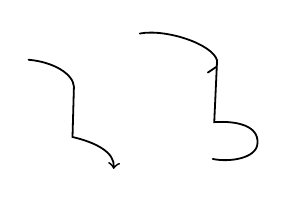
\begin{tikzpicture}[x=.9cm,y=.9cm,line cap=round,line width=.65pt]
\draw[->] (0,1.64) .. controls (.35,1.61) and (.63,1.44) .. (.64,1.26)
 --(.62,.55) .. controls (.96,.47) and (1.22,.33) .. (1.20,.10);
\draw (1.57,2.01) .. controls (1.94,2.08) and (2.60,1.86) .. (2.66,1.63)
 --(2.62,.76) .. controls (2.94,.78) and (3.25,.71) .. (3.23,.46)
 .. controls (3.22,.25) and (2.84,.19) .. (2.60,.24);
\draw (2.65,1.54)--(2.53,1.46);
\end{tikzpicture}}\endgroup
}
\end{GelfandAdjacentEvidence}
\begin{GelfandAdjacentEvidence}{GELFAND-P000999}{4}

[Справа, со стрелкой влево:] есть предельные реш. с такими скачками.
\SourceFigure{GELFAND-P000999}{jump-caption}{Стрелка от подписи направлена к двум кривым.}
\end{GelfandAdjacentEvidence}
\begin{GelfandAdjacentEvidence}{GELFAND-P000999}{5}


Ур-е (1) изучается с пом. нестандартного анализа!

$\Omega$ --- мн-во,
\[
F=2^\Omega,\qquad p:F\to(0,1).
\]
\SourceFigure{GELFAND-P000999}{probability-codomain}{Интервал написан с круглыми скобками: $(0,1)$.}
\end{GelfandAdjacentEvidence}
\begin{GelfandAdjacentEvidence}{GELFAND-P000999}{6}

\[
p(A\cup B)=p(A)+p(B)\quad\text{при }A\cap B=\varnothing.
\]
$X$ --- мн-во,
\[
x':\Omega\to X,\qquad x'':\Omega\to X.
\]
Случ. элемент $X$ --- класс эквивалентных отобр. $\Omega\to X$.

[Мелко под строкой:]
\[
x'\sim x''\Leftrightarrow P(x'=x'')=1.
\]
\SourceFigure{GELFAND-P000999}{equivalence-probability-symbol}{В условии эквивалентности написана прописная $P$.}
\end{GelfandAdjacentEvidence}


[Справа:] $x$ --- класс экв. $x'$. $\Rightarrow x'$ --- версия $x$.


\Needspace{7\baselineskip}
\begin{GelfandAdjacentEvidence}{GELFAND-P001000}{1}
\SourcePage{GELFAND-P001000}{unlabelled}
\underline{Числа Крускала:} простейший пример поля, расш. $\mathbb R$.
\SourceFigure{GELFAND-P001000}{surreal-heading}{В заголовке написано «Крускала».}
\end{GelfandAdjacentEvidence}

\[
\varnothing=0.
\]
\[
\begin{aligned}
\text{up}\quad&\uparrow=1,\\
\text{down}\quad&\downarrow=-1,\\
&\overbrace{\uparrow\uparrow\uparrow\ldots\uparrow}^{n}=n,\\
&\uparrow\downarrow=\frac12,\\
&\uparrow\downarrow\uparrow=\frac34.
\end{aligned}
\]

\begin{GelfandAdjacentEvidence}{GELFAND-P001000}{2}
(при изменении напр. шаг уменьш. вдвое)
\SourceFigure{GELFAND-P001000}{halving-rule}{Рукописная помета «при изменении напр. шаг уменьш. вдвое».}
\end{GelfandAdjacentEvidence}
\begin{GelfandAdjacentEvidence}{GELFAND-P001000}{3}


$\hat{\uparrow}$ --- беск. повторение $\uparrow$.
\[
\hat{\uparrow}\downarrow=\infty-1;\qquad
\hat{\uparrow}=\infty.
\]
[Перед $\infty-1$ зачёркнут знак.]
\Unclear{GELFAND-P001000}{infinity-cancelled-symbol}{Слева от $\infty$ штрихи закрывают зачёркнутый знак.}
\end{GelfandAdjacentEvidence}
\begin{GelfandAdjacentEvidence}{GELFAND-P001000}{4}

(нет предшествующего)
\begin{gather*}
\hat{\uparrow}\hat{\downarrow}=\frac12\infty.\\
\hat{\uparrow}:\hat{\uparrow}\hat{\downarrow}=2
\qquad\text{--- точная теор.}\\
\hat{\hat{\uparrow}}=\infty^2,\\
\uparrow\hat{\downarrow}=\varepsilon.
\end{gather*}
\SourceFigure{GELFAND-P001000}{iteration-hats}{В последней паре формул у первой стрелки две дуги, у направленной вниз стрелки --- одна.}
\end{GelfandAdjacentEvidence}
\begin{GelfandAdjacentEvidence}{GELFAND-P001000}{5}


\underline{Кричевер.}

([Зачёркнуто: неразборчиво] по (?) раб. Брозовского, Дзялошинского и Кричевера)
\Unclear{GELFAND-P001000}{krichever-intro-cancelled}{В начале скобки зачёркнута короткая запись.}
\end{GelfandAdjacentEvidence}
\begin{GelfandAdjacentEvidence}{GELFAND-P001000}{6}

\Unclear{GELFAND-P001000}{intro-preposition}{Между зачёркнутым и «раб.» предположительно «по».}
\end{GelfandAdjacentEvidence}
\begin{GelfandAdjacentEvidence}{GELFAND-P001000}{7}

\SourceFigure{GELFAND-P001000}{first-collaborator}{Фамилия в родительном падеже написана «Брозовского».}
\end{GelfandAdjacentEvidence}
\begin{GelfandAdjacentEvidence}{GELFAND-P001000}{8}

\[
G=\bigcup_n G_n,\qquad G_n\subset G_{n+1}.
\]
\Unclear{GELFAND-P001000}{group-chain-tail}{После $G_{n+1}$ стоит короткая запись, точное чтение не установлено.}
\end{GelfandAdjacentEvidence}
\begin{GelfandAdjacentEvidence}{GELFAND-P001000}{9}

\[
u(z),\qquad \Gamma\ni z.
\]
[Под $u(z)$, соединено чертой:] матричная ф-я.
 
[Под $\Gamma$, соединено чертой:] тор ($\mathbb C$/решётка).
\begin{gather*}
u^{ij}(z)=
\frac{\sigma(z-a_1^{ij})\ldots\sigma(z-a_n^{ij})}
{\sigma^n(z)}\,e^{\zeta(z)(x_i-x_j)},\\
a_1^{ij}+\ldots+a_n^{ij}=x_i-x_j.
\end{gather*}
\SourceFigure{GELFAND-P001000}{elliptic-exponent}{В показателе написано $\zeta(z)(x_i-x_j)$.}
\end{GelfandAdjacentEvidence}



\clearpage
\pdfbookmark[0]{Глава 21}{gelfand-archive-chapter-21}
\section*{Глава 21}
\Needspace{7\baselineskip}
\begin{GelfandAdjacentEvidence}{GELFAND-P001001}{1}
\SourcePage{GELFAND-P001001}{unlabelled}
\begin{center}$-\ \cdot\ -$\end{center}
\underline{\underline{8/II-82 г.}}\qquad\underline{Сем. Гельфанда}.

\underline{\underline{Müller Werner}}.

\underline{Lattice gravity}. (раб. с Cheeger и Schräder)
\SourceFigure{GELFAND-P001001}{collaborator-spelling}{В рукописи написано «Schräder».}
\end{GelfandAdjacentEvidence}
\begin{GelfandAdjacentEvidence}{GELFAND-P001001}{2}


1) Рассм. 1-мерн. мех. систему с гамильтонианом:
\begin{equation*}
H(p,q)=+\frac{p^2}{2m}+V(q)
\tag{1}
\end{equation*}
\[
q\to Q,\quad p\to P\qquad \text{операторы в }L^2(\mathbb R)
\]
\[
Qf(x)=xf(x),\qquad Pf(x)=i\hbar\frac{d}{dx}f(x)
\]
\SourceFigure{GELFAND-P001001}{momentum-sign}{В записи $Pf(x)$ перед $i\hbar$ нет знака минус.}
\end{GelfandAdjacentEvidence}
\begin{GelfandAdjacentEvidence}{GELFAND-P001001}{3}

\[
H(p,q)\to\widehat H
\]
Рассм. ур-е Шрёдингера
\begin{equation*}
i\frac{\partial}{\partial t}=\hbar^{-1}\widehat H f
\tag{2}
\end{equation*}
зад. эволюцию:
\begin{equation*}
f(x,t)=e^{-i\frac{t}{\hbar}\widehat H}f(x,0)
\tag{3}
\end{equation*}
\SourceFigure{GELFAND-P001001}{equation-two}{В (2) слева записано только $i\,\partial/\partial t$. Буква $f$ есть справа.}
\end{GelfandAdjacentEvidence}
\begin{GelfandAdjacentEvidence}{GELFAND-P001001}{4}


Вер. перехода из $x$ в $x'$ за время [над строкой вписано: от $t_0$ до] $t$ по Фейнману
\SourceFigure{GELFAND-P001001}{time-insertion}{Перед $t$ приписано «от $t_0$ до» со знаком вставки.}
\end{GelfandAdjacentEvidence}
\begin{GelfandAdjacentEvidence}{GELFAND-P001001}{5}

\begin{equation*}
\langle x'\mid e^{-i\frac{t}{\hbar}\widehat H}\mid x\rangle
=\int_{\substack{\text{по [вставлено: всем] путям }x\\x(0)=x,\ x(t)=x'}}
e^{-iS[x]}\prod_\tau\frac{dx(\tau)}{2\pi}
\tag{4}
\end{equation*}
\SourceFigure{GELFAND-P001001}{path-insertion}{«Всем» вписано над «по путям».}
\end{GelfandAdjacentEvidence}
\begin{GelfandAdjacentEvidence}{GELFAND-P001001}{6}

\begin{equation*}
S[x]=\int_0^t[\dot x^2(\tau)-V(x(\tau))]d\tau
\tag{5}
\end{equation*}
\SourceFigure{GELFAND-P001001}{action-normalization}{В (4) показатель $-iS[x]$. В (5) перед $\dot x^2(\tau)$ коэффициент не написан.}
\end{GelfandAdjacentEvidence}
\begin{GelfandAdjacentEvidence}{GELFAND-P001001}{7}

(см. посл. глава кн. Коноплевой и Попова)
\Unclear{GELFAND-P001001}{bibliography}{В ссылке читается «Коноплевой» без отчётливых точек над «е».}
\end{GelfandAdjacentEvidence}



\Needspace{7\baselineskip}
\begin{GelfandAdjacentEvidence}{GELFAND-P001002}{1}
\SourcePage{GELFAND-P001002}{4}
или: вместо $t$ вставить $t-t_0$

\hspace{2em}вместо $0$ --- '' --- $t_0$

\underline{М. Кас} придал нек-рый смысл инт. (4) с заменой $i\to1$
\begin{equation*}
\hbar\frac{\partial f}{\partial t}=\widehat H f,
\tag{6}
\end{equation*}
тогда
\begin{equation*}
\langle x'\mid e^{-\frac{t}{\hbar}Hx}\mid x\rangle
=\int_{\substack{\text{по всем путям}\\x:\,x(0)=x\\x(t)=x'}}
e^{-\int_0^t x(\tau)d\tau}\,dW(x)
\tag{7}
\end{equation*}
[Стрелка к $dW(x)$:] мера Винера.
\Unclear{GELFAND-P001002}{semigroup-exponent}{После $H$ видна буква $x$. Неясно, является ли она нижним индексом.}
\end{GelfandAdjacentEvidence}
\begin{GelfandAdjacentEvidence}{GELFAND-P001002}{2}

\SourceFigure{GELFAND-P001002}{heat-kernel}{В (6) справа перед $\widehat Hf$ нет минуса.}
\end{GelfandAdjacentEvidence}
\begin{GelfandAdjacentEvidence}{GELFAND-P001002}{3}

\SourceFigure{GELFAND-P001002}{heat-integrand}{В показателе под интегралом написано $x(\tau)$.}
\end{GelfandAdjacentEvidence}
\begin{GelfandAdjacentEvidence}{GELFAND-P001002}{4}


2) \underline{Гравитация}.
\[
i\mapsto1\qquad\rightsquigarrow
\]
[Зачёркнуто: «для» (?)] лоренц. метрика $\longmapsto$ риманова метрика.
\Unclear{GELFAND-P001002}{lorentz-cancellation}{Слово перед «лоренц.» зачёркнуто, предположительно «для».}
\end{GelfandAdjacentEvidence}
\begin{GelfandAdjacentEvidence}{GELFAND-P001002}{5}


$M$ --- компактное $C^\infty$-мн-зие
\[
\mathcal M=\{\text{пр-во всех рим. метрик на }M\}
\]
\[
G=\operatorname{Diff}(M)\quad\text{--- калибров. группа.}
\]
Действие [зачёркнуто: неразборчиво] [вписано ниже: Гильберта (-- Эйнштейна)]:
\begin{equation*}
S[g]=\lambda\int_M R\,d\operatorname{vol},\qquad
R\text{ --- скалярная кривизна}
\tag{8}
\end{equation*}
\Unclear{GELFAND-P001002}{action-cancellation}{После «Действие» прежняя запись зачёркнута. Ниже читается «Гильберта (-- Эйнштейна)».}
\end{GelfandAdjacentEvidence}
\begin{GelfandAdjacentEvidence}{GELFAND-P001002}{6}


(нетривиально: Эйнштейн считал, что действия нет)

--- в $R$ входят 2-е произв. $\Rightarrow$ ур-е \underline{a priori} 4-го порядка
\SourceFigure{GELFAND-P001002}{equation-order}{В конце строки написано «4-го порядка».}
\end{GelfandAdjacentEvidence}
\begin{GelfandAdjacentEvidence}{GELFAND-P001002}{7}


Но локально есть \underline{нековар. добавок} диверг. вида, [зачёркнуто: неразборчиво] не меняющий $S$.
\Unclear{GELFAND-P001002}{divergence-cancellation}{Чтение фразы под зачёркиванием после «вида» не установлено.}
\end{GelfandAdjacentEvidence}
\begin{GelfandAdjacentEvidence}{GELFAND-P001002}{8}


\underline{Задача (И.М.Г.)} Найти все комб. кривизн, где получ. ур-е меньшего порядка.

\underline{«Ответ»}: Эйнштейн и классы Понтрягина. \underline{Действие}:
\begin{equation*}
\int_{\mathcal M/G}e^{-S[g]-\text{æ}\operatorname{Vol}(M,g)}d\mu(g)
\tag{9}
\end{equation*}
\Unclear{GELFAND-P001002}{volume-coefficient}{Знак коэффициента перед $\operatorname{Vol}(M,g)$ похож на «æ». Возможно, это рукописное $\varkappa$.}
\end{GelfandAdjacentEvidence}
\begin{GelfandAdjacentEvidence}{GELFAND-P001002}{9}


\underline{Формально}:
\begin{equation*}
d\mu(g)=\prod_{x\in M}\det g(x)^{5/2}\prod_{\mu\leq\nu}dg_{\mu\nu}(x)
\tag{10}
\end{equation*}
\SourceFigure{GELFAND-P001002}{measure-exponent}{Показатель степени читается $5/2$, без знака минус.}
\end{GelfandAdjacentEvidence}
\begin{GelfandAdjacentEvidence}{GELFAND-P001002}{10}

(Фаддеев -- Попов)

Решёточная аппроксимация.

[Слева зачёркнут номер.]
\[
P^n\subset\mathbb R^N\qquad
P^n\underset{\varphi}{\longrightarrow}M\quad\text{триангуляция}
\]
[Черта от $P^n$ к подписи:] кусочно линейное подмн-зие.
\Unclear{GELFAND-P001002}{bottom-cancellation}{Под зачёркиванием предположительно «(11)».}
\end{GelfandAdjacentEvidence}



\Needspace{7\baselineskip}
\begin{GelfandAdjacentEvidence}{GELFAND-P001003}{1}
\SourcePage{GELFAND-P001003}{unlabelled}
Метрика на $M$ индуцирует кусочно-лин. метр. на $P$.
\[
(P,\ell),\qquad \ell:P^{(1)}\to\mathbb R_+
\]
(симп. $\rightsquigarrow$ его длина)

(11)
\SourceFigure{GELFAND-P001003}{polyhedron-sphere}{Подписи $P$, $\sigma^1$, $\varphi$, $M=S^2$. Пунктирные штрихи восстановлены по видимым участкам.\par\smallskip
\begingroup\color{black}\GelfandFitDiagram{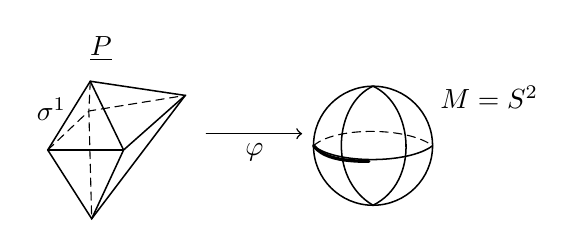
\begin{tikzpicture}[x=.9cm,y=.9cm,line cap=round,line width=.55pt]
\coordinate (top) at (.78,1.81);
\coordinate (west) at (.18,.84);
\coordinate (front) at (1.25,.84);
\coordinate (east) at (2.12,1.61);
\coordinate (low) at (.80,-.13);
\coordinate (rear) at (.76,1.39);
\draw[densely dashed,thin] (west)--(rear)--(east) (top)--(rear)--(low);
\draw (west)--(top)--(east)--(low)--cycle;
\draw (top)--(front)--(low) (west)--(front)--(east);
\node[above] at (.93,1.95) {\underline{$P$}};
\node[left] at (.58,1.41) {$\sigma^1$};
\draw[->] (2.42,1.07)--(3.77,1.07) node[midway,below] {$\varphi$};
\begin{scope}[shift={(4.77,.90)}]
\draw (0,0) circle (.84);
\draw (0,.84) .. controls (-.54,.60) and (-.65,-.46) .. (0,-.84);
\draw (0,.84) .. controls (.57,.58) and (.67,-.51) .. (0,-.84);
\draw[densely dashed,thin] (-.84,0) .. controls (-.54,.27) and (.48,.27) .. (.84,0);
\draw (-.84,0) .. controls (-.53,-.26) and (.50,-.26) .. (.84,0);
\draw[very thick] (-.84,0) .. controls (-.72,-.15) and (-.49,-.22) .. (-.06,-.22);
\node[right] at (.81,.69) {$M=S^2$};
\end{scope}
\end{tikzpicture}}\endgroup
}
\end{GelfandAdjacentEvidence}
\begin{GelfandAdjacentEvidence}{GELFAND-P001003}{2}


\underline{Дискр. версия $\displaystyle\int_M R\,d\operatorname{vol}$}.
\begin{equation*}
P^n\longrightarrow M\qquad\text{триангуляция}
\tag{12}
\end{equation*}
\[
\sigma^{n-2}\subset P^n
\]
$\delta(\sigma^{n-2})$ --- угловой дефект $\sigma^{n-2}$
\[
\sigma^n\supset\sigma^{n-2}
\]
$[\sigma^{n-2},\sigma^n]$ --- диэдральный угол
\begin{equation*}
\delta(\sigma^{n-2})=2\pi-\sum_{\sigma^n\supset\sigma^{n-2}}[\sigma^{n-2},\sigma^n]
\tag{13}
\end{equation*}
\begin{equation*}
R(P)=\sum_{\sigma^{n-2}\subset P}\delta(\sigma^{n-2})\operatorname{vol}(\sigma^{n-2})
\tag{14}
\end{equation*}
(Regge)

$P_n$ --- послед. триангуляций, $P_n\to M$
\begin{equation*}
\operatorname{mesh}(P_n)\underset{n\to\infty}{\longrightarrow}0
\tag{15}
\end{equation*}
\begin{equation*}
\underline{\text{Th.}}\quad\underline{\text{Тогда}}\quad
R(P_n)\underset{n\to\infty}{\longrightarrow}\int_M R\,d\operatorname{vol}
\tag{16}
\end{equation*}
Пока неясно, сходятся ли ур-я.

Барицентрич. подразделять не надо.
[Стрелка вверх к приписке:] углы стан. маленьк.
\SourceFigure{GELFAND-P001003}{skinny-simplex}{У внутренних штрихов показаны видимые соединения. Нижние линии частично наложены друг на друга.\par\smallskip
\begingroup\color{black}\GelfandFitDiagram{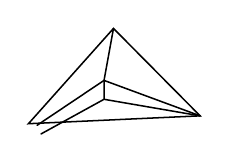
\begin{tikzpicture}[x=1cm,y=1cm,line cap=round,line width=.55pt]
\draw (0,0)--(1.08,1.21)--(2.18,.10)--cycle;
\draw (1.08,1.21)--(.96,.55)--(.96,.31);
\draw (.96,.55)--(.11,-.02) (.96,.55)--(2.18,.10);
\draw (.96,.31)--(.16,-.13) (.96,.31)--(2.18,.10);
\end{tikzpicture}}\endgroup
}
\end{GelfandAdjacentEvidence}
\begin{GelfandAdjacentEvidence}{GELFAND-P001003}{3}


\underline{Надо, чтобы углы были отделены от $0$}:
\SourceFigure{GELFAND-P001003}{midpoint-subdivision}{Отметки при вершинах переданы графически. Неясно, являются ли они буквами.\par\smallskip
\begingroup\color{black}\GelfandFitDiagram{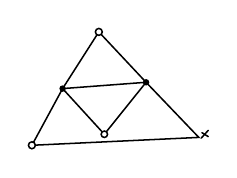
\begin{tikzpicture}[x=1cm,y=1cm,line cap=round,line width=.55pt]
\coordinate (a) at (0,0);
\coordinate (b) at (.85,1.44);
\coordinate (c) at (2.12,.10);
\coordinate (ab) at (.39,.72);
\coordinate (bc) at (1.45,.80);
\coordinate (ac) at (.92,.14);
\draw (a)--(ab)--(b)--(bc)--(c)--cycle;
\draw (ab)--(bc)--(ac)--cycle;
\draw[fill=white] (a) circle (.044) (b) circle (.044) (ac) circle (.041);
\fill (ab) circle (.041) (bc) circle (.041);
\draw (c) ++(.03,-.01)--++(.09,.10);
\draw (c) ++(.04,.06)--++(.08,-.05);
\end{tikzpicture}}\endgroup
}
\end{GelfandAdjacentEvidence}
\begin{GelfandAdjacentEvidence}{GELFAND-P001003}{4}

\underline{гладкая триангуляция берётся}. (существ. в раб. Мюллера о кручении Рэя -- Зингера)

\begin{center}$-\ \cdot\ -$\end{center}
\begin{equation*}
\int\operatorname{tr}(\Omega^k),\qquad \Omega\text{ --- тензор-кривизны}
\tag{17}
\end{equation*}
[Под $\Omega$ с чертой к нему:] 2-форма.
\[
\sigma^{n-2k}\subset P^n
\]
\begin{equation*}
\begin{aligned}
R_k(P^n)={}&\sum_{\sigma^{n-2k}\in P}\operatorname{vol}(\sigma^{n-2k})\,
\sum_{\sigma^{n-2k}\subset\sigma^{n-2\ell_1}\subset\cdots\subset\sigma^{n-2\ell_j}}
(-1)^j\\
&[\sigma^{n-2k},\sigma^{n-2\ell_1}]\ldots
[\sigma^{n-2\ell_{j-1}},\sigma^{n-2\ell_j}]
\end{aligned}
\tag{18}
\end{equation*}
[Над (18) наискось, со стрелкой влево вниз:] нормир. (?)
\SourceFigure{GELFAND-P001003}{formula-eighteen}{Последняя пара индексов в произведении читается $\ell_{j-1},\ell_j$.}
\end{GelfandAdjacentEvidence}
\begin{GelfandAdjacentEvidence}{GELFAND-P001003}{5}

\Unclear{GELFAND-P001003}{formula-note}{Приписка предположительно «нормир.», с неясными начальными штрихами.}
\end{GelfandAdjacentEvidence}



\Needspace{7\baselineskip}
\begin{GelfandAdjacentEvidence}{GELFAND-P001004}{1}
\SourcePage{GELFAND-P001004}{5}
$[\sigma^i,\sigma^{ij}]$ --- [вставлено сверху: \underline{нормализованный}] диэдральный угол (телесный)
[Стрелка к «телесный»:] нормируется на $1$.
\Unclear{GELFAND-P001004}{angular-indices}{Второй верхний индекс читается как $ij$, начальный штрих тонкий.}
\end{GelfandAdjacentEvidence}
\begin{GelfandAdjacentEvidence}{GELFAND-P001004}{2}


\begin{equation*}
\underline{\text{Th.}}\quad R_k(P_n)\longrightarrow\int_M\operatorname{tr}(\Omega^k) \tag{19}
\end{equation*}
$\Omega$ --- 2-форма со знач. в алг [зачёркнутый знак] матриц (матрица из 2-форм).
\Unclear{GELFAND-P001004}{omega-algebra}{Зачёркнутый знак, возможно $A$.}
\end{GelfandAdjacentEvidence}
\begin{GelfandAdjacentEvidence}{GELFAND-P001004}{3}

\begin{equation*}
\underline{k=n/2}\quad\Rightarrow\quad\text{получаем:}\quad\int\operatorname{tr}\Omega^k=\chi(M).
\end{equation*}
\Unclear{GELFAND-P001004}{euler-trace}{В рукописи стоит $\int\operatorname{tr}\Omega^k=\chi(M)$.}
\end{GelfandAdjacentEvidence}
\begin{GelfandAdjacentEvidence}{GELFAND-P001004}{4}

\begin{equation*}
\begin{aligned}
\chi(M)={}&\sum_{\sigma^0\subset\sigma^{2\ell_1}\subset\cdots\subset\sigma^{2\ell_j}}
(-1)^j[\sigma^0,\sigma^{2\ell_1}]\\
&\ldots[\sigma^{2\ell_{j-1}},\sigma^{2\ell_j}]
\end{aligned}\tag{20}
\end{equation*}
\Unclear{GELFAND-P001004}{euler-cancellation}{Неразборчивый зачёркнутый знак после первой закрывающей скобки.}
\end{GelfandAdjacentEvidence}
\begin{GelfandAdjacentEvidence}{GELFAND-P001004}{5}

Что-то похожее есть в раб. \underline{Брина}, рассказ. на семинаре $\sim1946$ г., неизвестно, что оно даёт в пределе.

$\displaystyle\int_M\operatorname{tr}(\Omega^k)$ опред. так: домножаем $\operatorname{tr}(\Omega^k)$ на стандартную [зачёркнуто: форму?] форму ([вставлено сверху: инвар.] полином от кривизны).
\Unclear{GELFAND-P001004}{standard-form-cancellation}{Зачёркнутое слово предположительно «форму».}
\end{GelfandAdjacentEvidence}
\begin{GelfandAdjacentEvidence}{GELFAND-P001004}{6}

\begin{equation*}
\mathcal M(P^n)=\{\text{пр-во всех кус.-лин. метрик на }P^n\}\tag{21}
\end{equation*}
$\sigma^n\subset\mathbb R^N$ \(\xrightarrow{\quad}\) $n$-мерн. симплекс

\SourceFigure{GELFAND-P001004}{tetrahedron}{Вершины $0,1,2,3$, подписаны рёбра $\ell_{01}$ и $\ell_{03}$.\par\smallskip
\begingroup\color{black}\GelfandFitDiagram{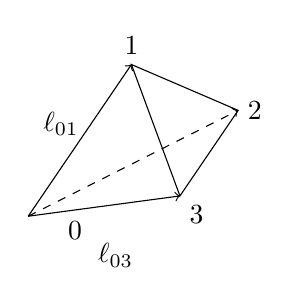
\begin{tikzpicture}[scale=1.12]
\coordinate (v0) at (0,0);
\coordinate (v1) at (1.17,1.72);
\coordinate (v2) at (2.38,1.2);
\coordinate (v3) at (1.72,0.23);
\draw[->] (v0) -- (v1);
\draw (v1) -- (v2) -- (v3) -- cycle;
\draw[->] (v0) -- (v3);
\draw[dashed,->] (v0) -- (v2);
\node[below] at (0.53,0.05) {$0$};
\node[above] at (v1) {$1$};
\node[right] at (v2) {$2$};
\node[below right] at (v3) {$3$};
\node[above left] at (0.68,0.8) {$\ell_{01}$};
\node[below] at (0.99,-0.2) {$\ell_{03}$};
\end{tikzpicture}}\endgroup
}
\end{GelfandAdjacentEvidence}
\begin{GelfandAdjacentEvidence}{GELFAND-P001004}{7}


\[
\ell\rightsquigarrow g=(g_{ij}),\qquad
g_{ij}=\frac12(\ell_{0i}^2+\ell_{0j}^2-\ell_{ij}^2)
\]
\begin{flushright}\underline{симметр. и положит. определена}\end{flushright}
\[
\mathcal P=\{\text{симм. полож. опр. матрицы }n\times n\}
\]
'' $GL(n)/O(n)$
\[
\mathcal M(\sigma^n)\equiv GL(n)/O(n)
\]
\underline{Инвар. мера на $\mathcal M(\sigma^n)$}:
\begin{equation*}
\frac{1}{\det g^{\frac{n+1}{2}}}\prod_{i\le j}dg_{ij}\tag{22}
\end{equation*}
\begin{equation*}
\frac{1}{\operatorname{vol}(\sigma^n,\ell)^{n+1}}\prod d\ell_{ij}\tag{23}
\end{equation*}
--- мера на $\mathcal M(\sigma^n)$ (другой способ записи).
\Unclear{GELFAND-P001004}{measure-change}{В (23) рукопись даёт $\prod d\ell_{ij}$.}
\end{GelfandAdjacentEvidence}
\begin{GelfandAdjacentEvidence}{GELFAND-P001004}{8}

\begin{equation*}
\prod_{x\in M}\operatorname{deg}g(x)^{5/2}\prod_{\mu\le\nu}dg_{\mu\nu}\tag{24}
\end{equation*}
\Unclear{GELFAND-P001004}{last-measure}{Конечный штрих в «deg» спускается под строку, в отличие от «det» в (22). Показатель в (24) записан как $5/2$.}
\end{GelfandAdjacentEvidence}



\Needspace{7\baselineskip}
\begin{GelfandAdjacentEvidence}{GELFAND-P001005}{1}
\SourcePage{GELFAND-P001005}{unlabelled}
\begin{equation*}
\mathcal M(P^n)\hookrightarrow\prod_{\sigma^n\subset P^n}\mathcal M(\sigma^n) \tag{25}
\end{equation*}
(подмн-зие)

Возникает индуц. [зачёркнуто в строке: метрика?] [над строкой обведено и зачёркнуто: кривизна?] [снизу обведено: метрика] на $\mathcal M(P^n)$ [зачёркнуто справа: не удовлетворяющ…].
\Unclear{GELFAND-P001005}{metric-cancel-main}{В строке предположительно «метрика», большая часть слова зачёркнута.}
\end{GelfandAdjacentEvidence}
\begin{GelfandAdjacentEvidence}{GELFAND-P001005}{2}

\Unclear{GELFAND-P001005}{metric-cancel-upper}{Обведённое и зачёркнутое слово над строкой может читаться «кривизна» или «метрика».}
\end{GelfandAdjacentEvidence}
\begin{GelfandAdjacentEvidence}{GELFAND-P001005}{3}

\Unclear{GELFAND-P001005}{right-cancellation}{Под зачёркиванием читается «не удовлетворяющ…». Окончание и следующие штрихи не установлены.}
\end{GelfandAdjacentEvidence}


($\rightsquigarrow$ усл. склеивания)

Вводится мера на пр-ве всех метризаций. $\Rightarrow$ объём, индуцированный рим. метрикой.
\[
P_n\underset{n\to\infty}{\longrightarrow}M
\]
(На $\mathcal M(\sigma^n)$ инвар. метрика как на симметрич. пр-ве.)

\underline{Идея}: $M^n\subset E^N$ \underline{изометрич.}

Кинематич. ф-ла Чженя:
\[
k=N-n+2,
\]
$\mathcal G_{N,k}$ = афф. грассманиан $E^k\subset E^N$

$dE^k$ --- мера на $\mathcal G_{N,k}$
\begin{equation*}
\int_{E^k\in\mathcal G_{N,k}}\chi(M^n\cap E^k)\,dE^k
=c_{N,k}\int_M R\,d\operatorname{vol} \tag{26}
\end{equation*}
\begin{equation*}
\int_{\mathcal G_{N,k}}\chi(P^n\cap E^k)\,dE^k
=c_{N,k}R(P^n) \tag{27}
\end{equation*}
[Под $P^n$ с вертикальной чертой:] симплиц. подмн-зие

[Под правой частью:] (комбинат. скал. кривизна)
\[
P_n\longrightarrow M
\]
подинтегр. ф-и в (26) и (27) будут п.в. совпадать.

\begin{GelfandAdjacentEvidence}{GELFAND-P001005}{4}
\begin{center}--- . ---\end{center}
Для $\displaystyle\int\operatorname{tr}(\Omega^k)$, $k=N-n+2\ell$
\begin{equation*}
\int_{E^k\in\mathcal G_{N,k}}\chi(M^n\cap E^k)\,dE^k
=c_{N,k}\int_M\operatorname{tr}(\Omega^\ell) \tag{28}
\end{equation*}
\Unclear{GELFAND-P001005}{curvature-exponent}{В строке перед (28) написано $\Omega^k$, в правой части (28) написано $\Omega^\ell$.}
\end{GelfandAdjacentEvidence}

\begin{equation*}
\underset{\text{лев. ч. (27)}}{\text{--- '' ---}}=c_{N,k}R_\ell(P^n). \tag{29}
\end{equation*}


\Needspace{7\baselineskip}
\begin{GelfandAdjacentEvidence}{GELFAND-P001006}{1}
\SourcePage{GELFAND-P001006}{6}
\underline{15/II-82}\qquad \underline{Сем. Гельфанда}

\underline{Гинзбург.}

$M$ --- симпл. мн-зие

($\omega$ --- соотв. 2-форма)

$A$ --- группа, действ. на $M$ гамильтоновым образом.

1) $A$ сохраняет $\omega$

$\xi\in\mathfrak A$ --- соотв. алгебра Ли

$\xi\longrightarrow\omega(\xi,\cdot)$ глобально (?) точна; точна:
\Unclear{GELFAND-P001006}{exactness-word}{Слово перед «точна» предположительно «глобально» по высокой петле в середине. Возможно «локально».}
\end{GelfandAdjacentEvidence}
\begin{GelfandAdjacentEvidence}{GELFAND-P001006}{2}


2) $\mathfrak A\ni a\longmapsto H_a$\quad (гамильтониан)

гомоморфизм алгебр Ли.

\underline{отобр. момента}: $\mu\colon M\longrightarrow\mathfrak A^*$
\[
m\longmapsto\mu(m),\qquad
\mu(m)(\underset{\substack{\uparrow\\\mathfrak A}}{a})=H_a(m)
\]
\SourceFigure{GELFAND-P001006}{moment-map-argument}{Стрелка от $\mathfrak A$ снизу указывает на аргумент $a$.}
\end{GelfandAdjacentEvidence}


Перестанов. с действием $A$ и согл. со скобкой Пуассона.

\begin{flushright}[Две короткие наклонные черты.]\end{flushright}


\Needspace{7\baselineskip}
\begin{GelfandAdjacentEvidence}{GELFAND-P001007}{1}
\SourcePage{GELFAND-P001007}{unlabelled}
\underline{22/II-82~г.}\qquad \underline{Сем. Гельфанда}

\underline{Арнольд.}

\[
V(\varepsilon)=\sum_{i=0}^{n}V_k\varepsilon^k,\qquad
\sigma_i(k)=\sum_{C_n^i}k_1\ldots k_i
\]
[Под $V(\varepsilon)$:] объём ($\varepsilon$-оболочка вып. тела). \quad (Теорема Минковского --- это многочлен.)
\Unclear{GELFAND-P001007}{summation-index}{Внизу суммы написано $i=0$, а в слагаемом $V_k\varepsilon^k$.}
\end{GelfandAdjacentEvidence}
\begin{GelfandAdjacentEvidence}{GELFAND-P001007}{2}


\[
k_s\text{ --- соб. числа }\frac{2\ \text{кв. ф.}}{1\ \text{кв. ф.}}
\]
\[
V_i=C_i\int_{\partial D}\sigma_i(k)\,dS
\]
[Под $C_i$ короткая вертикальная черта.]
\[
V_k=\widetilde C_k
\underbrace{\int_{\xi\in G_{n,k}}\operatorname{mes}(\pi_\xi D)\,d\xi}_{\text{''}},
\qquad \pi_\xi\colon \mathbb R^n\longrightarrow\xi
\]
\[
\int_{H_{n,k}}\chi(h\cap D)\,dh
\]
\SourceFigure{GELFAND-P001007}{integral-link}{Под верхним интегралом скобка с поднятыми концами и две короткие косые черты.}
\end{GelfandAdjacentEvidence}
\begin{GelfandAdjacentEvidence}{GELFAND-P001007}{3}


$H_{n,k}$ --- все плоск., не обязательно прох. через $0$

$\chi$ --- эйлерова хар-ка.

\underline{Это способ} [зачёркнуто: Бюф\ldots] \underline{Бюффона} (и потом обобщил Сантало)
[Под словами «способ Бюффона»:] вычисления числа $\pi$.
\Unclear{GELFAND-P001007}{buffon-cancellation}{В зачёркнутой записи различимы начальные штрихи «Бюф\ldots».}
\end{GelfandAdjacentEvidence}
\begin{GelfandAdjacentEvidence}{GELFAND-P001007}{4}


Вычисление констант $C_k$, $\widetilde C_k$ --- с помощью шаров.

\underline{Переносится на решётчатый случай.}

Вместо объёма --- число целых точек.

\underline{целочисл. параллелограм} (\ldots липед?)
\Unclear{GELFAND-P001007}{parallelogram-caption}{После точек в скобках читается предположительно «липед».}
\end{GelfandAdjacentEvidence}
\begin{GelfandAdjacentEvidence}{GELFAND-P001007}{5}


\SourceFigure{GELFAND-P001007}{parallelogram-diagram}{Нижняя сторона продолжена пунктиром. У правой нижней вершины петля. Неясно, является ли она отдельным знаком $0$.\par\smallskip
\begingroup\color{black}\GelfandFitDiagram{\begin{tikzpicture}[x=.75cm,y=.75cm,line width=.45pt]
\coordinate (a) at (0,0);
\coordinate (b) at (1.8,.9);
\coordinate (c) at (2.72,2.73);
\coordinate (d) at (.92,1.83);
\draw (a)--(b)--(c)--(d)--cycle;
\draw[dashed] (-1.42,-.71)--(a) (b)--(3.8,1.9);
\fill (a) circle (1.5pt) (b) circle (1.5pt)
      (c) circle (1.5pt) (d) circle (1.5pt);
\draw (1.76,.91) to[out=220,in=230] (1.81,.79) to[out=50,in=275] (1.86,.92);
\end{tikzpicture}}\endgroup
}
\end{GelfandAdjacentEvidence}
\begin{GelfandAdjacentEvidence}{GELFAND-P001007}{6}


Объём параллелепипеда --- число, показ., сколько элемент. пар.-липедов.

На прямой возникает решётка из пересечений.

Надо взять факторпр-во и это даёт аналог высоты.

(там тоже есть аналог решётки)

\underline{Mac Mullen} доклад в [зачёркнуто: Ванку\ldots] Ванкувере --- там есть лит-ра.
\Unclear{GELFAND-P001007}{vancouver-cancellation}{Первое написание зачёркнуто. Читается «Ванку\ldots».}
\end{GelfandAdjacentEvidence}
\begin{GelfandAdjacentEvidence}{GELFAND-P001007}{7}


\underline{И. М. Гельфанд.}

\underline{О книге Mc Donald'а} «Симметрические ф-и и полиномы Холла»

\underline{Задача.} Рассм. разбиение (partition)
\[
(L)\qquad \lambda_1\geq\lambda_2\geq\ldots\geq\lambda_k
\qquad (\text{целые числа})
\]
Разреш. дописывать нули.

Способы записи: $(L)$ или
\[
\begin{array}{rccccc}
5&\bullet&\bullet&\bullet&\bullet&\bullet\\
4&\bullet&\bullet&\bullet&\bullet&\\
4&\bullet&\bullet&\bullet&\bullet&\\
1&\bullet&&&&
\end{array}
\]
Вместо точек --- квадратики лучше (схемы Юнга).

\SourceFigure{GELFAND-P001007}{young-diagram}{Ряды из $5,4,4,1$ клеток в пунктирной рамке с отметками $m$ и $n$.\par\smallskip
\begingroup\color{black}\GelfandFitDiagram{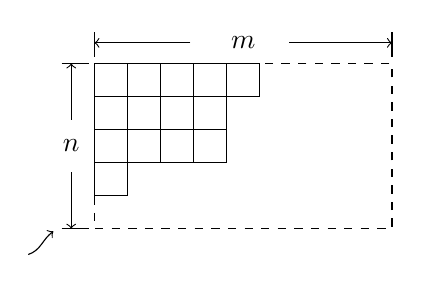
\begin{tikzpicture}[x=.42cm,y=.42cm,line width=.4pt]
\draw[dashed] (0,0) rectangle (9,-5);
\draw (0,0)--(5,0)--(5,-1)--(4,-1)--(4,-3)--(1,-3)--(1,-4)--(0,-4)--cycle;
\draw (0,-1)--(4,-1) (0,-2)--(4,-2) (0,-3)--(1,-3);
\draw (1,0)--(1,-3) (2,0)--(2,-3) (3,0)--(3,-3) (4,0)--(4,-1);
\draw (0,.2)--(0,.96) (9,.2)--(9,.96);
\draw[->] (2.9,.62)--(0,.62);
\draw[->] (5.9,.62)--(9,.62);
\node at (4.5,.62) {$m$};
\draw (-.99,0)--(-.15,0) (-.99,-5)--(-.15,-5);
\draw[->] (-.7,-1.7)--(-.7,0);
\draw[->] (-.7,-3.3)--(-.7,-5);
\node at (-.7,-2.5) {$n$};
\draw[->] (-2,-5.78) to[out=18,in=216] (-1.24,-5.08);
\end{tikzpicture}}\endgroup
}
\end{GelfandAdjacentEvidence}


Поместим в пр-к размерами $m\times n$ и рассм. числа


\Needspace{7\baselineskip}
\begin{GelfandAdjacentEvidence}{GELFAND-P001008}{1}
\SourcePage{GELFAND-P001008}{11}
\[
(*)\quad\left\{
\begin{array}{ll}
\lambda_i+n-i,&1\leq i\leq n,\\
n-1+j-\lambda'_j,&1\leq j\leq m
\end{array}\right.
\]

$\lambda'=4,3,3,3,1$ --- двойств. картинка

\underline{Задача:}

Набор из $m+n$ чисел $(*)$ --- перестановка чисел $0,1,2,\ldots,m+n-1$.

\underline{Следствие.}
\[
f_{\lambda,n}(t)\overset{\mathrm{def}}{=}\sum_{i=1}^{n}t^{\lambda_i+n-i}
\]
Тогда
\[
f_{\lambda,n}(t)+t^{m+n-1}f_{\lambda,m}(t)=\frac{1-t^{m+n}}{1-t}
\]
\Unclear{GELFAND-P001008}{generating-function}{Во втором слагаемом написано $f_{\lambda,m}(t)$, без видимого штриха у $\lambda$ и без обратного аргумента.}
\end{GelfandAdjacentEvidence}
\begin{GelfandAdjacentEvidence}{GELFAND-P001008}{2}


\underline{И. М. Гельфанд} с раб. \underline{Гийемина}
\Unclear{GELFAND-P001008}{author-name}{Фамилия предположительно читается «Гийемина».}
\end{GelfandAdjacentEvidence}
\begin{GelfandAdjacentEvidence}{GELFAND-P001008}{3}


\underline{Новые усл-ия асимпт. ф-лы Вейля}

\underline{Симпл. конус:}\qquad $\rho_a^*\omega=a\omega$,\quad $a>0$.

\underline{Пример 1.} $\mathbb R^{2n}=\{(x,\xi)\}$,
$x\in\mathbb R^n$, $\xi\in(\mathbb R^n)^*$,
$\rho_a(x,\xi)=(a^{1/2}x,a^{1/2}\xi)$.

\underline{Пример 2.} $T^*X$\qquad $a(x,\xi)=(x,a\xi)$.
\Unclear{GELFAND-P001008}{cotangent-base}{Основание после $T^*$ густо переписано, предположительно $X$.}
\end{GelfandAdjacentEvidence}
\begin{GelfandAdjacentEvidence}{GELFAND-P001008}{4}


\underline{Арнольд.}

Локально все конусы одинаковы: фактор --- контактное мн-зие.

(Симпл. конусы $\Longleftrightarrow$ конт. мн-зия)

Квантование надо именно контактное, т.к. надо действие --- \underline{1-форму!!}
\Unclear{GELFAND-P001008}{contact-ending}{Окончание слова после «именно» читается предположительно как «контактное».}
\end{GelfandAdjacentEvidence}
\begin{GelfandAdjacentEvidence}{GELFAND-P001008}{5}


\underline{Утв.} Всегда квантуется и единственным обр. стр. алг. Вейля, микролокально единств. и топол. (микролокально) классич. алг. Вейля.
\Unclear{GELFAND-P001008}{construction-abbreviation}{Перед «алг. Вейля» читается «стр.».}
\end{GelfandAdjacentEvidence}
\begin{GelfandAdjacentEvidence}{GELFAND-P001008}{6}


\underline{Квантование} --- [зачёркнуто: набор\ldots]
\Unclear{GELFAND-P001008}{quantization-cancellation}{В зачёркнутой строке читается начало «набор\ldots».}
\end{GelfandAdjacentEvidence}
\begin{GelfandAdjacentEvidence}{GELFAND-P001008}{7}


\[
x_k\longmapsto x_k,\qquad \xi_k\longmapsto i\frac{\partial}{\partial x_k}.
\]
\Unclear{GELFAND-P001008}{quantization-convention}{В образе $\xi_k$ стоит $i$ без минуса.}
\end{GelfandAdjacentEvidence}
\begin{GelfandAdjacentEvidence}{GELFAND-P001008}{8}

\[
p(x,\xi)=\sum_{i=0}^{\infty}p_i(x,\xi),\qquad
p_i\text{ --- однор. степ. }2\mu-2i
\]
\[
\rho_a(x,\xi)=(a^{1/2}x,a^{1/2}\xi);\qquad \mu\in\mathbb C.
\]
(Это символ порядка $\mu$).
\[
(Pf)(x)=(2\pi)^{-n}\int p\left(\frac{x+y}{2},\xi\right)
  e^{i\xi\cdot(x-y)}u(y)\,dy\,d\xi
\]
\Unclear{GELFAND-P001008}{kernel-function}{В левой части стоит $(Pf)(x)$, а под интегралом $u(y)$.}
\end{GelfandAdjacentEvidence}
\begin{GelfandAdjacentEvidence}{GELFAND-P001008}{9}


$W^\mu$ --- пр-во таких операторов,\qquad $\underline{W^{\mu-1}\subset W^\mu}$.

\underline{Символ:} элемент $W^\mu/W^{\mu-1}$.

$H$ --- гильб. пр-во, $S$ --- плотное подпр-во, где действ. все такие опер..

$\underline W^\mu$ --- соотв. пр-во опер.
(вида $A_1+\cdots+A_k$, $A_i\in W^{\mu_i}$ в примере).
\Unclear{GELFAND-P001008}{w-subscript}{Под $W$ перечёркнутые петлеобразные штрихи. Чтение индекса не установлено.}
\end{GelfandAdjacentEvidence}


\underline{Аксиомы:}
\[
\substack{\text{группа}\\ A}
\quad\left\lceil
\begin{aligned}
1)\quad &\underline W^\mu\supset\underline W^{\mu-1}\\
2)\quad &A\in\underline W^\mu,\quad B\in\underline W^\nu
 \ \Longrightarrow\ AB\in\underline W^{\mu+\nu}\\
3)\quad &A\in\underline W^\mu,\quad B\in\underline W^\nu
 \ \Longrightarrow\ [A,B]\in\underline W^{\mu+\nu-1}\\
4)\quad &A\in\underline W^\mu\ \Longrightarrow\ A^*\in\underline W^{\bar\mu}
\end{aligned}\right.
\]
\[
5)\quad I\in\underline W^0
\]


\Needspace{7\baselineskip}
\begin{GelfandAdjacentEvidence}{GELFAND-P001009}{1}
\SourcePage{GELFAND-P001009}{unlabelled}
\[
\left\lfloor
\begin{aligned}
6)\quad&\forall A_i\in\underline W^{\mu-i},\quad i=0,1,2,\ldots\\
&\Longrightarrow\ \exists A\in\underline W^\mu,\qquad
A-\sum_{i=0}^{N-1}A_i\in\underline W^{\mu-N}.
\end{aligned}\right.
\]
\SourceFigure{GELFAND-P001009}{asymptotic-bracket}{Слева от пункта 6) нижний конец квадратной скобки.}
\end{GelfandAdjacentEvidence}
\begin{GelfandAdjacentEvidence}{GELFAND-P001009}{2}


\underline{Группа $B$.}

$1^{\circ}$. Если $\operatorname{Re}\mu\leq0$, то $\forall A\in\underline W^\mu$ ограничен.

$2^{\circ}$. Если $\operatorname{Re}\mu<0$, то $\forall A\in\underline W^\mu$ компактен.

$3^{\circ}$. $\exists s_0>0$, если $A\in\underline W^\mu$,
$\operatorname{Re}\mu<-s_0$; то $A$ ядерный.

\underline{Группа $C$.}
\[
A\in\underline W^0,\quad A\text{ компактен}
\ \Longrightarrow\ A\in\underline W^{-1}
\]

\underline{$D$.} Точная посл.

\SourceFigure{GELFAND-P001009}{exact-sequence}{Подчёркивания $W$ и стрелки прямой последовательности.\par\smallskip
\begingroup\color{black}\GelfandFitDiagram{\begin{tikzcd}[ampersand replacement=\&,column sep=small]
0\arrow[r]\&\underline W^{\mu-1}\arrow[r]\&\underline W^\mu\arrow[r]\&
\underline W^\mu/\underline W^{\mu-1}\arrow[r]\&0
\end{tikzcd}}\endgroup
}
\end{GelfandAdjacentEvidence}


«хорошо» разлож. в прямую сумму.

\underline{$E$.}\qquad $\exists A(\mu)\in\underline W^\mu$, аналит. завис. от $\mu\in\mathbb C$,
такой что $A(0)-I\in\underline W^{-1}$ и
\[
A(\mu)A(\nu)-A(\nu+\mu)\in\underline W^{\mu+\nu-1}.
\]


\Needspace{7\baselineskip}
\begin{GelfandAdjacentEvidence}{GELFAND-P001010}{1}
\SourcePage{GELFAND-P001010}{15}
\underline{\underline{1/III-82.}}\qquad \underline{Сем. Гельфанда.}

\underline{R. MacPherson.}\quad \underline{The title of a paper}
[зачёркнуто: which?] \underline{he would speak about:}
\Unclear{GELFAND-P001010}{title-cancellation}{Зачёркнутое английское слово предположительно «which».}
\end{GelfandAdjacentEvidence}
\begin{GelfandAdjacentEvidence}{GELFAND-P001010}{2}


\SourceFigure{GELFAND-P001010}{title-diagram}{«Holonomes» и «char variety» набраны в написании источника. Волнистая и пунктирная стрелки ведут к нижней подписи.\par\smallskip
\begingroup\color{black}\GelfandFitDiagram{\begin{tikzpicture}[x=.80cm,y=.67cm,font=\small]
\node (p) at (0,0) {\underline{Perverse Sheaves}};
\node at (2.30,0) {$\approx$};
\node (h) at (5.03,0) {\underline{Holonomes $\mathcal D$-modules}};
\node[font=\scriptsize] at (-.49,-.58) {(извращенные ?)};
\node[font=\scriptsize] at (-.25,-1.20) {(катег.};
\node (v) at (5.0,-2.14) {char variety};
\draw[dashed,->] (.79,-.53)--(v.west);
\node at (1.65,-1.77) {?};
\draw[->] (h.south) to[out=275,in=85] (5.03,-.64)
 to[out=265,in=85] (4.98,-.91) to[out=275,in=100] (5.03,-1.20)
 to[out=270,in=83] (v.north);
\end{tikzpicture}}\endgroup
}
\end{GelfandAdjacentEvidence}
\begin{GelfandAdjacentEvidence}{GELFAND-P001010}{3}


\underline{Другой заголовок:}

$H(X\longrightarrow Y)$\qquad \underline{теория гомол. отображений пр-в.}
\begin{align*}
H(X\longrightarrow pt)&=H_*(X)\\
H(X\overset{\mathrm{id}}{\longrightarrow}X)&=H^*(X)
\end{align*}

\SourceFigure{GELFAND-P001010}{composition-diagram}{Нижняя дуга направлена от $X$ к $Z$.\par\smallskip
\begingroup\color{black}\GelfandFitDiagram{\begin{tikzcd}[ampersand replacement=\&]
X\arrow[r]\arrow[rr,bend right=25]\&Y\arrow[r]\&Z
\end{tikzcd}}\endgroup
}

\underline{есть умножение}, накрыв. композ. отобр.
\end{GelfandAdjacentEvidence}
\begin{GelfandAdjacentEvidence}{GELFAND-P001010}{4}

\underline{D. McDuff.}\qquad \underline{Когом. группы диффеом., сохр. объём.}

\[
\mathcal G=\operatorname{Diff}_{\omega 0}^{c}M,
\]
$\omega$ --- форма объёма на $M$, $M$ --- мн-зие;

$c$ --- с комп. носителем; $0$ --- связная компонента $Id$.

$\mathcal G$ с обычной топологией $(C^\infty)$.

$G$ --- та же гр. в дискр. топ.
\[
G\underset{\text{тожд.}}{\longrightarrow}\mathcal G
\]
\[
\bar B\mathcal G\longrightarrow
\overset{\substack{K(G,1)\\\shortparallel}}{BG}
\longrightarrow B\mathcal G
\qquad (\text{классиф. пр-ва})
\]
\SourceFigure{GELFAND-P001010}{classifying-spaces}{Над $BG$ написано $K(G,1)$ с двумя короткими чертами. От $\bar B\mathcal G$ штрих ведёт к подписи о слое.}
\end{GelfandAdjacentEvidence}
\begin{GelfandAdjacentEvidence}{GELFAND-P001010}{5}

гомот. слой (превр. отобр. в расслоение, тогда $\bar B\mathcal G$ --- слой)

$\bar B\mathcal G$ зав. только от окр. $1$ в $\mathcal G$.

Это топологич. версия алг. Ли в нек-ром смысле.

\underline{Фукс:}
\[
G/H\longrightarrow BH\longrightarrow BG
\]
(обычно); если $H$ [вставлено сверху: очень] плотно в $G$, то фунд. область --- «инфинитезим.» окр. единицы.

$\bar B\mathcal G\times M$ имеет слоение $\mathcal F$,
трансверс. ко всем слоям $x\times M$
и определяемое [вставлено сверху: такой] замкнутой $n$-формой $\Omega$, что $\Omega|_{x\times M}=\omega$.
\Unclear{GELFAND-P001010}{closed-form-overwriting}{В окончании «замкнутой» есть густо переписанные штрихи.}
\end{GelfandAdjacentEvidence}
\begin{GelfandAdjacentEvidence}{GELFAND-P001010}{6}


\SourceFigure{GELFAND-P001010}{bundle-diagram}{В нижней левой подписи читается $\bar BG$, а в верхней $\bar B\mathcal G$. Знак произведения вверху слит со штрихами $M$. Над правым $M$ густо зачёркнутая запись.\par\smallskip
\begingroup\color{black}\GelfandFitDiagram{\begin{tikzcd}[ampersand replacement=\&,column sep=small]
E'\cong\bar B\mathcal G\times M\arrow[d]\&E'\arrow[d,"M"]\&E\arrow[d,"M"]\\
\bar B G\arrow[r]\&BG\arrow[r]\&B\mathcal G
\end{tikzcd}}\endgroup
}
\end{GelfandAdjacentEvidence}
\begin{GelfandAdjacentEvidence}{GELFAND-P001010}{7}


$E$ --- станд. расслоение со слоем $M$.

$E'$ --- его подъём, [зачёркнуто: связность?] у него $0$-я кривизна,
т.к. слой соотв. главного рассл. дискретен.
\Unclear{GELFAND-P001010}{connection-cancellation}{В зачёркнутом слове видно начальное «с», предположительно «связность».}
\end{GelfandAdjacentEvidence}


Слева --- огранич. на слой --- оно стан. трив. по св-ву классиф. пр-ва.

Связн. $0$-й кривизны переносится и даёт слоение на $\bar B\mathcal G\times M$


\Needspace{7\baselineskip}
\begin{GelfandAdjacentEvidence}{GELFAND-P001011}{1}
\SourcePage{GELFAND-P001011}{unlabelled}
$\Omega-\pi^*\omega=0$ вблизи $\infty$ на $M$.

Классы.
\[
c_k(M)\in H^k\left(\bar B\operatorname{Diff}^{c}_{\omega_0}M;
\underset{\substack{\vert\\\text{коэффициенты}}}{H_c^{n-k}(M;\mathbb R)}\right)
\]
$n=\dim M$.

Пусть $K$ --- $k$-цикл в $\bar B\operatorname{Diff}^{k}_{\omega_0}M$.
\Unclear{GELFAND-P001011}{upper-diff-superscript}{В определении цикла над $\operatorname{Diff}$ стоит $k$, в соседних формулах стоит $c$.}
\end{GelfandAdjacentEvidence}
\begin{GelfandAdjacentEvidence}{GELFAND-P001011}{2}

\[
c_k(M)(K)=\text{класс замкнутой }(n-k)\text{-формы }
 x\longmapsto\int_{K\times x}\Omega
\]

\underline{Пример.} $M=T^n$, $K=T^n$.
\[
\begin{aligned}
T^n\times T^n&\longrightarrow T^n\\
(x,y)&\longmapsto x+y
\end{aligned}
\]
Берем [зачёркнуто: слоение на $T^n$ и поднимем?] [вставлено сверху в выноске: возник. слоение]
на $T^n\times T^n$. Получ. слоение, предст. цикл. в $\bar B\operatorname{Diff}^{c}_{\omega_0}T^n$.
\Unclear{GELFAND-P001011}{middle-cancelled-verb}{Зачёркнутый глагол предположительно «поднимем», возможно «поднимаем».}
\end{GelfandAdjacentEvidence}
\begin{GelfandAdjacentEvidence}{GELFAND-P001011}{3}

\[
c_n(T^n)(T^n)=\int_{T^n\times x}\Omega
\qquad\text{не зав. от выбора }x.
\]

\underline{Предл.} 1
\[
\begin{aligned}
c_n(S^n)&=0\quad\text{при }n\text{ чётном}\\
&\ne0\quad\text{при }n\text{ нечётном}
\end{aligned}
\]
\underline{1-е утв.:}
$K^n\times S^n$\qquad ($K^n$ --- любое мн-зие)

$\Omega$ --- форма, зад. слоение, трансверс. сферам.
\SourceFigure{GELFAND-P001011}{foliation-diagram}{Шесть почти вертикальных штрихов, поперечная прямая и кривая.\par\smallskip
\begingroup\color{black}\GelfandFitDiagram{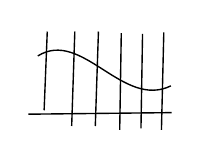
\begin{tikzpicture}[x=1cm,y=1cm,line width=.5pt]
\draw (0,0.05)--(0.04,1.05);
\draw (0.35,-0.15)--(0.39,1.05);
\draw (0.65,-0.15)--(0.69,1.05);
\draw (0.96,-0.2)--(0.98,1.03);
\draw (1.23,-0.18)--(1.25,1.02);
\draw (1.49,-0.2)--(1.52,1.04);
\draw (-0.2,0)--(1.62,0.02);
\draw (-0.08,.74)..controls (.48,1.09) and (1.00,.06)..(1.61,.36);
\end{tikzpicture}}\endgroup
}
\end{GelfandAdjacentEvidence}
\begin{GelfandAdjacentEvidence}{GELFAND-P001011}{4}

\[
\text{Тогда }\int_{\substack{\text{гориз.}\\\text{слой}}}\Omega=0.
\]
Стр. другой класс $s$

\underline{Предл.} 2
\[
\begin{aligned}
s(\mathbb R^n)&\ne0\quad n\text{ чётном}\\
&=0\quad n\text{ нечётном}
\end{aligned}
\]

\underline{\underline{Milnor}}.

$G$ --- гр. Ли, $G^\delta$ --- та же с дискр. топологией.
\[
\begin{gathered}
G^\delta\longrightarrow G\\
BG^\delta\longrightarrow BG
\end{gathered}
\]
\[
H_*\left(\qquad\begin{matrix}\mathbb Q\\\mathbb Z\\\mathbb Z_p\end{matrix}\right)\ -\ ?
\]
\Unclear{GELFAND-P001011}{milnor-coefficients}{В скобках оставлено пустое место слева от столбца $\mathbb Q,\mathbb Z,\mathbb Z_p$.}
\end{GelfandAdjacentEvidence}


$H_*(BG)$ хорошо изв. и хорошо себя ведут

$H_*(BG^\delta)$ --- ?

неизвестны и нехорошо себя ведут, неясно, полезны ли?

В алгебр. $K$-теории, в теории слоений, в 3-й пробл. Гильберта

--- всё это возникает. \qquad (равносоставленность)


\Needspace{7\baselineskip}
\begin{GelfandAdjacentEvidence}{GELFAND-P001012}{1}
\SourcePage{GELFAND-P001012}{16}
\underline{Гипотеза об изоморфизме:}
\[
(1)\qquad H_*(BG^\delta,\mathbb Z/p)\overset{\simeq}{\longrightarrow}
H_*(BG,\mathbb Z/p);\qquad \underline{\forall\ \text{простого }p.}
\]
К 3-й пробл. Гильб. это применили H. Sah, Dupont.

Когда равносоставимы? Частичн. ответ --- из когомологий классиф. пр-ва.

Вероятно (1) --- очень трудное утв.

\underline{Chern--Weyl:} $G$ компактна $\Rightarrow$
\[
\widetilde H_*(BG^\delta,\mathbb Q)\overset{0}{\longrightarrow}
\widetilde H_*(BG,\mathbb Q).
\]
(отобр. тривиально)

\underline{Sah--Wagoner}:
\Unclear{GELFAND-P001012}{upper-sah-name}{Вторая фамилия читается «Wagoner».}
\end{GelfandAdjacentEvidence}
\begin{GelfandAdjacentEvidence}{GELFAND-P001012}{2}

\[
\underset{\text{связна}}{G}\ne1
\quad\Rightarrow\quad\exists\ \text{эпиморфизм}
\]
\[
H_2(BG^\delta,\mathbb Z)\longrightarrow
\underset{\substack{\text{несчёт.}\\\text{сумма}}}{\bigsqcup}\mathbb Q\longrightarrow0
\]
В то же время:
\par $H_2(BG,\mathbb Z)$ конечно порождена.

\underline{Обсудим свид. в пользу (1).}

\tikz[baseline=(n.base)]{\node[draw,circle,inner sep=1pt](n){1};}
(1) верно в спец. случае, если алг. Ли $\mathfrak g$ разрешима.

Д-во элементарно.
\[
\bar B G\longrightarrow BG^\delta\longrightarrow BG
\]
[Под $\bar B G$ с вертикальной чертой:] по инд. док., что когом. $\bar B G$ трив.

\tikz[baseline=(n.base)]{\node[draw,circle,inner sep=1pt](n){2};}
Пусть $G$ им. конечное число компонент.

Тогда (1) --- эпим. и расщепляется.
\[
H_*(BG^\delta,\mathbb Z/p)
\underset{\underline{\mathrm{split}}}{\longrightarrow}
H_*(BG,\mathbb Z/p)\longrightarrow0
\]
\Unclear{GELFAND-P001012}{middle-arrow-cancellation}{Над стрелкой зачёркнуты короткие штрихи, возможно «эп.».}
\end{GelfandAdjacentEvidence}
\begin{GelfandAdjacentEvidence}{GELFAND-P001012}{3}


[Слева зачёркнутый знак.] (2)\quad \underline{Следствие.}
\Unclear{GELFAND-P001012}{left-margin-cancelled-number}{Перечёркнутый петлеобразный знак слева от (2) не разобран.}
\end{GelfandAdjacentEvidence}
\begin{GelfandAdjacentEvidence}{GELFAND-P001012}{4}


\SourceFigure{GELFAND-P001012}{middle-cohomology-arrow}{У средней стрелки видны оба наконечника. Под выражением скобка.\par\smallskip
\begingroup\color{black}\GelfandFitDiagram{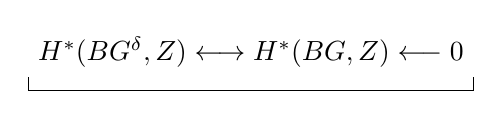
\begin{tikzpicture}
\node (seq) {$H^*(BG^\delta,\mathbb Z)\longleftrightarrow H^*(BG,\mathbb Z)\longleftarrow0$};
\draw (seq.south west) -- ++(0,-.17) -| (seq.south east);
\end{tikzpicture}}\endgroup
}
\end{GelfandAdjacentEvidence}
\begin{GelfandAdjacentEvidence}{GELFAND-P001012}{5}


Общ. --- теор. [зачёркнуто: Ду?] Bott--Heitsch.
\Unclear{GELFAND-P001012}{lower-bott-cancellation}{Под зачёркиванием перед Bott--Heitsch возможно «Ду».}
\end{GelfandAdjacentEvidence}
\begin{GelfandAdjacentEvidence}{GELFAND-P001012}{6}


\tikz[baseline=(n.base)]{\node[draw,circle,inner sep=1pt](n){3};}
(1) всегда верно [зачёркнуто: при] для $H_1$ и в интересных случаях для $H_2$:
\[
\operatorname{SL}_n\mathbb R,\quad \operatorname{SL}_n\mathbb C.
\]
\Unclear{GELFAND-P001012}{lower-sl-cancellation}{Под строкой между индексом $n$ и $\mathbb R$ густо зачёркнут знак, возможно $\mathbb Z$.}
\end{GelfandAdjacentEvidence}
\begin{GelfandAdjacentEvidence}{GELFAND-P001012}{7}


\underline{Хефлигер.}

$\operatorname{PSL}_2(\mathbb Z)$ на $\operatorname{Im}z>0$.

(др.-лин. преобр. [зачёркнуто: ко?] с целыми коэфф.)
\Unclear{GELFAND-P001012}{lower-fractional-cancellation}{В зачёркнутом фрагменте возможны начальные буквы «ко».}
\end{GelfandAdjacentEvidence}
\begin{GelfandAdjacentEvidence}{GELFAND-P001012}{8}


\SourceFigure{GELFAND-P001012}{circle-boundary}{Окружность и подпись к её границе.\par\smallskip
\begingroup\color{black}\GelfandFitDiagram{\begin{tikzpicture}[x=1cm,y=1cm]
\draw (0,0) ellipse (.57 and .48);
\node[anchor=west] at (.88,.08) {прямая ---};
\node[anchor=west] at (.88,-.28) {--- окр.};
\node[anchor=west] at (-.23,-.80) {$S^1$ --- гран.};
\end{tikzpicture}}\endgroup
}
\end{GelfandAdjacentEvidence}
\begin{GelfandAdjacentEvidence}{GELFAND-P001012}{9}


$\gamma_1,\gamma_2$ --- \underline{образующие}.
\[
\gamma_1:z\longmapsto z+1;\qquad
\gamma_2:z\longmapsto-\frac{1}{z}.
\]
$\forall f\in C^\infty(S^1),\quad\exists?\,C^\infty$-ф-и $f_1,f_2\in C^\infty(S^1)$
\Unclear{GELFAND-P001012}{exists-question}{После $\exists$ стоит знак вопроса с отдельной точкой.}
\end{GelfandAdjacentEvidence}



\Needspace{7\baselineskip}
\SourcePage{GELFAND-P001013}{unlabelled}
\[
(1)\qquad f(x)=f_1(x)-f_1(\gamma_1(x))+f_2(x)-f_2(\gamma_2(x)).
\]
Это связано со слоениями на рим. мн-зии, слои к-рых явл. \underline{мин} пов.

\underline{Неизвестно}!

Приблизительно верно: аппроксимировать можно ( в $C^\infty$-топ. ) --- это легко.


\Needspace{7\baselineskip}
\begin{GelfandAdjacentEvidence}{GELFAND-P001014}{1}
\SourcePage{GELFAND-P001014}{unlabelled}
15/\underline{III}-82.\qquad \underline{Сем. Гельфанда.}

\underline{Темы} (курсовых работ, дипл. работ и т. д.)

\underline{Кириллов}:

\SourceFigure{GELFAND-P001014}{weight-branches}{Верхняя и нижняя черты ведут к двум отдельным пунктам.\par\smallskip
\begingroup\color{black}\GelfandFitDiagram{\begin{tikzpicture}[font=\small,x=.8cm,y=.8cm]
\node[anchor=east] at (0,0) {1. \underline{Кратность веса}};
\draw (.15,.11)--(.80,.47);
\draw (.23,-.21)--(.85,-.21);
\node[anchor=west,align=left] at (.95,.78) {комп. группы Ли $\to$\\\quad Гийемин, Стернберг\\\quad в принципе получили ответ.};
\node[anchor=west] at (.95,-.30) {гиперболич. алгебры};
\end{tikzpicture}}\endgroup
}
\end{GelfandAdjacentEvidence}
\begin{GelfandAdjacentEvidence}{GELFAND-P001014}{2}

\SourceFigure{GELFAND-P001014}{weight-response}{Стрелка после «комп. группы Ли» ведёт к Гийемину и Стернбергу.}
\end{GelfandAdjacentEvidence}


\underline{Лит-ра}: \underline{Мак-дональд} (статья)

\underline{Пример} \underline{зад.} в \underline{2}: рассм. контрагредиентная алгебра Ли с гиперболич. матрицей Картана (имеющей отриц. соб. значение).

Рассм. действие $SU(3)$ на её алгебре Ли:
\[
X=\begin{pmatrix}
i\varphi_1&a&c\\
-\bar a&i\varphi_2&b\\
-\bar c&-\bar b&i\varphi_3
\end{pmatrix},\qquad
\varphi_1+\varphi_2+\varphi_3=0
\]
\[
g\in SU(3)\Rightarrow g:X\to gXg^*.
\]


\Needspace{7\baselineskip}
\begin{GelfandAdjacentEvidence}{GELFAND-P001015}{1}
\SourcePage{GELFAND-P001015}{unlabelled}
Рассм. орбиту $\Omega$. [отдельный штрих] Она имеет вид:
\Unclear{GELFAND-P001015}{orbit-punctuation}{После точки виден отдельный наклонный штрих. Чтение как $1$ или часть восклицательного знака не установлено.}
\end{GelfandAdjacentEvidence}
\begin{GelfandAdjacentEvidence}{GELFAND-P001015}{2}

\[
\begin{cases}
\operatorname{tr}\,\text{[зачёркнутый знак]}\,X^2=c_2,\\
\operatorname{tr}X^3=c_3
\end{cases}
\qquad (\text{и, кстати, }\operatorname{tr}X=0)
\]
\Unclear{GELFAND-P001015}{trace-cancellation}{Между $\operatorname{tr}$ и $X^2$ знак густо зачёркнут.}
\end{GelfandAdjacentEvidence}
\begin{GelfandAdjacentEvidence}{GELFAND-P001015}{3}

(по этим следам восстан. корни, а $\forall$ матр. привод. к диаг. виду)

Обозначим её: $\Omega_{c_2,c_3}$.

Орбита --- размерности 6 (общ. полож.)

Спроектир. на плоскость (2-мерн.) $(\varphi_1,\varphi_2,\varphi_3)$,
$\varphi_1+\varphi_2+\varphi_3=0$.

\SourceFigure{GELFAND-P001015}{diagonal-axes}{Три оси с подписями $\varphi_1,\varphi_2,\varphi_3$ и тремя углами $120^\circ$.\par\smallskip
\begingroup\color{black}\GelfandFitDiagram{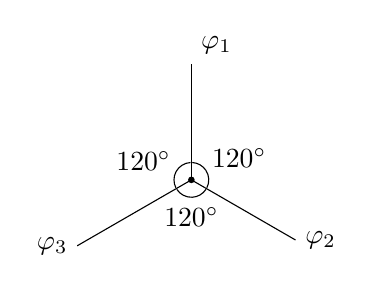
\begin{tikzpicture}[x=.92cm,y=.92cm]
\draw (0,0)--(0,1.6) node[above right] {$\varphi_1$};
\draw (0,0)--(-30:1.66) node[right] {$\varphi_2$};
\draw (0,0)--(210:1.82) node[left] {$\varphi_3$};
\fill (0,0) circle[radius=1.2pt];
\draw (93:.24) arc (93:207:.24);
\draw (213:.24) arc (213:327:.24);
\draw (333:.24) arc (333:447:.24);
\node at (-.66,.26) {$120^\circ$};
\node at (.66,.30) {$120^\circ$};
\node at (0,-.51) {$120^\circ$};
\end{tikzpicture}}\endgroup
}
\end{GelfandAdjacentEvidence}
\begin{GelfandAdjacentEvidence}{GELFAND-P001015}{4}


\SourceFigure{GELFAND-P001015}{cancelled-axes}{В зачёркнутом наброске видна стрелка вверх. Исходная геометрия и подписи под штрихами не установлены.}
\end{GelfandAdjacentEvidence}
\begin{GelfandAdjacentEvidence}{GELFAND-P001015}{5}


--- проектируем на плоскость $\varphi_1+\varphi_2+\varphi_3=0$
[зачёркнуто: неразборчиво] оси координат.
\Unclear{GELFAND-P001015}{projection-cancellation}{Перед «оси координат» зачёркнута короткая запись.}
\end{GelfandAdjacentEvidence}
\begin{GelfandAdjacentEvidence}{GELFAND-P001015}{6}


--- так надо рисовать. \qquad ($p$ --- проекция)

\underline{Факты}:

а) Проекция $\Omega_{c_1,c_2}$ заполняет 6-угольник.
\Unclear{GELFAND-P001015}{orbit-indices}{В этой строке индексы $c_1,c_2$, а в обозначении выше $c_2,c_3$.}
\end{GelfandAdjacentEvidence}
\begin{GelfandAdjacentEvidence}{GELFAND-P001015}{7}


\SourceFigure{GELFAND-P001015}{orbit-hexagon}{Шестиугольник, три выходящие стрелки и три пунктирные внутренние линии.\par\smallskip
\begingroup\color{black}\GelfandFitDiagram{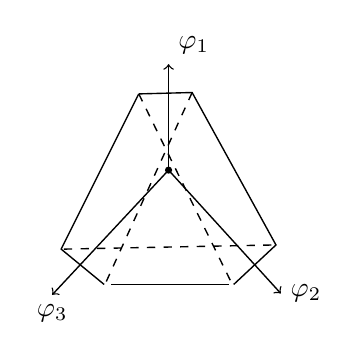
\begin{tikzpicture}[x=.88cm,y=.88cm,line width=.5pt]
\draw (-.43,1.33)--(.34,1.35)--(1.55,-.85)--(.94,-1.42);
\draw (.87,-1.42)--(-.83,-1.42);
\draw (-.93,-1.42)--(-1.55,-.91)--(-.43,1.33);
\draw[dashed] (-.43,1.33)--(.91,-1.40) (.34,1.35)--(-.90,-1.38)
(-1.51,-.91)--(1.52,-.85);
\draw[->] (0,.23)--(0,1.76) node[above right] {$\varphi_1$};
\draw[->] (0,.23)--(1.62,-1.55) node[right] {$\varphi_2$};
\draw[->] (0,.23)--(-1.68,-1.57) node[below] {$\varphi_3$};
\fill (0,.23) circle[radius=1.3pt];
\end{tikzpicture}}\endgroup
}
\end{GelfandAdjacentEvidence}
\begin{GelfandAdjacentEvidence}{GELFAND-P001015}{8}


(это мн-во диаг. элементов матриц с фиксир. набором соб. значений $\lambda_1,\lambda_2,\lambda_3$)

б) \underline{Рассм.} $p^{-1}(y_0)$, $y_0$ --- точка 6-угольника.

Это 4-мерное мн-зие. Нарушение регулярности --- на пунктирных линиях.
\Unclear{GELFAND-P001015}{fibre-dimension}{После $4$ виден горизонтальный штрих, пересечённый длинной тонкой вертикалью. Чтение «4-мерное» вероятно.}
\end{GelfandAdjacentEvidence}
\begin{GelfandAdjacentEvidence}{GELFAND-P001015}{9}


Всё это есть в раб. \underline{Березина} и \underline{Гельфанда} в Тр. ММО, 1956. \quad («Несколько замечаний к теории сферич. ф-й»)

Предст. $SU(3)$ зад. \underline{парой целых чисел} и по ним веса.

Веса --- внутри 6-угольника. Кратности:

\SourceFigure{GELFAND-P001015}{weight-contours}{Три вложенных шестиугольных контура и заштрихованный треугольник. У верхнего левого угла наложенные штрихи закрывают часть отметок.\par\smallskip
\begingroup\color{black}\GelfandFitDiagram{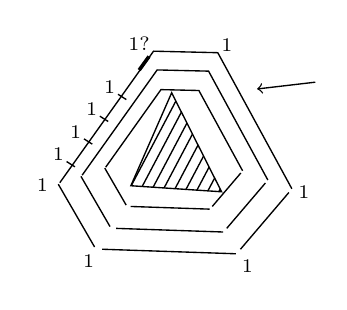
\begin{tikzpicture}[x=.96cm,y=.96cm,line width=.49pt]
\foreach \size in {1,.80,.59} {
  \begin{scope}[scale=\size]
    \draw (-1.48,-.50)--(-.24,1.24)--(.61,1.22)--(1.59,-.58);
    \draw (1.55,-.63)--(.91,-1.38);
    \draw (.85,-1.44)--(-.92,-1.38);
    \draw (-1.02,-1.35)--(-1.50,-.52);
  \end{scope}
}
\draw (0,.69)--(.66,-.62)--(-.54,-.54)--cycle;
\begin{scope}
\clip (0,.69)--(.66,-.62)--(-.54,-.54)--cycle;
\foreach \x in {-.78,-.63,-.48,-.33,-.18,-.03,.12,.27,.42,.57} {
  \draw (\x,-.72)--++(.77,1.46);
}
\end{scope}
\foreach \x/\y in {-1.71/-.54,-1.10/-1.54,1.00/-1.60,1.75/-.63,.73/1.32} {
  \node[font=\scriptsize] at (\x,\y) {$1$};
}
\foreach \x/\y in {-1.32/-.25,-1.09/.05,-.88/.35,-.64/.64} {
  \draw (\x-.07,\y+.03)--(\x+.04,\y-.04);
  \node[font=\scriptsize] at (\x-.18,\y+.12) {$1$};
}
\draw[line width=1.3pt] (-.43,.99)--(-.30,1.17);
\node[font=\scriptsize] at (-.43,1.34) {$1?$};
\draw[<-] (1.13,.74)--(1.90,.83);
\end{tikzpicture}}\endgroup
}
\end{GelfandAdjacentEvidence}
\begin{GelfandAdjacentEvidence}{GELFAND-P001015}{10}

$\leftarrow$ линии изменения кратностей

$SU(3)$ --- у Гельфанда и Березина.

Ответ \underline{Гийемина, Стернберга} --- для больших $c_2,c_3$.

[Над фамилиями, со стрелкой к ним:] препринт $\approx\underline{1981\text{~г.}}$

$X$ --- прообраз \textsuperscript{*?} точки,
$X=p^{-1}(y_0)$.
\Unclear{GELFAND-P001015}{preimage-mark}{Между «прообраз» и «точки» звёздоподобный знак, возможно зачёркнутая запись.}
\end{GelfandAdjacentEvidence}
\begin{GelfandAdjacentEvidence}{GELFAND-P001015}{11}


\[
\langle e^B\tau,X\rangle\quad\text{--- кратность!!}
\]
[Под $e^B$ черты знака равенства поставлены вертикально.]
\[
e^B=1+B+\frac{B\wedge B}{2}+\ldots
\]
$B$ --- симпл. форма на орбите.

$\tau$ --- класс Тодда мн-зия.

\underline{И. М. Г.}\qquad \underline{Осн. вопрос}: двойственность между группами и их представлениями.
\[
x^{\text{\tikz[baseline=(n.base)]{\node[draw,circle,inner sep=0.3pt] (n) {$\scriptstyle n$};}}}
=x(x-1)\ldots(x-n+1)
\]
\[
\text{\tikz[baseline=(d.base)]{\node[draw,circle,inner sep=1pt] (d) {$\frac{d}{dx}$};}}f(x)
=f(x+1)-f(x)
\]
\SourceFigure{GELFAND-P001015}{circled-operators}{Кружок вокруг $n$ и вокруг $\frac{d}{dx}$ относится к обозначениям автора.}
\end{GelfandAdjacentEvidence}



\Needspace{7\baselineskip}
\begin{GelfandAdjacentEvidence}{GELFAND-P001016}{1}
\SourcePage{GELFAND-P001016}{25}
Тогда
\SourceFigure{GELFAND-P001016}{circled-falling-factorial}{%
\(\displaystyle
\text{\tikz[baseline=(d.base)]{\node[draw,circle,inner sep=1pt] (d) {$\frac{d}{dx}$};}}
x^{\text{\tikz[baseline=(n.base)]{\node[draw,circle,inner sep=.3pt] (n) {$\scriptstyle n$};}}}
=n\,x^{\text{\tikz[baseline=(m.base)]{\node[draw,ellipse,inner sep=.4pt] (m) {$\scriptstyle n-1$};}}}\)}
\end{GelfandAdjacentEvidence}
\begin{GelfandAdjacentEvidence}{GELFAND-P001016}{2}


\Unclear{GELFAND-P001016}{cancelled-heading}{Короткая запись обведена и зачёркнута. Чтение не установлено.}
\end{GelfandAdjacentEvidence}
\begin{GelfandAdjacentEvidence}{GELFAND-P001016}{3}


Двойств.: для предст. надо смотреть кратности весов

На орбите есть (единств.) инвар. объём.

Нормировка: объём \underline{орбиты} $=$ \underline{размерности} лин. предст., с ней ассоциир.
\SourceFigure{GELFAND-P001016}{representation-abbreviation}{лин. предст., с ней ассоциир.}
\end{GelfandAdjacentEvidence}
\begin{GelfandAdjacentEvidence}{GELFAND-P001016}{4}


Многочл. Якоби
\[
\bigl(x^k(1-x)^\ell\bigr)^{(p)}=F(k,\ell,p;x)
=\int_0^x t^k(1-t)^\ell(x-t)^{-p-1}\,dt
\]
\Unclear{GELFAND-P001016}{fractional-normalization}{Между знаком равенства и интегралом множитель не указан.}
\end{GelfandAdjacentEvidence}
\begin{GelfandAdjacentEvidence}{GELFAND-P001016}{5}


Все $k,\ell,p$ --- \underline{не целые}\qquad (гипергеом. ф-я Гаусса)

\underline{Дробная производная}:
\[
(x^n)^{(k)}=x^{n-k}\frac{n!}{(n-k)!}
\qquad\text{или}\qquad
\left(\frac{x^n}{n!}\right)^{(k)}=\frac{x^{n-k}}{(n-k)!}
\]
и заменяем $!$ на $\Gamma$.

Нет удовлетв. теории \underline{гипергеом. ф-й многих} перем. (важно для предст.)

\underline{Атья}: обобщение тем, что точки $\in$ вып. многоугольнике, на случай действия только картан. группы.

Идея: переделать всю теорию предст. на действие карт. группы.

\underline{Лит-ра}: 1) Березин, Гельфанд\quad 2) Атья\quad
3) Гийемин, Стернберг\quad 4) Хованский

\SourceFigure{GELFAND-P001016}{newton-reference}{%
о многогр. Ньютона\par
\(\swarrow\)\par
по многоугольникам ---\par
--- ф-и кратности.\par
(и Казарновский)}
\end{GelfandAdjacentEvidence}



\Needspace{7\baselineskip}
\begin{GelfandAdjacentEvidence}{GELFAND-P001017}{1}
\SourcePage{GELFAND-P001017}{46}
\underline{29/III-82 г.}\qquad\underline{Сем. Гельфанда.}

\underline{Гивенталь.}

\underline{Т.1.} $M$ --- гладкое мн-зие, $N$ --- подмн-зие.

$\omega_0,\omega_1$ --- 2 симпл. структуры на $M$
\[
\omega_0|_{TN}=\omega_1|_{TN}
\]
Тогда $\forall x\in N$, $\exists$ окр. $U$ и диффеом.
$g:U\to U$, такие что
\[
g|_N=\mathrm{id}_N,\qquad g^*\omega_1=\omega_0.
\]

\begin{center}--- $\cdot$ ---\end{center}
\underline{A. Weinstein} док. это если
$\omega_0|_{TM|_N}=\omega_1|_{TM|_N}$.
(он писал $\omega_0|_N=\omega_1|_N$)

\begin{center}--- $\cdot$ ---\end{center}
\underline{Мораль}: не сущ. внешней симпл. геометрии для подмн-зия.

\begin{center}--- $\cdot$ ---\end{center}
Есть и глобальные формулировки.

\begin{center}--- $\cdot$ ---\end{center}
\underline{Идея док-ва}: взять сем-во $g_t$, $\omega_t$
\Unclear{GELFAND-P001017}{proof-superscript}{Над $g_t$ зачёркнут знак, возможно звёздочка.}
\end{GelfandAdjacentEvidence}
\begin{GelfandAdjacentEvidence}{GELFAND-P001017}{2}


\SourceFigure{GELFAND-P001017}{proof-annotations}{%
\begin{tabular}{@{}cc@{}}
\(g_t\) & \(\omega_t\)\\
\(\vert\) & \(\diagdown\)\\
диффеом. & симпл. структ.
\end{tabular}}
\end{GelfandAdjacentEvidence}
\begin{GelfandAdjacentEvidence}{GELFAND-P001017}{3}

\[
g_t^*\omega_t=\omega_0.
\]
Дифференцируем и потом используем теорему сущ. и ед. д.у. (свод. к лин. задаче)

$N=\{*\}$ $\Rightarrow$ новое док-во теор. Дарбу.

[Вопрос: при каких условиях на 2-форму она получ. ограничением из симплектич. формы.
\Unclear{GELFAND-P001017}{restriction-cancellation}{Зачёркнуто короткое слово.}
\end{GelfandAdjacentEvidence}
\begin{GelfandAdjacentEvidence}{GELFAND-P001017}{4}

необх. условие: $d\omega=0$].

\underline{И.М.Г.} Не надо ещё написать условие замкнутости:
симпл. структура в $\forall$ кас. пр-ве.

Симпл. форма св-в не имеет.

\begin{center}--- $\cdot$ ---\end{center}
\underline{Симплектич. структура в пр-ве многочленов.}

($\Rightarrow$ лагр. мн-зия с особенностями)

\SourceFigure{GELFAND-P001017}{surface-extremals}{%
\begingroup\color{black}\GelfandFitDiagram{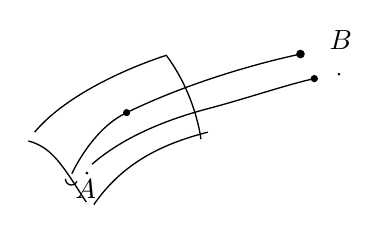
\begin{tikzpicture}[x=.80cm,y=.80cm,line width=.48pt]
\draw (0,.72) .. controls (.46,1.27) and (1.36,1.70) .. (2.09,1.94)
 .. controls (2.36,1.58) and (2.57,1.09) .. (2.64,.61);
\draw (2.75,.72) .. controls (2.05,.54) and (1.41,.25) .. (.94,-.43);
\draw (.82,-.39) .. controls (.46,.16) and (.29,.48) .. (-.10,.58);
\draw (.59,.06) .. controls (.74,.37) and (1.04,.83) .. (1.46,1.03)
 .. controls (2.18,1.38) and (3.16,1.73) .. (4.22,1.96);
\draw (.91,.21) .. controls (1.39,.63) and (2.06,.91) .. (2.74,1.09)
 .. controls (3.35,1.25) and (4.02,1.48) .. (4.44,1.57);
\draw (.49,-.02) arc[start angle=177,end angle=337,radius=.095];
\fill (.83,.07) circle[radius=.55pt];
\fill (1.46,1.03) circle[radius=1.30pt];
\draw[fill=black] (4.22,1.96) circle[radius=1.30pt];
\draw[fill=black] (4.44,1.57) circle[radius=1.05pt];
\fill (4.83,1.64) circle[radius=.52pt];
\node[below right,inner sep=.4pt] at (.62,-.01) {$A$};
\node[above right,inner sep=1pt] at (4.63,1.98) {$B$};
\end{tikzpicture}}\endgroup\par
Мелкие штрихи у $A$ не дают точно установить соединение двух линий.}
\end{GelfandAdjacentEvidence}
\begin{GelfandAdjacentEvidence}{GELFAND-P001017}{5}


$A$ --- точка на пов.

$B$ --- ---''--- вне пов. --- произвольная.

ищем экстремали (геодез. срываются)

А. \underline{Пр-во прямых в $\mathbb{R}^3$ имеет естеств. симпл. структуру!}

Б. \underline{Обобщение}: \underline{пр-во экстремалей любой вар. задачи имеет симпл. структуру}.

А. оно есть $T^*\mathbb{R}^2$ (объясн. Арнольда)

\underline{Пример}:

\SourceFigure{GELFAND-P001017}{sphere-extremals}{%
\begingroup\color{black}\GelfandFitDiagram{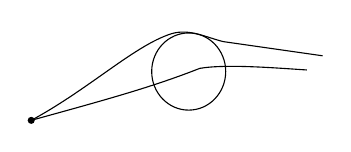
\begin{tikzpicture}[x=1cm,y=1cm]
\fill (0,0) circle (0.045);
\draw (2.0,.62) ellipse (.47 and .49);
\draw (0,0) .. controls (.74,.40) and (1.31,.95) .. (1.78,1.10)
 .. controls (2.01,1.17) and (2.23,1.05) .. (2.44,1.00) -- (3.70,.82);
\draw (0,0) .. controls (.94,.26) and (1.53,.42) .. (2.14,.66)
 .. controls (2.48,.72) and (3.17,.66) .. (3.50,.64);
\end{tikzpicture}}\endgroup}
\end{GelfandAdjacentEvidence}
\begin{GelfandAdjacentEvidence}{GELFAND-P001017}{6}


точка и сфера: возникает 2-мерное мн-зие экстремалей.

\begin{center}--- $\cdot$ ---\end{center}
Рассм. пр-во бинарных форм $\bigl\{\sum_0^{2n-1}a_i x^i y^{2n-1-i}\bigr\}$
и в нём предст. группы $SL_2(\mathbb{R})$.
\Incomplete{GELFAND-P001017}{binary-cancelled-line}{Фраза зачёркнута. Возможно, начинается «Это пр-во» или «На пр-ве». Полное чтение не установлено.}
\end{GelfandAdjacentEvidence}
\begin{GelfandAdjacentEvidence}{GELFAND-P001017}{7}

При $y=1$ --- просто многочл. степ. $2n-1$.

$w=\dfrac{x}{y}$ --- неоднор. координата.
Запишем в ней многочлен в коорд. Дарбу:
\[
\frac{q_1w^{2n-1}}{(2n-1)!}+\ldots+\frac{q_nw^n}{n!}
+\frac{p_nw^{n-1}}{(n-1)!}\mathrel{\boxed{?}}
\frac{p_{n-1}w^{n-2}}{(n-2)!}+\ldots+(-1)^{n-1}\frac{p_1w^0}{0!}
\]
\Unclear{GELFAND-P001017}{polynomial-overwritten-sign}{Знак перед членом с $p_{n-1}$ исправлен. Видны две горизонтали и нижний вертикальный штрих. Окончательное чтение не установлено.}
\end{GelfandAdjacentEvidence}



\Needspace{7\baselineskip}
\SourcePage{GELFAND-P001018}{unlabelled}
\[
\omega=\sum_{i=1}^{n}dp_i\wedge dq_i
\]
Действие $SL_2(\mathbb{R})$ сохр. форму.

$w\mapsto w+t$ \underline{гамильтонов поток}; т.к. получ. из
$\begin{pmatrix}1&t\\0&1\end{pmatrix}$

Гамильтониан:
\[
h=q_n^2/2-q_{n-1}p_n-\ldots-q_1p_2
\]
$q_1$ --- 1-й интеграл.

Рассм. редукцию $q_1=1$ и на ней пр-во хар-к.

(берём ещё $p_1=1$ --- это условно)

\underline{Вопрос И. Гольдшейда.}

Рассм. симпл. пр-во с кан. базисом $e_1,\ldots,e_n,f_1,\ldots,f_n$

Пусть $L$ --- лагр. плоскость в нём.
Верно ли, что сущ. (лагр.) плоскость $L_1$, натян. на векторы $\varphi_1,\ldots,\varphi_n$, где
$\varphi_j=\alpha_j e_j+\beta_j f_j$, такое, что
\[
\rho(L,L_1)\le 1/\sqrt{2}
\]
(годится $<1-\varepsilon$, где $\varepsilon>0$ не зависит от размерности)

Здесь $\rho(L,L_1)=\|P_L-P_{L_1}\|$, где берётся норма (операторная) в станд. евкл. метрике в базисе
$e_1,\ldots,e_n,f_1,\ldots,f_n$.

Утверждается, что $\exists\varphi_j$ такое, что $\sin(\widehat{\varphi_j,L})\le 1/\sqrt{2}$.


\Needspace{7\baselineskip}
\begin{GelfandAdjacentEvidence}{GELFAND-P001019}{1}
\SourcePage{GELFAND-P001019}{unlabelled}
\underline{\underline{5/IV-82 г.}}\qquad\underline{Сем. Гельфанда.}

\underline{\underline{Водзицки}}

$M$ --- мн-зие (возможно, с краем $\partial M$)

$D$ --- система дифф. ур-й на $M$:
\[
(1)\qquad D:C^\infty(M,E)\longrightarrow C^\infty(M,E)
\]
\underline{эллиптически опрд.} ($\sigma_D$ обратим).

\Unclear{GELFAND-P001019}{eq-two-cancel}{Перед номером (2) зачёркнут знак. Чтение не установлено.}
\end{GelfandAdjacentEvidence}

\[
(2)\qquad \operatorname{index}D=\dim\ker D-\dim\operatorname{Coker}D
=\int_M\alpha_0(x)\qquad\text{(Атья--Зингер)}
\]
[Под $\alpha_0(x)$: \underline{плотность}.]

(2) --- пример локальной формулы.

Коэфф. $\alpha_0$ выраж. через символ. Здесь естеств. появл. $\zeta$-ф-я
\[
(3)\qquad \zeta_A(s)=\sum_{\lambda\in\operatorname{Spec}A}\lambda^{-s}
\]
\[
A=D^*D,\quad DD^*.
\]
\[
z_j=\frac{n-j}{m}\quad\text{--- полюса},\qquad
n=\dim M,\quad m=\text{порядок }A.
\]
\[
z_j=0,-1,-2,\ldots\quad\text{--- \underline{полюсов нет}.}
\]
\[
\int_M\underbrace{\zeta_A(0;x)}_{\text{плотность}}=\zeta(0);
\qquad \zeta_A(0;x)\text{ явно вычисляется}
\]
\[
(4)\qquad \operatorname{index}D=\zeta_{1+D^*D}(0)-\zeta_{1+DD^*}(0)
\]


\Needspace{7\baselineskip}
\begin{GelfandAdjacentEvidence}{GELFAND-P001020}{1}
\SourcePage{GELFAND-P001020}{unlabelled}
\[
(5)\qquad
\zeta_A(0;x)=-\frac1m\int_{|\xi|=1}d\xi'
  \int_0^\infty\operatorname{tr} b^0_{-m-n}(x,\xi,\lambda)\,d\lambda
\]
\Unclear{GELFAND-P001020}{eq-five-cancel}{После знака равенства перед $-1/m$ знак или множитель зачёркнут.}
\end{GelfandAdjacentEvidence}
\begin{GelfandAdjacentEvidence}{GELFAND-P001020}{2}

\Unclear{GELFAND-P001020}{parametrix-superscript}{Над $b$ написан малый овал. Возможны $0$, $o$ или $\circ$.}
\end{GelfandAdjacentEvidence}
\begin{GelfandAdjacentEvidence}{GELFAND-P001020}{3}


[От $b^0_{-m-n}$ проведена линия к пояснению справа:]
компонента символа параметрикса $(A-\lambda)$ в нек-рой карте.

$\zeta_A(0;x)\,dx$ --- это плотность (!) --- не очевидно.

Пусть $\partial M\ne\varnothing$.
\SourceFigure{GELFAND-P001020}{upper-boundary-condition}{В рукописи стоит $\partial M\ne\varnothing$.}
\end{GelfandAdjacentEvidence}
\begin{GelfandAdjacentEvidence}{GELFAND-P001020}{4}


$D$ --- опер. сигнатуры (Дирака)

Для него:
\[
(6)\qquad \operatorname{index}D=\operatorname{sign}M
\]
\[
(7)\qquad \int_M L_k(p)=\operatorname{index}D=\int_M\alpha_0(x)
\]
\[
D:\Omega_+\longrightarrow\Omega_-
\]
$\Omega_\pm$ --- формы, чётные (неч.) отн. инволюции
$\tau=i^{np+n+1}*$ (на $p$-формах).
\[
(8)\qquad d+d^*=D|_{\Omega_+}:\Omega_+\longrightarrow\Omega_-.
\]

\underline{Пример} (И.М.Г.)
\[
(9)\qquad
\begin{pmatrix}0&\operatorname{div}\\\operatorname{grad}&\operatorname{rot}\end{pmatrix}^{2}
=\Delta\underset{\text{ед. матр.}}{I}\qquad\text{(в }R^4\text{)}
\]

\[
(10)\qquad \underline{\text{Теорема.}}\quad L_k(p)=\alpha_0(x)
\qquad\text{(Atiyah--Bott--Patodi)}
\]
\[
n=4\quad\Rightarrow\quad\alpha_0(x)=\frac13p_1
\]

\underline{Случай}
\Unclear{GELFAND-P001020}{kahler-cancel}{Перед $D$ знаки зачёркнуты.}
\end{GelfandAdjacentEvidence}
\begin{GelfandAdjacentEvidence}{GELFAND-P001020}{5}

\underline{$D=\bar\partial$} и $\overset{\text{метрика}}{M}$ ---
кэлерова
$\Rightarrow$ лок. совп. $\alpha_0(\ldots)$ и соств.
рода Тодда $T(p)$ (в общ. случае \underline{неверно}).
\Unclear{GELFAND-P001020}{todd-abbreviation}{Вероятно «соств.» перед «рода Тодда». Первые буквы тесно соединены.}
\end{GelfandAdjacentEvidence}
\begin{GelfandAdjacentEvidence}{GELFAND-P001020}{6}


Т.е. есть 2 лок. ф-лы, к-рые не совпадают.

$\partial M\ne\varnothing\Rightarrow$ тоже есть \underline{сигнатура}
(вырожд. форма на средних когом. --- нули не учит.)
\[
(11)\qquad
\underset{\substack{\text{топ.}\\\text{инвар.}}}{\operatorname{sign}M}
=\underbrace{\int_M L_k(p)}_{\text{лок. ф-ла}}
-\underbrace{\eta(\partial M)}_{\substack{\text{зависит}\\\text{от метрики}\\\text{на крае}}}
\]
(метр. в окр. края --- \underline{произведение}).

\underline{И.М.Г. Задача}: верно ли, что $\operatorname{sign}$ ---
\underline{единств. аддитивный} инвариант для мн-зий
\Unclear{GELFAND-P001020}{question-cancel}{Короткое слово перед «с» зачёркнуто.}
\end{GelfandAdjacentEvidence}
\begin{GelfandAdjacentEvidence}{GELFAND-P001020}{7}

с \underline{краем}?

\begin{center}--- $\cdot$ ---\end{center}
Перех. на дубль:
\SourceFigure{GELFAND-P001020}{double-diagram}{%
\begingroup\color{black}\GelfandFitDiagram{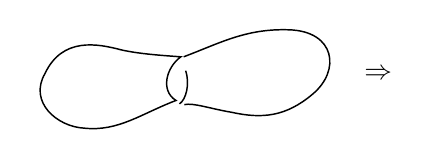
\begin{tikzpicture}[x=.88cm,y=.88cm,line width=.53pt]
\draw (0,.27) .. controls (.25,.80) and (.76,.70) .. (1.10,.61)
 .. controls (1.37,.55) and (1.69,.53) .. (1.96,.51)
 .. controls (1.75,.36) and (1.66,.02) .. (1.89,-.12)
 .. controls (1.39,-.31) and (1.06,-.57) .. (.57,-.52)
 .. controls (.17,-.50) and (-.24,-.14) .. (0,.27);
\draw (2.00,.51) .. controls (2.53,.71) and (2.90,.92) .. (3.52,.90)
 .. controls (4.19,.88) and (4.27,.31) .. (3.86,-.03)
 .. controls (3.48,-.35) and (3.14,-.39) .. (2.69,-.29)
 .. controls (2.39,-.24) and (2.14,-.15) .. (2.01,-.18);
\draw (2.03,.31) .. controls (2.09,.12) and (2.04,-.10) .. (1.94,-.17);
\node at (4.81,.25) {$\Rightarrow$};
\end{tikzpicture}}\endgroup\par
У правого штриха перетяжки сверху оставлен разрыв.}
\end{GelfandAdjacentEvidence}

видно по теор. Хирцебруха (рав. (7)),
что $\eta(\partial M)$ \underline{не зависит от заклейки}.

(12)\qquad $\eta(\partial M)$ --- нелок. инвариант!!

Локальность $\Rightarrow$ Мультиплик.
(\underline{отн.} [вставлено над строкой] перех. к накрытиям)

Есть примеры (линзовые пр-ва), когда это не так.


\Needspace{7\baselineskip}
\begin{GelfandAdjacentEvidence}{GELFAND-P001021}{1}
\SourcePage{GELFAND-P001021}{58}
(13) \underline{Теорема.} (Atiyah--Patodi--Singer)

$N=\partial M$, $D$ --- сист. 1-го порядка
\begin{equation}
D=\frac{\partial}{\partial u}+A,\qquad A\text{ --- опер. на }\partial M
\tag{14}
\end{equation}
(в окр. края)

Пусть $A$ \underline{нормальный} со спектром, не пересек. с конич. окр. $i\mathbb R$.
\Unclear{GELFAND-P001021}{spectrum-cancel}{Между «не» и «пересек.» зачёркнуто сокращение, возможно «сод.» или «соб.».}
\end{GelfandAdjacentEvidence}
\begin{GelfandAdjacentEvidence}{GELFAND-P001021}{2}


\SourceFigure{GELFAND-P001021}{margin-spectrum}{%
\begingroup\color{black}\GelfandFitDiagram{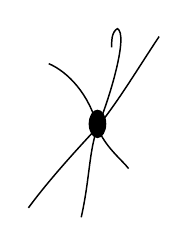
\begin{tikzpicture}[x=.86cm,y=.86cm,line width=.53pt]
\draw (-.24,-1.33) .. controls (-.11,-.74) and (-.13,-.38) .. (0,0)
 .. controls (.17,.40) and (.47,1.38) .. (.29,1.46);
\draw (.30,1.46) .. controls (.20,1.41) and (.21,1.25) .. (.21,1.18);
\draw (-1.02,-1.19) .. controls (-.69,-.74) and (-.23,-.25) .. (0,0)
 .. controls (.35,.45) and (.54,.78) .. (.91,1.34);
\draw (-.72,.94) .. controls (-.44,.82) and (-.12,.49) .. (0,0)
 .. controls (.11,-.29) and (.36,-.48) .. (.46,-.61);
\fill (0,.05) ellipse (.13 and .21);
\end{tikzpicture}}\endgroup}
\end{GelfandAdjacentEvidence}
\begin{GelfandAdjacentEvidence}{GELFAND-P001021}{3}


Тогда $\exists$ эллипт. краев. условия для $D$.

$P_A$ --- проектор на соб. знач. $A$ с $\operatorname{Re}A\geq 0$.
\SourceFigure{GELFAND-P001021}{projection-real-part}{В условии написано $\operatorname{Re}A\geq 0$.}
\end{GelfandAdjacentEvidence}
\begin{GelfandAdjacentEvidence}{GELFAND-P001021}{4}


\begin{equation}
\left\{
\begin{aligned}
Df\\
P_A(f|_A)=0
\end{aligned}
\right\}
\quad\text{--- }\underline{\text{нелок. краев. задача}}
\tag{15}
\end{equation}
\SourceFigure{GELFAND-P001021}{boundary-restriction}{Индекс ограничения в (15) написан как $A$.}
\end{GelfandAdjacentEvidence}
\begin{GelfandAdjacentEvidence}{GELFAND-P001021}{5}


лок. зад. сущ. не всегда.

Однако: всегда сущ. нелок. задача!!
\Unclear{GELFAND-P001021}{nonlocal-cancel}{После «нелок.» зачёркнут знак.}
\end{GelfandAdjacentEvidence}
\begin{GelfandAdjacentEvidence}{GELFAND-P001021}{6}


Тогда:
\begin{equation}
\operatorname{index}D=\int\alpha_0(x)-\frac{h_0+\eta(A)}{2},
\tag{16}
\end{equation}
где

$h_0=\dim$ (пр-ва чисто мнимых соб. чисел).
\Unclear{GELFAND-P001021}{kernel-cancel}{После $\dim$ зачёркнута запись, возможно $\operatorname{Ker}A$ или $\operatorname{Ker}A_0$.}
\end{GelfandAdjacentEvidence}
\begin{GelfandAdjacentEvidence}{GELFAND-P001021}{7}

\begin{equation}
\eta(A)\equiv\eta(0,A),\qquad
\eta(s,A)=\sum_{\lambda\in\operatorname{Spec}A}
\operatorname{sign}\operatorname{Re}\lambda\,
|\operatorname{Re}\lambda|^{-s}
\tag{17}
\end{equation}

\underline{Суть}: обобщение $L$-ф-и.

У A.-P.-S. \underline{$A$ --- самосопр. оператор}
\Unclear{GELFAND-P001021}{attribution-cancel}{Перед A.-P.-S. зачёркнута запись, возможно «Водз.» или «Водз».}
\end{GelfandAdjacentEvidence}
\begin{GelfandAdjacentEvidence}{GELFAND-P001021}{8}


\underline{Теорема.} $A$ --- элл. опер.
\[
\int_{N\times I}L_k(p)=\eta_{p_1}-\eta_{p_2}
\]
\Unclear{GELFAND-P001021}{cylinder-formula-symbol}{В $L_k(p)$ и в индексах $\eta$ рукописные буквы похожи на $p$. Для индексов возможно чтение $\rho$.}
\end{GelfandAdjacentEvidence}
\begin{GelfandAdjacentEvidence}{GELFAND-P001021}{9}


\SourceFigure{GELFAND-P001021}{cylinder-diagram}{%
\begingroup\color{black}\GelfandFitDiagram{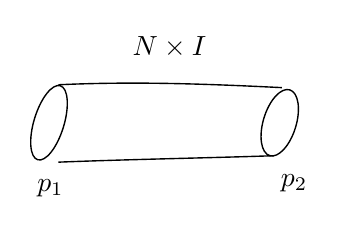
\begin{tikzpicture}[x=.91cm,y=.91cm,line width=.5pt]
\draw[rotate around={-17:(0,0)}] (0,0) ellipse (.21 and .54);
\draw[rotate around={-17:(3.22,0)}] (3.22,0) ellipse (.23 and .48);
\draw (.13,.53) .. controls (1.21,.58) and (2.24,.54) .. (3.25,.49);
\draw (.13,-.55) .. controls (1.15,-.51) and (2.28,-.49) .. (3.14,-.46);
\node at (1.68,1.05) {$N\times I$};
\node at (.02,-.91) {$p_1$};
\node at (3.42,-.84) {$p_2$};
\end{tikzpicture}}\endgroup\par
Под торцами $p_1,p_2$ или $\rho_1,\rho_2$.}
\end{GelfandAdjacentEvidence}



\Needspace{7\baselineskip}
\begin{GelfandAdjacentEvidence}{GELFAND-P001022}{1}
\SourcePage{GELFAND-P001022}{unlabelled}
\underline{12/IV — 82 г.}\qquad\underline{Сем. Гельфанда.}

\underline{Водзицки.} (\underline{Мариуш})

$X$ --- комп. мн-зие с краем.
\SourceFigure{GELFAND-P001022}{manifold-abbreviation}{В рукописи стоит сокращение «мн-зие».}
\end{GelfandAdjacentEvidence}
\begin{GelfandAdjacentEvidence}{GELFAND-P001022}{2}


(1) $D\colon C^\infty(X,E)\to C^\infty(X,F)$
эллипт. система 1-го порядка, к-рая (дифференц.)
вблизи $\partial X$ имеет вид
\[
(2)\qquad D=\frac{\partial}{\partial u}+A,\qquad
A\text{ --- оператор на краю}
\]
\[
(3)\qquad A\colon C^\infty(Y,E|_Y)\longrightarrow C^\infty(Y,F|_Y)
\]

\SourceFigure{GELFAND-P001022}{margin-spectrum}{%
\begingroup\color{black}\GelfandFitDiagram{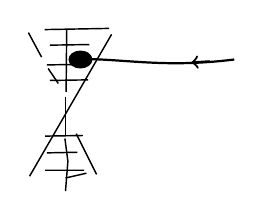
\begin{tikzpicture}[x=.76cm,y=.76cm,line width=.52pt]
\draw (-.08,-1.05) -- (-.04,-.55) -- (-.09,-.17);
\draw (-.08,-.11) -- (-.08,.53);
\draw (-.07,.61) -- (-.06,1.64);
\draw (-.68,-.80) -- (.69,1.57);
\draw (-.70,1.60) -- (-.48,1.19);
\draw (-.37,1.00) -- (-.20,.75);
\draw (.10,-.09) -- (.44,-.77);
\draw (-.43,1.65)--(.65,1.67)
      (-.34,1.39)--(.32,1.40)
      (-.39,1.06)--(.30,1.07)
      (-.34,.80)--(.30,.81)
      (-.42,-.13)--(.21,-.12)
      (-.39,-.41)--(.12,-.40)
      (-.42,-.70)--(.23,-.70)
      (-.08,-.83)--(.27,-.75);
\fill (.17,1.15) ellipse (.20 and .15);
\draw[<- ,thick] (.18,1.16) .. controls (.98,1.15) and (1.61,1.01) .. (2.74,1.15);
\draw[<- ,thick] (2.02,1.10)--(2.33,1.12);
\end{tikzpicture}}\endgroup\par
[Подпись со стрелкой:] здесь лишь конечн. число соб. значений оператора $A$.\par
У острия густые штрихи, детали соединения неразборчивы.}
\end{GelfandAdjacentEvidence}
\begin{GelfandAdjacentEvidence}{GELFAND-P001022}{3}


Краевые условия:
\[
(4)\qquad P_+f|_Y=0,
\]
$P_+$ --- проектор на полож. соб. ф-и опер. $A$.
\Unclear{GELFAND-P001022}{projection-cancellation}{Между «соб.» и «ф-и» зачёркнут знак.}
\end{GelfandAdjacentEvidence}
\begin{GelfandAdjacentEvidence}{GELFAND-P001022}{4}


(5) \underline{Теорема} (Atiyah--Patody--Singer)

1974 и последователи
\Unclear{GELFAND-P001022}{theorem-year-connector}{Короткое слово после «1974» вероятнее всего «и».}
\end{GelfandAdjacentEvidence}
\begin{GelfandAdjacentEvidence}{GELFAND-P001022}{5}


пусть

1) $A$ \underline{нормальна} отн. рим. метрики \underline{на краю}
\qquad $(A^*A=AA^*)$
\[
(6)\qquad \operatorname{index}D=\int_X\alpha_0(x)\,dx
-\frac{h(A)+\eta(A)}2
\]
\[
(7)\qquad \eta(A,s)=\sum\operatorname{sign}\operatorname{Re}\lambda\cdot
|\operatorname{Re}\lambda|^{-s},\qquad \eta(A)=\eta(A,0)
\]
\Unclear{GELFAND-P001022}{eq-seven-number}{Номер у формулы с $\eta(A,s)$ исправлен. Верхняя черта и последовательность номеров указывают на (7).}
\end{GelfandAdjacentEvidence}

\[
(8)\qquad h(A)=\dim\left\{\begin{gathered}
\text{мнимые}\\\text{соб. знач. }A
\end{gathered}\right\}
\]


\Needspace{7\baselineskip}
\begin{GelfandAdjacentEvidence}{GELFAND-P001023}{1}
\SourcePage{GELFAND-P001023}{64}
\underline{Док-во.} Используем ф-лу:
\[
(9)\qquad \operatorname{index}D=
\begin{array}[t]{c}
\operatorname{Tr}e^{-tD^*D}\\
\vert\vert\vert\\
\displaystyle\sum_{\lambda\in\operatorname{Spec}D^*D}e^{-t\lambda}
\end{array}
-
\begin{array}[t]{c}
\operatorname{Tr}e^{-tDD^*}\\
\Vert\\
\displaystyle\sum_{\mu\in\operatorname{Spec}DD^*}e^{-t\mu}
\end{array}
\]

\SourceFigure{GELFAND-P001023}{upper-left-figure}{%
\begingroup\color{black}\GelfandFitDiagram{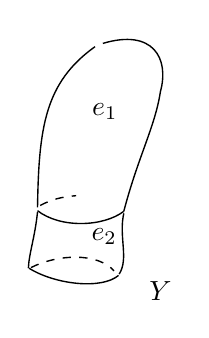
\begin{tikzpicture}[x=.83cm,y=.83cm,line width=.5pt]
\draw (0,.73) .. controls (.02,1.95) and (.11,2.64) .. (.88,3.19);
\draw (1.00,3.24) .. controls (1.77,3.47) and (2.02,3.01) .. (1.88,2.50)
 .. controls (1.80,1.97) and (1.54,1.51) .. (1.32,.67);
\draw (0,.68) .. controls (.35,.41) and (1.00,.43) .. (1.32,.67);
\draw (0,.66) .. controls (-.04,.27) and (-.13,.03) .. (-.14,-.20);
\draw (1.32,.64) .. controls (1.24,.28) and (1.40,-.05) .. (1.25,-.29);
\draw (-.13,-.20) .. controls (.27,-.45) and (.98,-.53) .. (1.24,-.31);
\draw[dashed] (-.10,-.19) .. controls (.32,.02) and (.92,.04) .. (1.17,-.24);
\draw[dashed] (.04,.76) .. controls (.23,.86) and (.37,.89) .. (.59,.91);
\node at (1.03,2.20) {$e_1$};
\node at (1.02,.29) {$e_2$};
\node at (1.88,-.55) {$Y$};
\end{tikzpicture}}\endgroup\par
Справа внизу читается $Y$. Задние дуги прерывисты.}
\end{GelfandAdjacentEvidence}
\begin{GelfandAdjacentEvidence}{GELFAND-P001023}{2}


\begin{center}--- $\cdot$ ---\end{center}

$A$ --- самосопр. эллипт. опер.
\Unclear{GELFAND-P001023}{operator-cancellation}{Перед «эллипт.» зачёркнуто слово.}
\end{GelfandAdjacentEvidence}
\begin{GelfandAdjacentEvidence}{GELFAND-P001023}{3}


\[
(10)\qquad \sum_{\lambda>0}\lambda^{-s}=\zeta_+(s),\qquad
\zeta_+(A)\text{ --- значение при }s=0.
\]

(11) $\zeta_+(A)<\infty$, но локально имеется \underline{вычет}!!
(нелокальный ф-л)

\[
(12)\qquad \zeta_+(s)=\operatorname{Tr}(P_+A^{-s})
=\int_X\operatorname{Tr}(P_+A^{-s})(x,x)
\]
[Справа: (до взятия следа были особ. при $s=i$).]
\Unclear{GELFAND-P001023}{equation-12-margin}{Знак после $s=$ похож на $i$. Над ним слабый отдельный штрих. Чтение не установлено.}
\end{GelfandAdjacentEvidence}
\begin{GelfandAdjacentEvidence}{GELFAND-P001023}{4}


Локальное слаг. имеет вычет, и $\displaystyle\int_X$ этого вычета $=0$.
\Unclear{GELFAND-P001023}{local-abbreviation}{Сокращение после «Локальное» вероятнее всего «слаг.». Конечные штрихи слабы.}
\end{GelfandAdjacentEvidence}
\begin{GelfandAdjacentEvidence}{GELFAND-P001023}{5}


\[
(13)\qquad
\left\{
\begin{aligned}
\zeta(A)&=\zeta_+(A)+\zeta_-(A)\\
\eta(A)&=\zeta_+(A)-\zeta_-(A)
\end{aligned}
\right.
\]

\underline{И. М. Г.}: в раб. Габриэлов, Гельфанд, Фукс есть алгебр. причины нелокальности.

\underline{Самая замеч. задача не сделана}: это делается для вычисл. знач. на границе форм
\underline{Понтрягина}, но \underline{для общих} классов ничего нет.
\SourceFigure{GELFAND-P001023}{pontryagin-abbreviation}{В рукописи «знач.» перед «на границе».}
\end{GelfandAdjacentEvidence}
\begin{GelfandAdjacentEvidence}{GELFAND-P001023}{6}


\[
\begin{array}{l|l|l}
\underline{\text{Stredder}}&\text{J. Diff. Geometry}&\text{о естеств. дифф. операторах.}\\
\underline{\text{Epstein}}&\underline{10}\ (1975),\ 645&\\
\text{(2 раб.)}&&
\end{array}
\]

\begin{center}--- $\cdot$ ---\end{center}

\underline{Вопрос И. М. Г.}: зачем самосопряженность $A$?

Пусть дана область и на ней опер. $A$.

\SourceFigure{GELFAND-P001023}{boundary-region}{%
\begingroup\color{black}\GelfandFitDiagram{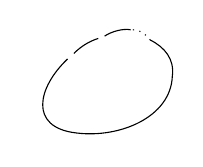
\begin{tikzpicture}[x=1cm,y=1cm]
\draw (1.42,1.25) .. controls (1.60,1.16) and (1.73,1.01) .. (1.70,.79)
 .. controls (1.68,.27) and (1.03,0) .. (.48,.07)
 .. controls (-.13,.14) and (-.01,.65) .. (.37,1.01);
\draw (.45,1.08) .. controls (.55,1.18) and (.66,1.24) .. (.76,1.27);
\draw (.84,1.30) .. controls (.93,1.36) and (1.08,1.40) .. (1.17,1.38);
\draw[dotted] (1.20,1.38) .. controls (1.31,1.38) and (1.37,1.31) .. (1.42,1.25);
\end{tikzpicture}}\endgroup}
\end{GelfandAdjacentEvidence}
\begin{GelfandAdjacentEvidence}{GELFAND-P001023}{7}


Строится теория \underline{кобордизмов}.

\underline{Инвариант} [под ним: $\eta(A)$] $A$ строится с пом. плёнки, натян. на мн-зие.
\SourceFigure{GELFAND-P001023}{manifold-abbreviation}{В рукописи стоит «мн-зие».}
\end{GelfandAdjacentEvidence}


\begin{center}--- $\cdot$ ---\end{center}

Но; в случае отсутствия заклейки не доказано!!

\begin{center}--- $\cdot$ ---\end{center}

\[
(14)\qquad \alpha_0(x)=\zeta(D^*D+\varepsilon,x)-\zeta(DD^*+\varepsilon,x)
\]


\Needspace{7\baselineskip}
\begin{GelfandAdjacentEvidence}{GELFAND-P001024}{1}
\SourcePage{GELFAND-P001024}{unlabelled}
Ф-ла для $\zeta(A,x)$
\begin{equation*}
\frac{1}{m}\int_{|\xi|=1}d\xi'\int_0^\infty
b^\circ_{-m-n}(x,\xi,\lambda)\,d\lambda
\tag{15}
\end{equation*}
\Unclear{GELFAND-P001024}{formula15-superscript}{У $b$ в (15) виден малый прерывистый овал, переданный кружком.}
\end{GelfandAdjacentEvidence}
\begin{GelfandAdjacentEvidence}{GELFAND-P001024}{2}


\SourceFigure{GELFAND-P001024}{seeley-sign-annotation}{%
\begin{tabular}{@{}l@{}c@{}}
\multicolumn{2}{@{}l@{}}{\(\uparrow\)}\\
у Сили неверный знак & \(\Vert\)
\end{tabular}}
\end{GelfandAdjacentEvidence}
\begin{GelfandAdjacentEvidence}{GELFAND-P001024}{3}


\SourceFigure{GELFAND-P001024}{angle-ray}{%
\begingroup\color{black}\GelfandFitDiagram{\begin{tikzpicture}[x=.86cm,y=.86cm]
\draw[->] (0,-.65)--(0,2.15);
\draw[->] (0,0)--(4.25,0);
\draw (0,0)--(2.05,2.15);
\draw (.65,0) arc (0:46:.65);
\node at (.88,.34) {$\theta$};
\end{tikzpicture}}\endgroup}
\end{GelfandAdjacentEvidence}
\begin{GelfandAdjacentEvidence}{GELFAND-P001024}{4}

\[
\zeta_\theta(s)=\sum\lambda^{-s}
\]
(с разрезом по лучу, идущему под углом $\theta$)

\Unclear{GELFAND-P001024}{formula16-cancellation}{Перед (16) зачёркнуто $\zeta_\theta(s)=$, вероятное чтение.}
\end{GelfandAdjacentEvidence}
\begin{GelfandAdjacentEvidence}{GELFAND-P001024}{5}

\begin{equation*}
\zeta_\theta^A(0,x)=-\frac{e^{i\theta}}{m}\int_{|\xi|=1}d\xi'
\int_0^\infty b^\circ_{-m-n}(x,\xi,e^{i\theta}\lambda)\,d\lambda
\tag{16}
\end{equation*}
(это прав. формула)
\Unclear{GELFAND-P001024}{formula16-first-argument}{Первый аргумент в (16) переписан. Возможны $0$ и $\theta$.}
\end{GelfandAdjacentEvidence}
\begin{GelfandAdjacentEvidence}{GELFAND-P001024}{6}

\Unclear{GELFAND-P001024}{formula16-superscript}{У $b$ в (16) надстрочный овал передан кружком.}
\end{GelfandAdjacentEvidence}
\begin{GelfandAdjacentEvidence}{GELFAND-P001024}{7}


\underline{И. М. Г.} \underline{Замеч. опер. в $\mathbb R^3$} (эллиптический):
\begin{equation*}
\mathcal A\varphi=
\begin{pmatrix}0&\operatorname{div}\\\operatorname{grad}&\operatorname{rot}\end{pmatrix}
\begin{pmatrix}\varphi_0\\\vec\varphi\end{pmatrix}
=(\operatorname{div}\vec\varphi,\operatorname{grad}\varphi_0+\operatorname{rot}\vec\varphi)
\tag{17}
\end{equation*}
\[
\mathcal A^2=\begin{pmatrix}\Delta&0\\0&\Delta\end{pmatrix}.
\]
\SourceFigure{GELFAND-P001024}{operator17-square}{В обеих диагональных позициях стоит $\Delta$.}
\end{GelfandAdjacentEvidence}
\begin{GelfandAdjacentEvidence}{GELFAND-P001024}{8}


\begin{center}--- $\cdot$ ---\end{center}

$A$ --- элл. опер. на замкн. мн-зии, спектр $A$ не заполняет сектора ок. луча (луч. $\min$ роста)
\Unclear{GELFAND-P001024}{spectrum-word}{Вероятнее всего «заполняет». Не исключено чтение «зацепляет».}
\end{GelfandAdjacentEvidence}
\begin{GelfandAdjacentEvidence}{GELFAND-P001024}{9}


\[
\underbrace{\zeta_{\theta,A}(s)=\sum\lambda_\theta^{-s}}_{\vphantom{\lambda}}
\qquad \text{\underline{по лучу определяем}.}
\]
\SourceFigure{GELFAND-P001024}{comparison-rays}{%
\begingroup\color{black}\GelfandFitDiagram{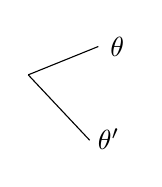
\begin{tikzpicture}[x=1cm,y=1cm]
\draw (0,.45)--(.89,.81);
\draw (0,.45)--(.78,-.38);
\node[right] at (.92,.81) {$\theta$};
\node[right] at (.76,-.37) {$\theta'$};
\end{tikzpicture}}\endgroup}
\end{GelfandAdjacentEvidence}
\begin{GelfandAdjacentEvidence}{GELFAND-P001024}{10}


Пусть $\theta'$ --- другой луч $\min$ роста.
\[
\zeta_{\theta',A}(s)=\sum\lambda_{\theta'}^{-s}
\]
$\Rightarrow$ спектр в 2-х секторах

\SourceFigure{GELFAND-P001024}{spectral-sectors-diagram}{%
\begingroup\color{black}\GelfandFitDiagram{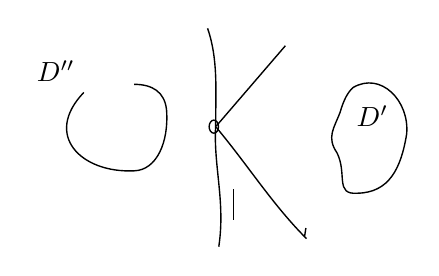
\begin{tikzpicture}[x=.79cm,y=.79cm,line width=.5pt]
\draw (-.02,1.66)..controls (.15,1.17) and (.11,.66)..(.11,.11)
..controls (.07,-.55) and (.27,-1.12)..(.16,-1.85);
\draw (.12,.09)--(1.23,1.38);
\draw (.11,.08)..controls (.63,-.54) and (1.02,-1.17)..(1.57,-1.72);
\draw (1.54,-1.68)--(1.56,-1.55);
\draw (.40,-.93)--(.40,-1.42);
\draw (.08,.08) ellipse (.075 and .105);
\draw (-2.01,.63)..controls (-2.67,-.06) and (-2.05,-.67)..(-1.20,-.63)
..controls (-.84,-.62) and (-.64,-.17)..(-.68,.35)
..controls (-.71,.64) and (-.91,.76)..(-1.20,.76);
\draw (2.32,.71)..controls (2.77,.97) and (3.23,.49)..(3.18,-.04)
..controls (3.09,-.59) and (2.90,-.98)..(2.39,-.99)
..controls (2.02,-1.02) and (2.23,-.68)..(2.06,-.34)
..controls (1.89,-.09) and (2.01,.05)..(2.11,.31)
..controls (2.17,.52) and (2.24,.64)..(2.32,.71);
\node at (-2.46,.98) {$D''$};
\node at (2.63,.25) {$D'$};
\end{tikzpicture}}\endgroup\par
Слева разрыв контура. Внизу у наклонного штриха засечка, возможно часть стрелки.}
\end{GelfandAdjacentEvidence}


(18) \underline{Теорема}.
\[
\rho(s)\overset{\mathrm{def}}{=}\zeta_\theta(A,s)-\zeta_{\theta'}(A,s)
\]
Тогда

а) $\rho(s)$ мероморфна с вычетами в $z_j=\dfrac{-j+n}{m}$, $j=0,1,2,\ldots$

б) $z_j\in\mathbb Z\Rightarrow$ вычет исчезает микролокально!!

(элементарно!)


\Needspace{7\baselineskip}
\begin{GelfandAdjacentEvidence}{GELFAND-P001025}{1}
\SourcePage{GELFAND-P001025}{65}
в)
\[
\begin{array}[t]{c}z_j\\\Vert\\\ell\end{array}
\in\mathbb Z\Rightarrow
\begin{array}[t]{c}\rho(z_j)\\\Vert\\\rho(\ell)\end{array}
\text{ зад. }\underline{\text{локальными ф-иями}}
\]
(содержат. утвержд., --- верно и для п. д. о.!)

\[
\begin{aligned}
(19)\qquad
\rho(i)&\overset{\mathrm{def}}{=}\int_X\rho_\ell(x)\,dx\\
&=-\frac{2\pi i}{m}\int_X dx\int_{|\xi|=1}d\xi'
\sum_{\lambda_\nu\in D'}\operatorname{Res}
\frac{\operatorname{tr}b^\circ_{m(i-1)-n}(x,\xi,\lambda)}{\lambda^\ell}
\end{aligned}
\]
\Unclear{GELFAND-P001025}{formula19-integer-symbol}{Аргумент в $\rho(i)$ похож на $i$, подстрочный знак в $\rho_\ell(x)$ --- на $\ell$. В пункте в) использовано $\ell$.}
\end{GelfandAdjacentEvidence}
\begin{GelfandAdjacentEvidence}{GELFAND-P001025}{2}

\Unclear{GELFAND-P001025}{formula19-b-superscript}{Над $b$ виден прерывистый овал, переданный кружком.}
\end{GelfandAdjacentEvidence}
\begin{GelfandAdjacentEvidence}{GELFAND-P001025}{3}

\Unclear{GELFAND-P001025}{formula19-power-symbol}{В индексе $b$ знак похож на $i$, а в показателе $\lambda$ --- на $\ell$.}
\end{GelfandAdjacentEvidence}
\begin{GelfandAdjacentEvidence}{GELFAND-P001025}{4}


г) $\ell\in\mathbb Z_-=\{0,-1,-2,-3,-4,\ldots\}\Rightarrow\rho(\ell)=0$

(усил. версия A.-P.-S.).

\underline{Подсказки} (к г)):

Надо док. не про вычеты в $0$, а про все целые точки $>0$
\Unclear{GELFAND-P001025}{hint-word}{Слово после «про» вероятнее всего «вычеты».}
\end{GelfandAdjacentEvidence}
\begin{GelfandAdjacentEvidence}{GELFAND-P001025}{5}

\SourceFigure{GELFAND-P001025}{hint-integer-range}{В подсказке написано \(>0\).}
\end{GelfandAdjacentEvidence}
\begin{GelfandAdjacentEvidence}{GELFAND-P001025}{6}


В точке $0$ получается: надо использовать преобр. Малера (из $p$-адич. чисел):

\[
(20)\qquad
\zeta_\theta(-k,A+t)
=\underbrace{\sum_{\nu=0}^{k}\binom{k}{\nu}\zeta(\nu-k,A)t^\nu}
_{\text{\underline{\underline{полином}}:}}
+t^k\sum_{\mu=1}^{n}
\frac{(-1)^\mu\delta_\mu}{\binom{\mu+k}{k}\mu}
\]
\Unclear{GELFAND-P001025}{formula20-second-sum}{Перед второй суммой написано $t^k$. Дополнительной степени $t$ в слагаемом не видно.}
\end{GelfandAdjacentEvidence}
\begin{GelfandAdjacentEvidence}{GELFAND-P001025}{7}


$\delta_\mu$ --- вычет в точке $\mu$ для $\zeta$-ф-и оператора $A$

Это для опер. 1-го порядка.

\[
\operatorname{Ker}A\ne\{0\}\Rightarrow
\text{вместо }\zeta(0)\text{ надо написать }\zeta(0)+h_0(A)
\]
\SourceFigure{GELFAND-P001025}{kernel-bracket}{%
\begingroup\color{black}\GelfandFitDiagram{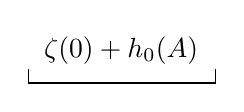
\begin{tikzpicture}[x=1cm,y=1cm]
\node at (1.18,.41) {$\zeta(0)+h_0(A)$};
\draw (0,.18)--(0,0)--(2.38,0)--(2.38,.18);
\end{tikzpicture}}\endgroup}
\end{GelfandAdjacentEvidence}
\begin{GelfandAdjacentEvidence}{GELFAND-P001025}{8}

($h_0(A)=\dim\operatorname{Ker}A$).

\Unclear{GELFAND-P001025}{mahler-cancellation}{Перед «1-я сумма» зачёркнута запись, возможно «Теор.».}
\end{GelfandAdjacentEvidence}

1-я сумма в (20) --- \underline{пр. Малера.}

Автоморфная ф-я отн. преобр. Малера продолж. в $p$-адич. область.


\clearpage
\pdfbookmark[0]{Глава 22}{gelfand-archive-chapter-22}
\section*{Глава 22}
\Needspace{7\baselineskip}
